\documentclass[11pt,a4paper,oneside]{report}
\usepackage[T1]{fontenc}
\usepackage[utf8]{inputenc}
\usepackage[italian]{babel}
\usepackage[margin=2.5cm]{geometry}
\usepackage{microtype}
\usepackage{amsmath,amssymb}
\usepackage{graphicx}
\usepackage[section]{placeins}
\usepackage{flafter}
\usepackage{caption}
\captionsetup{font=small,labelfont=bf,skip=7pt}
\captionsetup[table]{position=top}
\usepackage{booktabs,tabularx,longtable}
\usepackage{csquotes}
\usepackage{xcolor}
\usepackage{tikz}
\usetikzlibrary{arrows.meta,calc,positioning,babel,decorations.pathmorphing}
\definecolor{schemaInchiostro}{HTML}{1E1E1E}
\definecolor{schemaBlu}{HTML}{1971C2}
\definecolor{schemaVerde}{HTML}{2B8A3E}
\definecolor{schemaOcra}{HTML}{E67700}
\definecolor{schemaGrigio}{HTML}{495057}
\definecolor{schemaCartaBlu}{HTML}{E7F5FF}
\definecolor{schemaCartaVerde}{HTML}{D3F9D8}
\definecolor{schemaCartaGialla}{HTML}{FFF3BF}
\usepackage[type1,nosfdefault]{comicneue}
\newcommand{\schemafont}{\comicneueangular}
\tikzset{
  schema tratto/.style={decorate, decoration={random steps, segment length=9pt, amplitude=0.35pt}, line cap=round, line join=round},
  schema base/.style={font=\schemafont\small, text=schemaInchiostro, line width=0.95pt, execute at begin picture={\pgfmathsetseed{2718}}, every node/.append style={execute at begin node={\hyphenpenalty=10000\relax\exhyphenpenalty=10000\relax}}},
  schema blocco/.style={schema tratto, draw=schemaInchiostro, fill=schemaCartaBlu, sharp corners, align=center, inner sep=7pt, minimum height=1cm},
  schema tesi/.style={schema blocco, draw=schemaVerde, fill=schemaCartaVerde, line width=1.05pt},
  schema esterno/.style={schema blocco, draw=schemaGrigio, fill=schemaCartaGialla!55},
  schema nota/.style={font=\schemafont\footnotesize, text=schemaGrigio, align=center},
  schema freccia/.style={-{Straight Barb[length=2.6mm,width=2.4mm]}, draw=schemaInchiostro, rounded corners=4pt, line cap=round, line join=round},
  schema legame/.style={schema freccia, dash pattern=on 5pt off 3pt, draw=schemaGrigio},
  schema separatore/.style={schema tratto, draw=schemaVerde, dash pattern=on 5pt off 4pt},
  schema titolo/.style={font=\schemafont\small\bfseries, anchor=west, text=schemaInchiostro}
}
\definecolor{schemaViola}{HTML}{6741D9}
\definecolor{schemaCartaViola}{HTML}{E5DBFF}
\tikzset{
  schema icona/.style={schema tratto, draw=schemaInchiostro, line width=0.85pt, decoration={random steps, post length=1.5pt, segment length=5pt, amplitude=0.2pt}},
  schema pannello/.style={schema tratto, draw=schemaGrigio!65, fill=white, line width=0.8pt},
  schema etichetta/.style={font=\schemafont\small, align=center, text=schemaInchiostro},
  pics/pagina/.style={code={
    \path[schema icona, fill=white] (-0.7,-1) -- (0.7,-1) -- (0.7,0.7) -- (0.4,1) -- (-0.7,1) -- cycle;
    \draw[schema icona] (0.4,1) -- (0.4,0.7) -- (0.7,0.7);
    \draw[schemaBlu, line width=2pt] (-0.48,0.7) -- (0.17,0.7);
    \foreach \riga in {0.46,0.28,0.1} {\draw[schemaGrigio!75] (-0.48,\riga) -- (0.46,\riga);}
    \path[draw=schemaVerde,fill=schemaCartaVerde] (-0.48,-0.08) rectangle (-0.02,-0.64);
    \draw[schemaVerde] (-0.45,-0.5) -- (-0.27,-0.24) -- (-0.06,-0.5);
    \draw[schemaBlu, step=0.18] (0.12,-0.65) grid (0.48,-0.11);
    \draw[schemaGrigio!75] (-0.48,-0.82) -- (0.46,-0.82);
  }},
  pics/testo/.style={code={
    \path[schema icona, fill=white] (-0.55,-0.7) rectangle (0.55,0.7);
    \draw[schemaBlu,line width=2pt] (-0.34,0.45) -- (0.3,0.45);
    \foreach \riga in {0.18,-0.04,-0.26,-0.48} {\draw[schemaGrigio] (-0.34,\riga) -- (0.34,\riga);}
  }},
  pics/immagine/.style={code={
    \path[schema icona, fill=schemaCartaVerde] (-0.7,-0.5) rectangle (0.7,0.5);
    \draw[schemaVerde,line width=1pt] (-0.58,-0.36) -- (-0.15,0.18) -- (0.1,-0.11) -- (0.33,0.09) -- (0.58,-0.36);
    \fill[schemaOcra] (0.4,0.3) circle (0.08);
  }},
  pics/tabella/.style={code={
    \path[fill=schemaCartaBlu] (-0.7,0.15) rectangle (0.7,0.5);
    \draw[schema icona] (-0.7,-0.55) rectangle (0.7,0.5);
    \foreach \colonna in {-0.24,0.23} {\draw[schemaBlu] (\colonna,-0.55) -- (\colonna,0.5);}
    \foreach \riga in {-0.2,0.15} {\draw[schemaBlu] (-0.7,\riga) -- (0.7,\riga);}
  }},
  pics/vettore/.style={code={
    \foreach \colonna/\tono in {0/15,1/50,2/85,3/30,4/65} {
      \path[draw=schemaBlu,fill=schemaBlu!\tono] (0.24*\colonna-0.6,-0.2) rectangle +(0.24,0.4);
    }
  }},
  pics/archivio/.style={code={
    \path[schema icona,fill=schemaCartaGialla] (-0.8,0.55) -- (-0.8,-0.6) arc[start angle=180,end angle=360,x radius=0.8,y radius=0.24] -- (0.8,0.55) -- cycle;
    \draw[schema icona] (0,0.55) ellipse (0.8 and 0.24);
    \draw[schema icona] (-0.8,-0.05) arc[start angle=180,end angle=360,x radius=0.8,y radius=0.24];
    \draw[schema icona] (-0.8,-0.32) arc[start angle=180,end angle=360,x radius=0.8,y radius=0.24];
  }},
  pics/modello/.style={code={
    \path[schema icona,fill=schemaCartaViola] (-0.75,-0.75) rectangle (0.75,0.75);
    \foreach \posizione in {-0.5,0,0.5} {
      \draw[schema icona] (\posizione,0.75) -- (\posizione,0.96);
      \draw[schema icona] (\posizione,-0.75) -- (\posizione,-0.96);
      \draw[schema icona] (-0.75,\posizione) -- (-0.96,\posizione);
      \draw[schema icona] (0.75,\posizione) -- (0.96,\posizione);
    }
    \foreach \origine in {-0.36,0.36} {
      \foreach \destinazione in {-0.42,0,0.42} {
        \draw[schemaViola!70,line width=0.4pt] (-0.42,\origine) -- (0,\destinazione) -- (0.42,\origine);
      }
    }
    \foreach \posizione in {-0.36,0.36} {
      \fill[schemaViola] (-0.42,\posizione) circle (0.065);
      \fill[schemaViola] (0.42,\posizione) circle (0.065);
    }
    \foreach \posizione in {-0.42,0,0.42} {\fill[schemaViola] (0,\posizione) circle (0.065);}
  }},
  pics/persona/.style={code={
    \draw[schema icona,fill=schemaCartaGialla] (-0.4,0.65) circle (0.24);
    \draw[schema icona] (-0.65,-0.1) .. controls (-0.7,0.44) and (-0.08,0.45) .. (-0.06,-0.1);
    \draw[schema icona] (-0.17,0.13) -- (0.16,-0.1);
    \path[schema icona,fill=schemaCartaBlu] (0.02,-0.02) -- (0.2,0.53) -- (0.95,0.53) -- (0.76,-0.02) -- cycle;
    \draw[schema icona] (-0.9,-0.15) -- (1.1,-0.15);
    \draw[schema icona] (-0.7,-0.15) -- (-0.7,-0.65);
    \draw[schema icona] (0.9,-0.15) -- (0.9,-0.65);
  }},
  pics/cronometro/.style={code={
    \draw[schema icona,fill=schemaCartaBlu] (0,0) circle (0.5);
    \draw[schema icona] (0,0.5) -- (0,0.72) (-0.16,0.72) -- (0.16,0.72);
    \draw[schema icona] (0,0.32) -- (0,0) -- (0.25,-0.1);
  }},
  pics/checklist/.style={code={
    \path[schema icona,fill=white] (-0.6,-0.7) rectangle (0.6,0.7);
    \foreach \riga in {-0.4,0,0.4} {
      \draw[schemaVerde] (-0.44,\riga) -- ++(0.09,-0.1) -- ++(0.17,0.2);
      \draw[schemaGrigio] (-0.02,\riga) -- (0.43,\riga);
    }
  }},
  pics/cartella/.style={code={
    \path[schema icona,fill=schemaCartaGialla] (-0.8,-0.5) -- (-0.8,0.65) -- (-0.15,0.65) -- (0.03,0.43) -- (0.8,0.43) -- (0.8,-0.5) -- cycle;
    \path[schema icona,fill=schemaCartaGialla!55] (-0.8,-0.5) -- (-0.67,0.27) -- (0.94,0.27) -- (0.8,-0.5) -- cycle;
  }},
  pics/albero/.style={code={
    \draw[schemaVerde] (0,0.62) -- (0,0.28) (-0.65,-0.08) -- (-0.65,0.28) -- (0.65,0.28) -- (0.65,-0.08);
    \draw[schemaVerde] (-0.65,-0.08) -- (-0.65,-0.43) -- (-0.2,-0.43);
    \draw[schemaVerde] (0.65,-0.08) -- (0.65,-0.43) -- (0.2,-0.43);
    \foreach \centro in {(0,0.62),(-0.65,-0.08),(0.65,-0.08),(-0.2,-0.43),(0.2,-0.43)} {
      \path[draw=schemaVerde,fill=schemaCartaVerde] \centro circle (0.11);
    }
  }}
}
\tikzset{
  schema oggetto/.style={inner sep=0pt, minimum width=2.5cm, minimum height=1.9cm},
  pics/manuale-tecnico/.style={code={
    \path[schema icona,fill=schemaCartaBlu] (-0.6,-0.8) rectangle (0.82,1.02);
    \path[schema icona,fill=white] (-0.72,-0.91) rectangle (0.7,0.91);
    \node[inner sep=0pt] at (-0.01,0) {
\includegraphics[height=1.65cm]{figure/asset/copertina-manuale-fanuc.png}};
    \draw[schemaBlu,line width=1.7pt] (-0.69,-0.86) -- (-0.69,0.86);
  }},
  pics/documento-strutturato/.style={code={
    \path[schema icona,fill=white] (-1.1,-0.9) -- (0.15,-0.9) -- (0.15,0.65) -- (-0.1,0.9) -- (-1.1,0.9) -- cycle;
    \draw[schema icona] (-0.1,0.9) -- (-0.1,0.65) -- (0.15,0.65);
    \foreach \riga in {0.48,0.24,0,-0.24,-0.48} {\draw[schemaGrigio!65] (-0.9,\riga) -- (-0.05,\riga);}
    \draw[schemaVerde,line cap=round] (0.38,0.62) -- (0.38,-0.6);
    \foreach \riga/\colore in {0.45/schemaBlu,0/schemaVerde,-0.45/schemaOcra} {
      \draw[schemaVerde] (0.38,\riga) -- (0.75,\riga);
      \path[draw=\colore,fill=\colore!15] (0.75,\riga-0.13) rectangle (1.18,\riga+0.13);
    }
    \path[fill=schemaCartaVerde,draw=schemaVerde] (0.17,0.58) rectangle (0.59,0.84);
  }},
  pics/scansione/.style={code={
    \path[schema icona,fill=white] (-0.78,-0.92) rectangle (0.78,0.92);
    \foreach \riga in {0.58,0.35,0.12,-0.11} {
      \draw[schemaGrigio!35,line width=2pt] (-0.56,\riga) -- (0.54,\riga);
    }
    \foreach \riga in {0.58,0.12} {
      \path[draw=schemaBlu,densely dashed] (-0.63,\riga-0.1) rectangle (0.61,\riga+0.1);
    }
    \draw[schemaVerde,line width=1.2pt] (-1,0.62) -- (-1,1.08) -- (-0.57,1.08);
    \draw[schemaVerde,line width=1.2pt] (1,-0.62) -- (1,-1.08) -- (0.57,-1.08);
    \node[font=\ttfamily\tiny,text=schemaBlu] at (0,-0.57) {abc};
  }},
  pics/frammenti/.style={code={
    \foreach \centro/\colore in {0.63/schemaBlu,0/schemaVerde,-0.63/schemaOcra} {
      \path[schema icona,fill=\colore!12] (-1.04,\centro-0.23) rectangle (1.04,\centro+0.23);
      \draw[\colore,line width=1.5pt] (-0.84,\centro) -- (-0.58,\centro);
      \draw[schemaGrigio!70] (-0.4,\centro) -- (0.81,\centro);
    }
  }},
  pics/spazio-vettoriale/.style={code={
    \draw[schemaGrigio!55,line cap=round] (-1.05,0.88) -- (-1.05,-0.85) -- (1.1,-0.85);
    \path[fill=schemaCartaBlu] (-0.38,0.3) ellipse (0.64 and 0.48);
    \path[fill=schemaCartaVerde] (0.58,-0.38) ellipse (0.49 and 0.3);
    \foreach \ascissa/\ordinata in {-0.75/0.42,-0.4/0.6,-0.15/0.18,-0.58/0.06,0.05/0.44} {
      \fill[schemaBlu] (\ascissa,\ordinata) circle (0.065);
    }
    \foreach \ascissa/\ordinata in {0.3/-0.4,0.58/-0.22,0.78/-0.52,0.92/-0.3} {
      \fill[schemaVerde] (\ascissa,\ordinata) circle (0.065);
    }
    \draw[schemaViola,densely dashed] (-0.15,0.18) -- (0.27,0.55) -- (0.05,0.44);
    \path[draw=schemaViola,fill=schemaCartaViola] (0.27,0.55) circle (0.095);
  }},
  pics/ricerca/.style={code={
    \pic[scale=0.76] at (-0.17,0.06) {frammenti};
    \draw[draw=schemaBlu,fill=schemaCartaBlu,fill opacity=0.35,line width=1.2pt] (0.36,0.14) circle (0.52);
    \draw[schema icona,line width=2.4pt] (0.74,-0.25) -- (1.13,-0.73);
    \draw[schemaVerde,line width=1.2pt] (0.1,0.11) -- (0.28,-0.05) -- (0.63,0.32);
  }},
  pics/fascicolo/.style={code={
    \path[schema icona,fill=schemaCartaGialla] (-1.14,-0.78) -- (-1.14,0.67) -- (-0.46,0.67) -- (-0.22,0.44) -- (1.1,0.44) -- (1.1,-0.78) -- cycle;
    \foreach \ascissa/\colore in {-0.73/schemaBlu,-0.18/schemaVerde,0.37/schemaViola} {
      \path[schema icona,fill=white] (\ascissa,-0.25) rectangle +(0.61,1.2);
      \draw[\colore,line width=2.4pt] (\ascissa+0.12,0.72) -- (\ascissa+0.48,0.72);
      \foreach \riga in {0.48,0.26,0.04} {\draw[schemaGrigio!65] (\ascissa+0.12,\riga) -- (\ascissa+0.48,\riga);}
    }
    \path[schema icona,fill=schemaCartaGialla] (-1.14,-0.78) -- (-0.93,0.08) -- (1.28,0.08) -- (1.1,-0.78) -- cycle;
    \draw[schemaOcra,line width=1.4pt] (-0.3,-0.34) -- (0.46,-0.34);
  }},
  pics/dialogo/.style={code={
    \path[schema icona,fill=schemaCartaBlu] (-1.05,0.78) -- (1.05,0.78) -- (1.05,-0.38) -- (0.08,-0.38) -- (-0.47,-0.81) -- (-0.37,-0.38) -- (-1.05,-0.38) -- cycle;
    \foreach \riga in {0.48,0.2,-0.08} {\draw[schemaBlu] (-0.77,\riga) -- (0.68,\riga);}
  }},
  pics/domanda/.style={code={
    \path[schema icona,fill=schemaCartaGialla] (-0.96,0.73) -- (0.96,0.73) -- (0.96,-0.38) -- (0.05,-0.38) -- (-0.45,-0.79) -- (-0.32,-0.38) -- (-0.96,-0.38) -- cycle;
    \node[font=\schemafont\Large,text=schemaOcra] at (0,0.17) {?};
  }},
  pics/distribuzione-token/.style={code={
    \draw[schemaGrigio!55] (-1.02,-0.68) -- (1.06,-0.68);
    \foreach \ascissa/\altezza/\colore in {-0.83/0.48/schemaBlu,-0.2/1.4/schemaVerde,0.43/0.83/schemaBlu} {
      \path[schema icona,draw=\colore,fill=\colore!20] (\ascissa,-0.68) rectangle +(0.4,\altezza);
    }
    \draw[schemaVerde,line width=1.3pt] (-0.19,0.97) -- (-0.03,0.82) -- (0.29,1.16);
  }},
  pics/controllo-fonte/.style={code={
    \pic[scale=0.9] at (-0.4,0.08) {pagina};
    \pic[scale=0.9] at (0.65,-0.12) {checklist};
  }}
}
\usepackage[backend=biber,style=authoryear,maxcitenames=2,maxbibnames=99]{biblatex}
\addbibresource{bibliografia.bib}
\usepackage[
  colorlinks=true,
  linkcolor=black,
  citecolor=black,
  urlcolor=blue!60!black
]{hyperref}

\setcounter{secnumdepth}{1}
\setcounter{tocdepth}{1}
\setlength{\parindent}{1.2em}
\setlength{\parskip}{0.25\baselineskip}
\setlength{\emergencystretch}{2em}
\renewcommand{\topfraction}{0.9}
\renewcommand{\bottomfraction}{0.8}
\renewcommand{\textfraction}{0.1}
\renewcommand{\floatpagefraction}{0.75}
\setlength{\textfloatsep}{14pt plus 3pt minus 3pt}
\setlength{\intextsep}{12pt plus 3pt minus 3pt}
\AddToHook{env/table/begin}{\renewcommand{\arraystretch}{1.18}}
\renewcommand{\tabularxcolumn}[1]{>{\raggedright\arraybackslash}p{#1}}

\newif\ifnoteredazionali
\noteredazionalitrue
\newcommand{\notaredazionale}[1]{\ifnoteredazionali\par\begingroup\small\color{blue!45!black}\noindent\textbf{Nota di lavoro --- non è testo della tesi.} #1\par\endgroup\fi}

\newif\ifringraziamenti
\ringraziamentifalse

\title{Progettazione e validazione di una pipeline multimodale per l’elaborazione di manuali tecnici industriali a supporto di sistemi RAG}
\author{Nome e cognome da inserire}
\date{Anno accademico da confermare}

\begin{document}
\hypersetup{pageanchor=false}
\begin{titlepage}

\begin{center}


\includegraphics[width=6.5cm,height=4.7cm]{figure/asset/marchio-di-ateneo.png}

\vspace{10mm}

{\large\bfseries DIPARTIMENTO DI INGEGNERIA INDUSTRIALE\par}

\vspace{5mm}

{\large Corso di laurea in\par}
{\Large\bfseries INGEGNERIA GESTIONALE\par}

\vspace{10mm}

{\LARGE\bfseries Progettazione e validazione di una pipeline multimodale per l’elaborazione di manuali tecnici industriali a supporto di sistemi RAG\par}

\vspace{6mm}

{\large Tesi di laurea in Impianti Industriali\par}

\end{center}

\vspace{10mm}

\noindent\begin{minipage}[t]{0.40\textwidth}
{\large\bfseries Relatore\par}
{\large Prof. Mauro Gamberi\par}

\vspace{3mm}

{\large\bfseries Correlatore\par}
{\large Ing. Pasquale Di Nardo\par}
\end{minipage}
\hfill
\begin{minipage}[t]{0.40\textwidth}\raggedleft
{\large\bfseries Presentata da\par}
{\large Michele Mazza\par}
\end{minipage}

\vfill

\noindent\rule[0.5cm]{\textwidth}{0.6mm}

\begin{center}
{\large\bfseries Sessione Ottobre 2026\par}
{\large\bfseries Anno Accademico 2025/2026\par}
\end{center}

\end{titlepage}
\clearpage
\thispagestyle{empty}
\vspace*{0.3\textheight}
\begin{flushright}
  \itshape A Boris
\end{flushright}
\clearpage
\pagenumbering{roman}
\hypersetup{pageanchor=true}
\chapter*{Abstract}
\addcontentsline{toc}{chapter}{Abstract}

Nell'assistenza alla conduzione e manutenzione, i sistemi di \emph{Retrieval-Augmented Generation} (RAG) dipendono dalla preparazione dei manuali tecnici, le cui informazioni sono distribuite fra testo, immagini, tabelle e struttura. Nel progetto da cui nasce il lavoro, l'assistente per una macchina per elettroerosione usava un generatore \emph{text-only}: ciò che era visibile solo nelle figure, come la posizione di un comando, restava escluso. La tesi progetta e valida una pipeline multimodale locale che trasforma manuali PDF eterogenei in una rappresentazione gerarchica comune e verificabile.

La pipeline instrada ogni documento verso tre profili: PDF digitale con indice incorporato, PDF digitale con struttura da ricostruire e scansione acquisita con OCR. Un modello visuale locale descrive le immagini, le tabelle sono serializzate con regole deterministiche e provenienza e controlli sono conservati in un fascicolo di esecuzione. Il corpus comprende due manuali, uno digitale in due varianti e uno scansionato; la valutazione combina prove integrali senza captioning e due esecuzioni finali su dieci pagine.

Le prove integrali elaborano 1112 pagine su 1112 per ciascuna variante digitale, con 14.047 elementi, e 34 su 34 per il manuale scansionato. Le esecuzioni finali superano 30 controlli tecnici su 30, restando sperimentali; delle 17 richieste di captioning, otto producono descrizioni ammissibili, cinque richiedono revisione e quattro superano il limite di lunghezza.

Strategie di acquisizione diverse convergono quindi in un output comune e tracciabile. Le descrizioni aggiungono informazioni utili, ma anche errori: una caption accettata conta dieci pulsanti dove l'immagine ne mostra dodici. La conformità tecnica non garantisce la correttezza semantica; l'effetto sul RAG richiede una valutazione distinta.
\tableofcontents
\clearpage
\pagenumbering{arabic}
\chapter{Introduzione}
\label{cap:introduzione}

Questa tesi nasce nel filone di ricerca di Pasquale Di Nardo sull'impiego di assistenti basati su intelligenza artificiale nelle attività industriali. Le criticità osservate nell'uso di un assistente per una macchina per elettroerosione hanno orientato il lavoro verso la preparazione della conoscenza documentale. Il contributo sviluppato è una pipeline di ingestion integrata nell'esecuzione e modulare nella progettazione: a partire da manuali PDF eterogenei, organizza testo, immagini e tabelle in una rappresentazione gerarchica comune, sulla quale operano le successive fasi di arricchimento e verifica.

\section{Assistenza industriale e origine del lavoro}
\label{sec:assistenza-cognitiva}
\label{sec:progetto-quadro}

Le attività di conduzione e manutenzione, indicate nel seguito come \emph{operation e maintenance} (O\&M), richiedono di collegare informazioni tecniche e azioni operative. Interpretare un allarme, individuare un componente o eseguire una procedura significa consultare conoscenze distribuite tra manuali, istruzioni ed esperienza del personale. La complessità dei macchinari rende quindi rilevante non soltanto la disponibilità della documentazione, ma anche la possibilità di utilizzarla durante il lavoro \parencite{ludwig2025ontology}.

Gli assistenti digitali offrono un accesso conversazionale a questa conoscenza. Il valore del supporto dipende però dalla sua utilizzabilità nel compito: una spiegazione corretta in termini generali può non bastare a eseguire un'operazione. Per questo la valutazione degli assistenti industriali considera sia il comportamento del sistema sia l'interazione con l'utente \parencite{colabianchi2024assessment}.

In questo contesto si colloca il progetto di ricerca di Di Nardo. Nei primi colloqui di supervisione, il progetto è stato presentato a partire da un assistente basato su modelli linguistici e recupero della conoscenza dai manuali, destinato alle attività di O\&M di una macchina per elettroerosione. Il sistema è eseguito \emph{on-premise}, all'interno dell'organizzazione, senza inviare la documentazione industriale a servizi esterni. Impiega un'architettura \emph{Retrieval-Augmented Generation} (RAG), introdotta nella Sezione~\ref{sec:llm-rag}.

Nella configurazione utilizzata per l'esperimento, il generatore era Qwen3-4B, un modello \emph{text-only} della famiglia Qwen3 \parencite{qwen2025release}. Riceveva la domanda e i passaggi testuali recuperati, non le immagini del manuale. Questa configurazione costituisce il punto di partenza del lavoro, non una dimostrazione di superiorità rispetto alle alternative multimodali.

La campagna sperimentale del progetto si è evoluta da quesiti a risposta multipla all'interazione con un Digital Twin: un ambiente che riproduce l'interfaccia della macchina e permette ai partecipanti di affrontare compiti operativi in simulazione. Il confronto tra uso dell'assistente e consultazione del manuale considera tempi, accuratezza, usabilità mediante System Usability Scale (SUS), carico di lavoro percepito mediante NASA-TLX e situazioni classificate come \emph{critical failures}, rilevanti per la sicurezza o la qualità del prodotto. La Figura~\ref{fig:esperimento-dinardo} riassume le condizioni di supporto e le dimensioni osservate.

\begin{figure}[!htbp]
\centering
\begin{tikzpicture}[schema base]
\node[schema titolo] at (0,1) {Esperimento: 10 compiti, 5 coppie di difficoltà simile};
\foreach \coppia in {1,2,3,4,5} {
  \begin{scope}[shift={({0.25+3*(\coppia-1)},0)}]
    \path[schema pannello,fill=schemaCartaGialla!50] (0,-0.7) rectangle (2.65,0.4);
    \node[draw=schemaVerde,fill=schemaCartaVerde,inner sep=4pt] at (0.68,-0.12) {\coppia A};
    \node[draw=schemaBlu,fill=schemaCartaBlu,inner sep=4pt] at (1.95,-0.12) {\coppia B};
  \end{scope}
}
\node[schema pannello,fill=schemaGrigio!3,minimum width=8cm,minimum height=1.9cm,inner sep=0pt] (partecipante) at (7.5,-2.15) {};
\pic[scale=0.95] at (5.15,-2.15) {persona};
\node[schema etichetta,text width=4.5cm] at (9,-2.15) {Lo stesso partecipante\\usa entrambe le condizioni};
\draw[schema freccia] (7.5,-0.85) -- (partecipante.north);
\path[schema pannello,draw=schemaVerde,fill=schemaCartaVerde!35] (0,-3.65) rectangle (6.6,-7.4);
\path[schema pannello,draw=schemaBlu,fill=schemaCartaBlu!50] (8.4,-3.65) rectangle (15,-7.4);
\node[schema titolo] at (0.3,-4.05) {A\quad Assistente AI};
\node[schema titolo] at (8.7,-4.05) {B\quad Consultazione del manuale};
\coordinate (biforcazione) at (7.5,-3.32);
\draw[schema freccia,-] (partecipante.south) -- (biforcazione);
\draw[schema freccia,rounded corners=2pt,-{Straight Barb[length=2mm,width=2mm]}] (biforcazione) -| (3.3,-3.65);
\draw[schema freccia,rounded corners=2pt,-{Straight Barb[length=2mm,width=2mm]}] (biforcazione) -| (11.7,-3.65);
\node[draw=schemaVerde,fill=white,rounded corners=4pt,text width=3.5cm,align=center,inner sep=4pt,font=\schemafont\footnotesize] (domanda) at (2.35,-4.95) {Domanda\\dell'operatore};
\node[draw=schemaVerde,fill=white,rounded corners=4pt,text width=3.5cm,align=center,inner sep=4pt,font=\schemafont\footnotesize,below=3mm of domanda] (risposta) {Risposta dal testo\\del manuale};
\draw[schema freccia,draw=schemaVerde,-{Straight Barb[length=1.4mm,width=1.4mm]}] (domanda.south) -- (risposta.north);
\pic[scale=0.55] at (5.3,-5.45) {modello};
\node[schema etichetta] at (3.3,-6.95) {RAG locale con Qwen3-4B text-only};
\node at (9.9,-5.55) {
\includegraphics[height=1.95cm]{figure/asset/copertina-manuale-fanuc.png}};
\pic[scale=0.8] at (13,-5.45) {pagina};
\node[schema etichetta] at (11.7,-6.95) {Testo, figure e tabelle nel PDF};
\draw[schema freccia] (3.3,-7.4) -- (3.3,-7.95) -- (6.2,-7.95) -- (6.2,-8.5);
\draw[schema freccia] (11.7,-7.4) -- (11.7,-7.95) -- (8.8,-7.95) -- (8.8,-8.5);
\path[schema pannello,fill=schemaGrigio!5] (4.65,-13) rectangle (10.35,-8.5);
\draw[schemaGrigio] (4.65,-8.92) -- (10.35,-8.92);
\foreach \posizione/\colore in {4.95/schemaOcra,5.2/schemaVerde,5.45/schemaBlu} {\fill[\colore] (\posizione,-8.72) circle (0.05);}
\node[schema etichetta] at (7.75,-8.73) {Digital Twin nel browser};
\node[inner sep=0pt] at (7.5,-10.95) {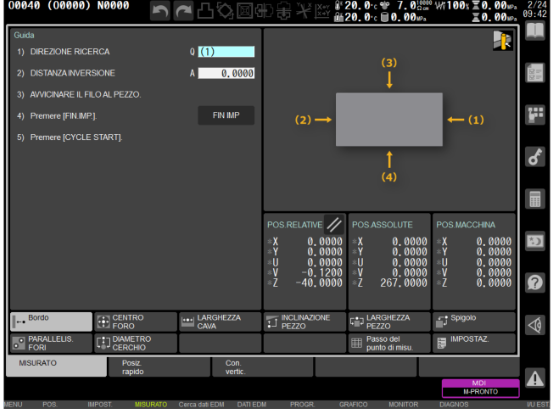
\includegraphics[width=5.15cm,height=3.85cm,keepaspectratio]{figure/asset/digital-twin.png}};
\draw[schema icona] (7.15,-13) -- (7.15,-13.25) -- (7.85,-13.25) -- (7.85,-13);
\draw[schema icona] (6.7,-13.28) -- (8.3,-13.28);
\node at (1.75,-10.4) {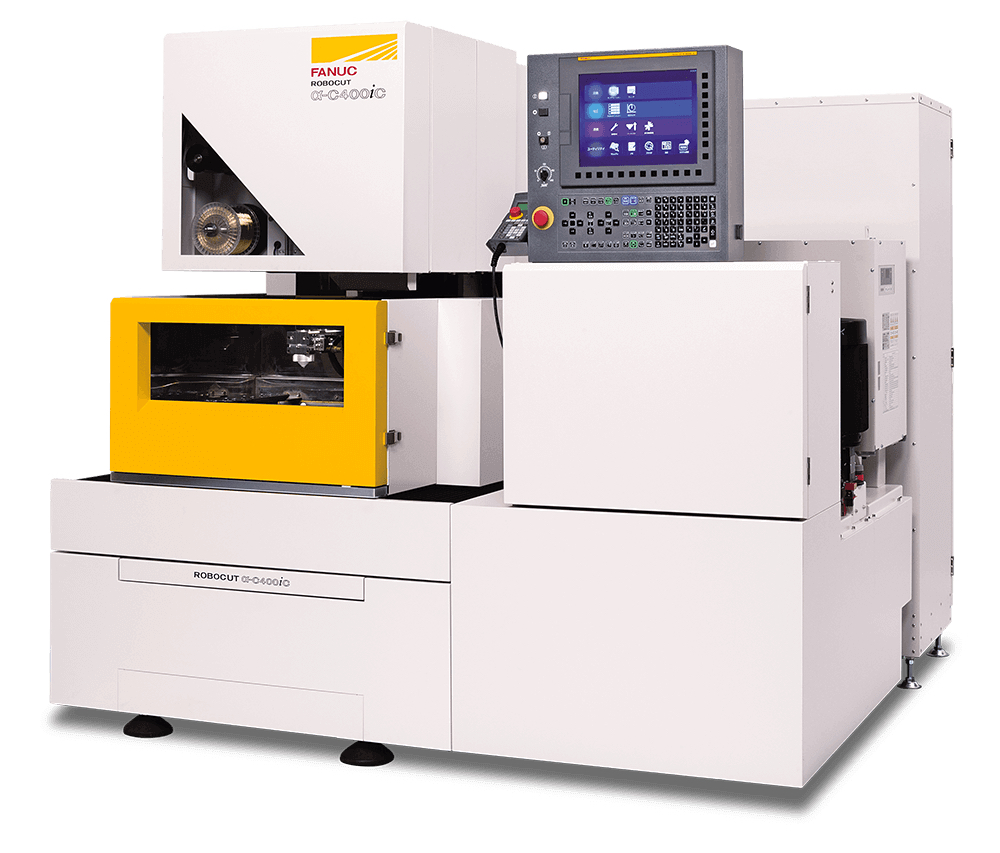
\includegraphics[width=2.85cm]{figure/asset/fanuc-robocut-c600ic-foto.jpeg}};
\node[schema nota,text width=3.35cm] at (1.75,-12.3) {Macchina di riferimento:\\la prova è in simulazione};
\draw[schema legame] (3.25,-10.4) -- (4.6,-10.4);
\node[inner sep=0pt] (operatore) at (13.15,-10.4) {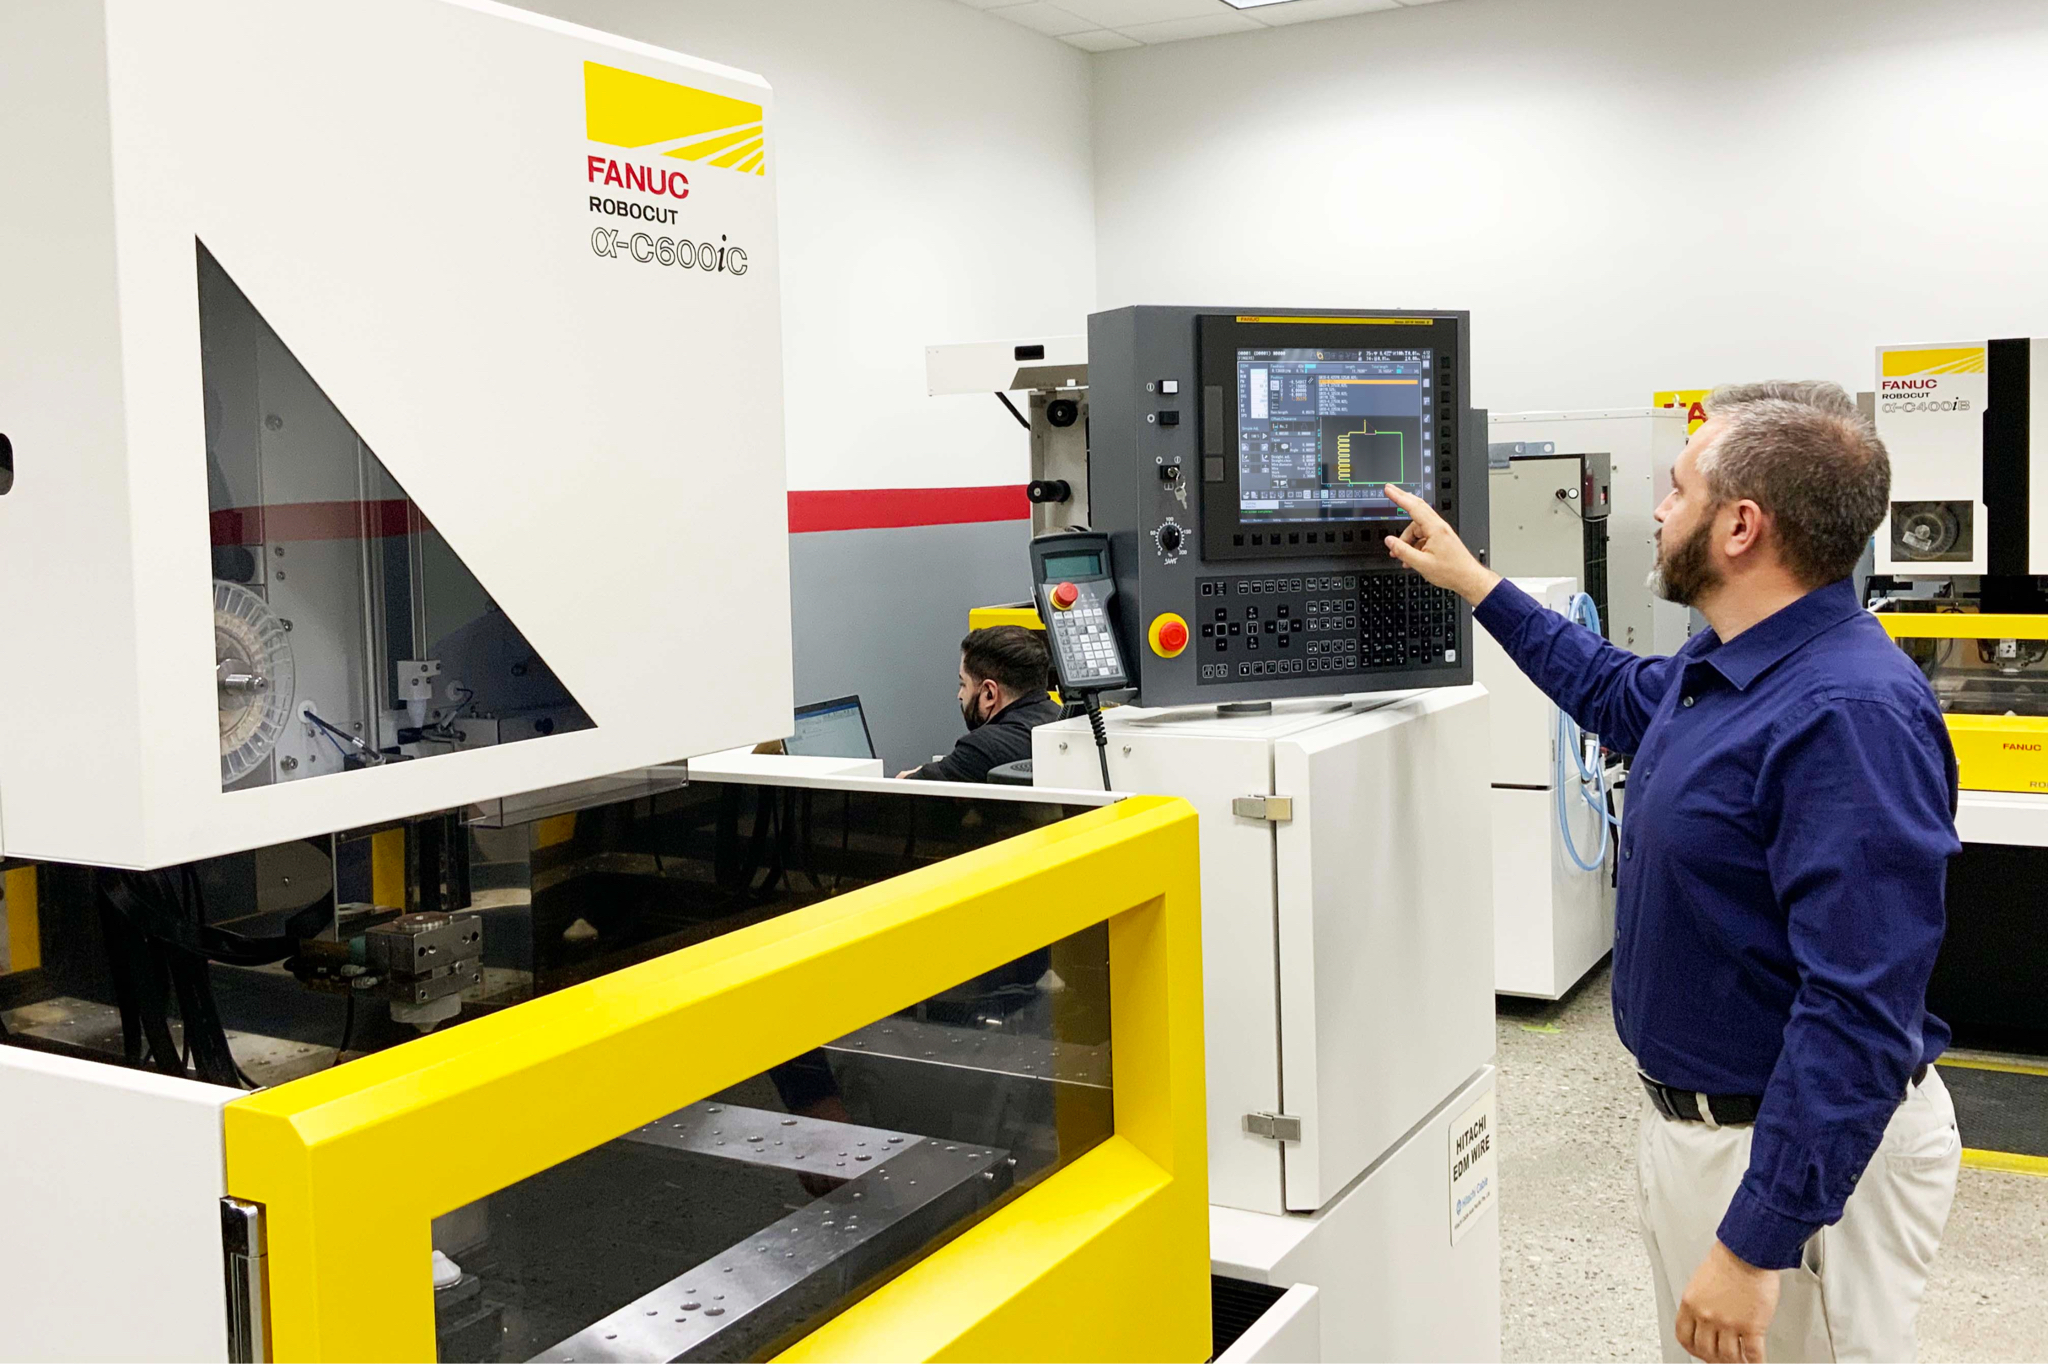
\includegraphics[width=3.6cm,height=3.85cm,keepaspectratio]{figure/asset/touch-panel-interazione-operatore.jpeg}};
\node[schema nota,text width=3.6cm,below=2mm of operatore] {L'operatore\\usa il supporto\\per individuare\\i comandi\\e svolgere il compito.};
\node[schema titolo] at (0,-14.05) {Dimensioni osservate, non risultati};
\draw[schema freccia] (7.5,-13.35) -- (7.5,-14.3);
\pic[scale=0.6] at (1.8,-15.15) {cronometro};
\pic[scale=0.6] at (5.4,-15.15) {checklist};
\path[draw=schemaOcra,fill=schemaCartaGialla,line width=1pt] (8.5,-15.5) -- (9,-14.6) -- (9.5,-15.5) -- cycle;
\node at (9,-15.24) {!};
\pic[scale=0.6] at (12.8,-15.15) {testo};
\node[schema etichetta] at (1.8,-16.1) {Tempi};
\node[schema etichetta] at (5.4,-16.1) {Accuratezza};
\node[schema etichetta] at (9,-16.1) {Critical failures};
\node[schema etichetta] at (12.8,-16.1) {SUS e NASA-TLX};
\end{tikzpicture}
\caption[Esperimento di Di Nardo: compiti, supporti e interfaccia]{Ricostruzione del progetto di Pasquale Di Nardo a partire dallo schema sperimentale fornito dall'autore della tesi. La schermata del Digital Twin è ritagliata dalla stessa figura; macchina, copertina e immagine di interazione con il touch panel provengono dai materiali allegati. Le vignette di dialogo sono schematiche, non risposte registrate. A e B indicano condizioni dello stesso partecipante, non gruppi distinti né un ordine di esecuzione. Questa sperimentazione non è la validazione finale della pipeline.}
\label{fig:esperimento-dinardo}
\end{figure}

La prova dell'assistente in laboratorio ha offerto un'occasione concreta per discutere il passaggio dalla spiegazione all'azione. Il sistema poteva fornire indicazioni generali senza aiutare a localizzare un tasto nell'interfaccia o a identificarlo rispetto ai comandi vicini. Nel dialogo con il supervisore, questa distanza è stata riassunta nell'immagine del modello come \enquote{gran teorico}. È emersa così una risorsa non utilizzata: le immagini del manuale, nelle quali una posizione può essere visibile senza essere descritta nel testo.

L'osservazione ha orientato la scelta di approfondire la componente tecnica anziché riprogettare l'esperimento sugli operatori, individuando un limite sul quale intervenire senza attribuire tutti gli errori all'assenza delle immagini. Il successivo confronto ha ampliato il problema: acquisire le figure non basta, se si perdono la gerarchia del manuale e i rapporti tra contenuti. La direzione multimodale ha quindi dato origine a un lavoro di ingestion e strutturazione documentale, nel quale l'enrichment è uno stadio e non l'intero sistema.

\section{LLM e sistemi RAG}
\label{sec:llm-rag}

I \emph{Large Language Models} (LLM) sono modelli linguistici addestrati su grandi quantità di dati. Nei modelli generativi autoregressivi, il testo viene prodotto progressivamente sulla base della sequenza disponibile, che può includere la richiesta dell'utente e informazioni aggiuntive. La conoscenza appresa nei parametri non coincide però con un archivio aggiornato dei documenti di un'organizzazione: per rispondere su un manuale specifico è utile fornire al modello le fonti pertinenti \parencite{lewis2020rag}. La Figura~\ref{fig:llm-autoregressivo} illustra il ciclo di generazione.

\begin{figure}[!htbp]
\centering
\begin{tikzpicture}[schema base]
\node[schema titolo] at (0,2.2) {Dal contesto al prossimo token};
\node[schema etichetta,font=\schemafont\small\bfseries] at (1.9,1.25) {1\quad Contesto};
\node[schema etichetta,font=\schemafont\small\bfseries] at (7.35,1.25) {2\quad Elaborazione};
\node[schema etichetta,font=\schemafont\small\bfseries] at (12.5,1.25) {3\quad Predizione};
\draw[schemaGrigio!20] (-0.05,0.82) -- (3.85,0.82);
\draw[schemaGrigio!20] (5.1,0.82) -- (9.93,0.82);
\draw[schemaGrigio!20] (10.55,0.82) -- (14.45,0.82);
\node[schema blocco, fill=white, text width=3cm, minimum height=0.9cm] (prompt) at (1.9,0)
  {\textbf{Prompt + testo già generato}};
\foreach \indice/\posizione in {1/0.55,2/1.45,3/2.35,4/3.25} {
  \node[draw=schemaBlu,fill=schemaCartaBlu,minimum size=0.65cm,inner sep=2pt] at (\posizione,-1.55) {$x_{\indice}$};
}
\draw[schema freccia] (prompt.south) -- (1.9,-1.15);
\node[schema etichetta] at (1.9,-2.2) {Token della sequenza};
\foreach \riga in {0,1,2} {
  \pic at (1.9,{-3.05-0.42*\riga}) {vettore};
}
\draw[schema freccia] (1.9,-2.45) -- (1.9,-2.8);
\node[schema etichetta] at (1.9,-4.35) {Embedding dei token};
\path[schema pannello,fill=schemaCartaViola!30] (5.43,-5.85) rectangle (9.93,0.47);
\path[schema pannello,fill=schemaCartaViola!45] (5.27,-6) rectangle (9.77,0.32);
\path[schema pannello,fill=white] (5.1,-6.15) rectangle (9.6,0.17);
\node[schema etichetta,font=\schemafont\small\bfseries] at (7.35,-0.3) {Decoder: $N$ blocchi};
\node[draw=schemaVerde,fill=schemaCartaVerde,minimum width=3.3cm,minimum height=0.55cm] (normfinale) at (7.35,-1.15) {Add \& Norm};
\node[draw=schemaViola,fill=schemaCartaViola,minimum width=3.3cm,minimum height=1.1cm] (ffn) at (7.35,-2.5) {};
\node[schema etichetta] at (7.35,-2.12) {Feed-forward};
\foreach \origine in {-0.23,0.23} {
  \foreach \destinazione in {-0.25,0,0.25} {
    \draw[schemaViola!65,line width=0.45pt] (6.55,{-2.64+\origine}) -- (7.35,{-2.64+\destinazione}) -- (8.15,{-2.64+\origine});
  }
}
\foreach \altezza in {-0.23,0.23} {
  \fill[schemaViola] (6.55,{-2.64+\altezza}) circle (0.055);
  \fill[schemaViola] (8.15,{-2.64+\altezza}) circle (0.055);
}
\foreach \altezza in {-0.25,0,0.25} {\fill[schemaViola] (7.35,{-2.64+\altezza}) circle (0.055);}
\node[draw=schemaVerde,fill=schemaCartaVerde,minimum width=3.3cm,minimum height=0.55cm] (norm) at (7.35,-3.65) {Add \& Norm};
\node[draw=schemaBlu,fill=schemaCartaBlu,minimum width=3.3cm,minimum height=1.25cm] (attenzione) at (7.35,-5.02) {};
\node[schema etichetta] at (7.35,-4.65) {Self-attention causale};
\foreach \posizione in {6.35,7.35,8.35} {
  \path[draw=schemaBlu,fill=white] ({\posizione-0.3},-5.4) rectangle ({\posizione+0.3},-5.02);
  \draw[schemaBlu,line width=0.5pt] ({\posizione-0.2},-5.29) -- ({\posizione+0.15},-5.12);
}
\node[schema etichetta] (posizione) at (7.35,-7.1) {Informazione\ posizionale};
\draw[schema freccia] (1.9,-4.7) -- (1.9,-4.9) -- (4.55,-4.9) |- (posizione.west);
\draw[schema freccia] (posizione.north) -- (attenzione.south);
\draw[schema freccia] (attenzione) -- (norm);
\draw[schema freccia] (norm) -- (ffn);
\draw[schema freccia] (ffn) -- (normfinale);
\draw[schema freccia] (7.35,-5.97) -- (9.24,-5.97) |- (norm.east);
\draw[schema freccia] (7.35,-3.23) -- (9.24,-3.23) |- (normfinale.east);
\path[schema pannello,fill=schemaCartaBlu!15] (-0.05,-5.35) rectangle (3.85,-8.7);
\node[schema etichetta] at (1.9,-5.75) {Maschera causale};
\foreach \riga in {1,2,3,4} {
  \foreach \colonna in {1,2,3,4} {
    \ifnum\colonna>\riga
      \def\colorecella{schemaGrigio!10}
    \else
      \def\colorecella{schemaBlu!45}
    \fi
    \path[draw=white,fill=\colorecella] ({0.55+0.47*\colonna},{-6-0.47*\riga}) rectangle +(0.44,0.44);
  }
}
\node[schema nota,text width=3.65cm] at (1.9,-8.27) {Blu: posizioni accessibili;\\grigio: token futuri esclusi};

\node[schema blocco,fill=white,text width=2.8cm,minimum height=0.9cm] (softmax) at (12.5,0) {Proiezione lineare\\e softmax};
\draw[schema freccia] (normfinale.north) -- (7.35,-0.7) -- (10.3,-0.7) |- (softmax.west);
\draw[schema icona] (10.95,-3.05) -- (14.05,-3.05);
\foreach \posizione/\altezza/\colore in {11.3/0.55/schemaCartaBlu,12.2/1.55/schemaCartaVerde,13.1/0.95/schemaCartaBlu} {
  \path[draw=schemaInchiostro,fill=\colore] (\posizione,-3.05) rectangle ++(0.52,\altezza);
}
\node[schema etichetta] at (12.5,-3.65) {$p(x_{t+1}\mid x_{1:t})$};
\draw[schema freccia] (softmax.south) -- (12.5,-1.25);
\node[schema tesi,text width=2.9cm,minimum height=0.8cm] (scelta) at (12.5,-5.02) {Token selezionato\\$x_{t+1}$};
\draw[schema freccia] (12.5,-4) -- (scelta.north);
\node[schema etichetta,text width=3.65cm] (sequenza) at (12.5,-7.1) {$x_1,\ldots,x_t,\boxed{x_{t+1}}$\\Sequenza aggiornata};
\draw[schema freccia] (scelta) -- (sequenza);
\draw[schema freccia] (sequenza.south) -- (12.5,-9.55) -- (-0.2,-9.55) |- (prompt.west);
\node[schema nota,fill=white,inner sep=3pt] at (7.3,-9.55) {Ripeti fino al criterio di arresto};
\node[schema nota,text width=14.5cm] at (7.2,-10.45) {Matrice, rete e barre sono illustrative; i pesi del modello restano fissi durante l'inferenza.};
\end{tikzpicture}
\caption[Generazione autoregressiva e struttura del decoder]{Rielaborazione didattica ispirata alle Figure~1 e~2 di \textcite{vaswani2017attention}: stack di attenzione, connessioni residue e distribuzione del prossimo token. Qui è rappresentato un decoder-only, senza encoder né cross-attention; l'ordine delle normalizzazioni è schematico e non descrive l'implementazione specifica di Qwen.}
\label{fig:llm-autoregressivo}
\end{figure}

Il paradigma RAG combina generazione linguistica e recupero da una base informativa esterna. Durante la preparazione, i documenti vengono elaborati, suddivisi in unità dette \emph{chunk} e indicizzati. Nel recupero vettoriale, gli \emph{embedding} sono rappresentazioni numeriche che permettono di confrontare domanda e contenuti. Quando arriva una richiesta, il sistema recupera le unità pertinenti e le inserisce nel contesto del generatore \parencite{lewis2020rag,amugongo2025review}. La Figura~\ref{fig:architettura-rag} distingue preparazione e interrogazione e colloca il contributo della tesi prima del chunking.

\begin{figure}[!htbp]
\centering
\begin{tikzpicture}[schema base]
\path[schema pannello,draw=schemaVerde,fill=schemaCartaVerde!25] (0,0.7) rectangle (15,-3.15);
\node[schema titolo,text=schemaVerde] at (0.35,0.25) {1\quad Ingestion: il contributo della tesi};
\pic[scale=0.72] at (1.45,-1.25) {pagina};
\pic[scale=0.72] at (1.7,-1.4) {pagina};
\node[schema etichetta] at (1.6,-2.6) {PDF eterogenei};
\node[schema tesi,text width=3.8cm,minimum height=1.8cm] (ingestion) at (5.55,-1.4)
  {Detection e acquisizione\\Gerarchia, asset, enrichment\\Provenance e controlli};
\draw[schema freccia] (2.35,-1.4) -- (ingestion.west);
\draw[schema freccia] (ingestion.east) -- (8.3,-1.4);
\pic[scale=0.9] at (9.1,-1.4) {albero};
\pic[scale=0.72] at (11.3,-1.4) {immagine};
\pic[scale=0.72] at (13.5,-1.4) {tabella};
\node[schema etichetta,text width=6.3cm] at (11.3,-2.6) {Run bundle: struttura, asset e metadati};
\draw[schema legame] (13.5,-3.15) -- (13.5,-3.7) -- (-0.2,-3.7) -- (-0.2,-5.85) -- (0.7,-5.85);
\node[schema titolo,fill=white,inner sep=3pt] at (0.35,-4.4) {2\quad Indicizzazione RAG, a valle della pipeline};
\pic[scale=0.6] at (1.2,-5.7) {testo};
\pic[scale=0.6] at (1.65,-5.85) {testo};
\pic[scale=0.6] at (2.1,-6) {testo};
\foreach \riga in {0,1,2} {\pic at (7.5,{-5.55-0.4*\riga}) {vettore};}
\pic at (13.25,-5.85) {archivio};
\draw[schema freccia] (2.65,-5.85) -- (6.65,-5.85);
\draw[schema freccia] (8.35,-5.85) -- (12.25,-5.85);
\node[schema etichetta] at (1.65,-7.05) {Chunk};
\node[schema etichetta] at (7.5,-7.05) {Embedding testuali};
\node[schema etichetta] at (13.25,-7.05) {Indice vettoriale};
\node[schema titolo] at (0.35,-8.05) {3\quad Recupero delle evidenze e generazione};
\node[schema blocco,text width=2.7cm,minimum height=1.2cm] (domanda) at (1.65,-9.45)
  {\textbf{Domanda}\\Dove si trova\\il comando?};
\pic[scale=0.9] at (6.55,-9.45) {vettore};
\draw[schema icona,line width=1.25pt] (12.95,-9.3) circle (0.55);
\draw[schema icona,line width=1.8pt] (13.36,-9.7) -- (13.75,-10.08);
\draw[schema freccia] (domanda.east) -- (5.75,-9.45);
\draw[schema freccia] (7.35,-9.45) -- (12.22,-9.45);
\draw[schema freccia] (13.25,-6.75) -- (14.6,-6.75) -- (14.6,-8.35) -- (12.95,-8.35) -- (12.95,-8.67);
\node[schema etichetta] at (6.55,-10.35) {Embedding della query};
\node[schema etichetta] at (12.95,-10.55) {Retrieval};
\pic[scale=0.5] at (13.95,-11.3) {testo};
\pic[scale=0.5] at (14.35,-11.45) {testo};
\node[schema nota,anchor=east] at (13.5,-11.1) {Evidenze selezionate};
\draw[schema freccia] (13.75,-10.08) -- (14.35,-10.08) -- (14.35,-10.85);
\node[schema blocco,fill=white,text width=3.4cm,minimum height=1.65cm] (prompt) at (12.95,-13.3)
  {\textbf{Prompt aumentato}\\Istruzioni, domanda\\ed evidenze};
\draw[schema freccia] (14.35,-11.9) -- (14.35,-12.15) -| (prompt.north);
\pic[scale=0.8] at (7.5,-13.3) {modello};
\node[schema etichetta] at (7.5,-14.5) {LLM generatore};
\node[schema blocco,fill=schemaCartaViola!65,text width=3.5cm,minimum height=1.65cm] (risposta) at (2.05,-13.3)
  {\textbf{Risposta all'utente}\\Generata dal\\contesto recuperato};
\draw[schema freccia] (prompt.west) -- (8.45,-13.3);
\draw[schema freccia] (6.55,-13.3) -- (risposta.east);
\draw[schema legame] (domanda.south) -- (1.65,-11.6) -- (11.5,-11.6) -- (11.5,-12.15) -- (11.95,-12.15) -- ([xshift=-1cm]prompt.north);
\node[schema nota,fill=white,inner sep=3pt] at (6.55,-11.6) {Testo della domanda};
\node[schema nota,text width=14.5cm] at (7.5,-15.35)
  {L'indice RAG è distinto dalle informazioni di indice del bundle.\\Le immagini originali restano negli asset: un sistema multimodale a valle\\può recuperarle e fornirle al generatore insieme al contesto.};
\end{tikzpicture}
\caption[Architettura RAG: artefatti e flussi]{Schema originale ispirato alla separazione retrieval/generazione di \textcite{lewis2020rag} e ai flussi testo/immagini della Figura~1 di \textcite{riedler2024beyond}. Qui è illustrato il percorso con rappresentazioni testuali: non una replica delle architetture dei paper né dell'assistente sperimentale. Solo la fascia verde appartiene al contributo implementato e validato della tesi.}
\label{fig:architettura-rag}
\end{figure}

L'accesso a fonti esterne non garantisce la correttezza dell'output. Il recupero può selezionare contenuti non pertinenti e il generatore può interpretarli erroneamente. Inoltre, un errore può precedere entrambe le fasi: se un'informazione è stata persa nella preparazione del documento, non sarà disponibile nell'indice \parencite{amugongo2025review}.

In questa tesi, \emph{ingestion documentale} indica l'acquisizione e la trasformazione dei manuali fino alla produzione di una rappresentazione strutturata, corredata da provenienza e controlli. Il confine precede il chunking e permette di valutarne gli esiti senza assumere una specifica strategia di recupero o generazione. Anche un futuro assistente multimodale richiederebbe fonti acquisite e contestualizzate: cambiare il generatore non elimina il problema documentale.

\section{Ingestion di manuali eterogenei e rappresentazione comune}
\label{sec:rappresentazione-manuali}

Un manuale tecnico non è una semplice sequenza di frasi. Capitoli e sottocapitoli delimitano l'ambito delle istruzioni; figure e tabelle completano descrizioni che, isolate, possono risultare insufficienti. La rappresentazione deve quindi conservare sia i contenuti sia le relazioni che ne permettono l'interpretazione \parencite{auer2024docling}.

Occorre distinguere due perdite possibili. Un trattamento text-only esclude l'informazione disponibile soltanto nelle immagini; una rappresentazione piatta può conservare le parole ma indebolirne i collegamenti con sezioni e altri elementi. Includere le figure non ricostruisce automaticamente la gerarchia, così come riconoscere i capitoli non rende accessibile il significato di un diagramma. Il \emph{document understanding} affronta il riconoscimento degli elementi e della loro organizzazione: OCR, analisi del layout e riconoscimento tabellare svolgono compiti distinti all'interno di questa trasformazione \parencite{auer2024docling}.

Per elaborare un PDF occorre sia acquisirne i contenuti sia individuare la struttura di capitoli e sottocapitoli. La pipeline riconosce le caratteristiche del file (\emph{detection}) e seleziona il percorso adatto (\emph{routing}). Il profilo \texttt{digital\_outline} usa l'indice strutturato incorporato nel PDF, detto \emph{outline}. Il profilo \texttt{digital\_reconstructed} lavora invece su un PDF digitale privo di outline e ne ricostruisce l'indice gerarchico (TOC) a partire dai segnali presenti nel documento. Il profilo \texttt{scanned\_ocr} acquisisce i contenuti mediante OCR; per la gerarchia usa l'outline, se disponibile, oppure la ricostruisce. Acquisire i contenuti tramite OCR e ricostruire la struttura restano quindi due compiti distinti.

I tre percorsi fanno parte dello stesso workflow e producono un documento organizzato secondo il modello comune \texttt{ManualDocument}. In questo modello, testo, immagini e tabelle sono collegati alle pagine e alle sezioni di appartenenza: acquisire o ricostruire la TOC serve a costruire e conservare tali relazioni. Le fasi successive, tra cui l'arricchimento delle immagini e la serializzazione delle tabelle, lavorano sullo stesso modello, qualunque sia il profilo utilizzato. Solo dopo queste lavorazioni il documento viene salvato nel bundle come \texttt{manual.json}. I dettagli implementativi sono descritti nel Capitolo~\ref{cap:metodi}.

\section{Contenuti multimodali e arricchimento documentale}
\label{sec:multimodalita}

Le immagini possono indicare dove si trova un componente, come sono collegati due elementi o quale aspetto presenta una schermata. Le tabelle dipendono dalle associazioni tra righe, colonne e intestazioni: conservare i valori senza queste relazioni può alterarne il significato. Acquisizione, organizzazione e contestualizzazione degli asset sono pertanto necessarie anche prima di applicare un modello generativo \parencite{auer2024docling,charan2026fmea}.

L'enrichment aggiunge un livello interpretativo alla rappresentazione. I \emph{Vision-Language Models} (VLM) elaborano immagini e testo e possono produrre descrizioni linguistiche del contenuto visuale, anche utilizzandone il contesto documentale. Il \emph{captioning} permette così di rendere parte di tale informazione utilizzabile attraverso strumenti di ricerca testuale \parencite{riedler2024beyond}.

Nel sistema sviluppato, l'enrichment è un modulo separato dall'acquisizione e dall'assemblaggio, che opera sul documento canonico tramite un'interfaccia di caption provider. Il provider concreto utilizzato nello studio impiega un modello locale per descrivere le immagini. La serializzazione delle tabelle ha invece una responsabilità distinta: organizza i dati già estratti secondo regole fisse, senza un modello generativo. Il captioning può essere disattivato per controllare gli altri passaggi; queste esecuzioni diagnostiche non verificano però il processo completo e vanno distinte da quelle con captioning attivo.

Una descrizione generata può rendere esplicite informazioni utili presenti nell'immagine, ma può anche omettere dettagli o interpretarli in modo errato. Non deve quindi sostituire la fonte originale: occorre conservare entrambe e mantenere il collegamento con la pagina e la sezione del manuale da cui provengono. La valutazione della pipeline deve perciò verificare non solo la struttura del documento e i collegamenti tra i suoi elementi, ma anche la correttezza e l'utilità delle descrizioni aggiunte.

\section{Stato dell'arte}
\label{sec:stato-arte}

Questa rassegna esamina alcuni lavori utili a capire come preparare i contenuti dei manuali per un assistente industriale. Il confronto segue quattro aspetti: quali operazioni di acquisizione sono automatiche, come viene conservata la struttura del documento, come sono trattati immagini e tabelle e che cosa viene valutato. L'obiettivo è collocare il lavoro della tesi rispetto agli studi selezionati, non fornire una revisione sistematica dell'intera letteratura.

Un primo gruppo di studi riguarda l'impiego degli assistenti nelle attività industriali. \textcite{colabianchi2024assessment} valutano l'interazione con l'assistente e le prestazioni nelle attività di assemblaggio. \textcite{ludwig2025ontology} studiano invece un assistente per la manutenzione, concentrandosi sul recupero di informazioni da un'ontologia e sulla qualità delle risposte. Altri lavori affrontano l'esecuzione locale dei sistemi, sia per l'assistenza alle macchine utensili sia per la consultazione di documenti nel settore energetico \parencite{cho2026onpremise,lee2025security}. Questi studi aiutano a definire il contesto applicativo della tesi. Valutare l'assistente nel suo insieme, però, non permette necessariamente di stabilire quanto i risultati dipendano dalla preparazione dei documenti.

Un secondo gruppo di lavori si concentra sulla struttura dei manuali e sui collegamenti tra i loro contenuti. \textcite{nam2025manual} organizzano la gerarchia del documento e le associazioni tra testo e immagini, ricorrendo anche a interventi manuali. \textcite{knollmeyer2025document} usano invece la struttura documentale per costruire un grafo a supporto del recupero delle informazioni. È quindi importante distinguere due attività: ricostruire e conservare le relazioni tra i contenuti, come avviene nell'ingestion, e usare tali relazioni per cercare informazioni, come avviene in un sistema GraphRAG. Per confrontare questi approcci con la pipeline della tesi, occorre chiarire quali passaggi sono automatici, quali richiedono intervento umano e quali appartengono al successivo recupero delle informazioni.

La qualità dell'estrazione resta un problema anche quando si migliora il recupero. \textcite{krainovskikh2026domain} riportano errori dovuti a tabelle e diagrammi non acquisiti dall'estrazione testuale e a riferimenti distribuiti tra sezioni diverse. Il problema può quindi nascere prima della ricerca: se un contenuto manca o perde il collegamento con il proprio contesto, il sistema dispone di una base informativa incompleta. Per questo la verifica dell'ingestion deve controllare sia i contenuti estratti sia la gerarchia e le associazioni tra gli elementi, non soltanto il formato dell'output.

Per le immagini, \textcite{riedler2024beyond} confrontano due modi di rappresentarne il contenuto ai fini del recupero: embedding multimodali e sintesi testuali. Nelle loro prove i risultati sono simili, con un lieve vantaggio delle sintesi nella maggior parte delle metriche. Le sintesi servono però a trovare le immagini originali, che vengono poi fornite al generatore: il confronto riguarda quindi il recupero delle immagini, non una presunta superiorità dei generatori che ricevono soltanto testo. Anche \textcite{amaram2026assistant} trasformano le figure in descrizioni linguistiche, ma segnalano passaggi di acquisizione ancora manuali. Questi lavori mostrano perché occorre considerare insieme la rappresentazione delle immagini e il processo necessario per ottenerla.

Nel complesso, gli studi esaminati offrono soluzioni per acquisire, organizzare e utilizzare i contenuti dei manuali, ma non sempre valutano separatamente la qualità dei passaggi documentali. La tesi si concentra su questo livello: integra strategie di acquisizione diverse in un'unica pipeline e verifica la rappresentazione prodotta prima del suo impiego in un sistema RAG. Il contributo non consiste nell'introdurre singolarmente gerarchia, multimodalità o esecuzione locale, ma nel combinarle e valutarne il funzionamento sui manuali dello studio.

\section{Contributo, perimetro e domande di ricerca}
\label{sec:posizionamento}
\label{sec:obiettivo}

L'obiettivo della tesi è progettare e validare una pipeline che prepari manuali tecnici industriali per un successivo impiego in sistemi RAG. Il contributo consiste nell'integrare il processo dal PDF al bundle finale: riconoscere le caratteristiche del documento, scegliere il percorso di acquisizione e ricostruire o conservare la TOC e la gerarchia. Il contratto documentale comune separa i profili dalle lavorazioni successive, con responsabilità distinte per arricchimento, serializzazione, registrazione della provenienza, controlli e pubblicazione.

L'interfaccia a riga di comando (CLI) riceve il PDF e invoca l'orchestratore del backend, che coordina le fasi di elaborazione. Il nucleo dell'ingestion è separato dalla CLI: questa permette di utilizzarlo, non coincide con la pipeline né costituisce un contributo scientifico autonomo. Il risultato è un \emph{run bundle}, un insieme di file con documento strutturato, asset estratti, metadati ed esiti dei controlli. Le informazioni di indice incluse descrivono e organizzano i contenuti del bundle: non costituiscono l'indice usato da un sistema RAG per cercare le risposte.

Come mostra la Figura~\ref{fig:architettura-rag}, il lavoro si ferma alla preparazione dei documenti. Restano esclusi la suddivisione in chunk, il calcolo degli embedding, l'indicizzazione RAG, il recupero delle informazioni e la generazione delle risposte. Dopo lo sviluppo della pipeline non è stato ripetuto il confronto con gli operatori: non si può quindi affermare che il nuovo trattamento dei manuali migliori le prestazioni dell'assistente. Tempi, accuratezza, SUS, NASA-TLX e critical failures riguardano l'esperimento che ha motivato la tesi, non la validazione qui condotta.

La validazione verifica invece come la pipeline elabora i diversi PDF e quale qualità hanno i documenti prodotti. Vengono esaminati i contenuti acquisiti, la gerarchia, i collegamenti tra gli elementi, le descrizioni aggiunte e la possibilità di risalire alle fonti e agli esiti dei controlli. Si distinguono due aspetti: la conformità tecnica, ossia il rispetto dei requisiti di formato e coerenza dell'output, e la correttezza semantica, cioè la fedeltà dei contenuti e delle loro associazioni al manuale originale. Superare i controlli tecnici non basta a garantire la seconda: anche errori e limiti devono entrare nella valutazione.

\label{sec:rq}
Il lavoro risponde quindi a tre domande di ricerca:
\begin{description}
    \item[RQ1 -- Ingestion integrata.] Come ottenere una rappresentazione gerarchica comune da manuali PDF eterogenei, usando strategie di acquisizione diverse? Quali limiti emergono nel conservare i contenuti e i collegamenti tra gli elementi?
    \item[RQ2 -- Arricchimento.] Rispetto ai contenuti già estratti, quali informazioni aggiunge l'arricchimento multimodale locale e quali omissioni o errori introduce?
    \item[RQ3 -- Verificabilità.] Come usare le informazioni di provenienza e i controlli per verificare i risultati della pipeline, distinguendo la conformità tecnica dalla correttezza semantica?
\end{description}

Le risposte valgono per i documenti e le esecuzioni analizzati nello studio. Il Capitolo~\ref{cap:metodi} descrive la pipeline e il metodo di valutazione; il Capitolo~\ref{cap:risultati} presenta e discute i risultati; il Capitolo~\ref{cap:conclusioni} risponde alle domande di ricerca e distingue i possibili miglioramenti della pipeline dalle future verifiche del suo impiego in un sistema RAG.
\chapter{Materiali e metodi}
\label{cap:metodi}

Questo capitolo descrive i materiali, l'architettura e il metodo di verifica della pipeline di ingestion sviluppata nella tesi. La descrizione e la valutazione si basano su tre fonti complementari: il codice del pacchetto \texttt{manual\_ingestion} e i test ne definiscono e verificano il comportamento; la documentazione ricostruisce le scelte progettuali e le prove di accettazione; i bundle e le registrazioni delle due esecuzioni finali di enrichment del 15 settembre 2026 consentono di controllare gli ingressi e le uscite di quel ciclo sperimentale.

Il progetto separa la distribuzione del software dai materiali dello studio. La repository pubblica \path{industrial-manual-ingestion} contiene il prodotto finale; il workspace privato \path{tesi-di-nardo} raccoglie il diario delle decisioni, le matrici di accettazione, le run V4 e i materiali di valutazione. È una distinzione organizzativa, che non modifica l'architettura della pipeline né il contratto del run bundle. Nel seguito, i riferimenti ai moduli sono relativi al pacchetto \texttt{manual\_ingestion}, collocato nella directory \path{src/manual_ingestion/} della repository pubblica.

Le sigle di versione indicano oggetti diversi: V2 designa l'architettura integrata del prodotto, mentre V3 e V4 identificano cicli dello studio di enrichment. Non corrispondono quindi al tag della release pubblica \texttt{v1.0.0}, né alla versione del pacchetto registrata nelle run o a quella dello schema documentale. Anche il prompt ha una propria versione: il ciclo V4 usa ancora \texttt{technical-caption-v3}.

\section{Caso applicativo, corpus e requisiti}

Il caso applicativo è la preparazione di manuali tecnici industriali per una successiva consultazione assistita, nel contesto delineato nel Capitolo~\ref{cap:introduzione}. L'unità di ingresso della pipeline è un PDF; l'unità di uscita è un insieme coordinato di artefatti, denominato \emph{run bundle}, che descrive sia il documento elaborato sia l'esecuzione che lo ha prodotto. Il confine del sistema precede il chunking: la pipeline non calcola embedding, non costruisce un indice vettoriale e non esegue retrieval o generazione di risposte.

L'eterogeneità degli ingressi è affrontata distinguendo tre condizioni operative: PDF con testo digitale e outline incorporato; PDF con testo digitale ma privi di outline; PDF con copertura testuale insufficiente, che richiedono OCR. Si tratta di condizioni rilevate dal programma, non di tre corpus indipendenti. In particolare, un PDF misto può essere instradato verso l'OCR anche se alcune pagine contengono testo estraibile. L'assenza di outline non implica inoltre che qualsiasi struttura sia ricostruibile: il percorso digitale senza segnalibri richiede un indice stampato riconoscibile.

L'implementazione risponde a quattro requisiti. Il primo è uniformare l'uscita dei parser senza perdere l'identità dei contenuti acquisiti. Il secondo è conservare la relazione tra elementi, pagine e capitoli, insieme alle coordinate quando disponibili. Il terzo è separare le informazioni estratte da quelle generate e rendere esplicite le esclusioni. Il quarto è pubblicare soltanto bundle tecnicamente coerenti, distinguendo quelli conformi alla politica di accettazione da quelli sperimentali. Il campo \texttt{include\_in\_rag} esprime una destinazione d'uso prevista, mentre l'indicizzazione dell'elemento appartiene al sistema a valle. A questi requisiti si affiancano l'esecuzione locale, l'assenza di fine-tuning e un output strutturato che non dipende dal sistema Django/RAG a valle, come documentato nel diario di progetto.

\subsection{Documenti e condizioni di ingresso}

La matrice di accettazione identifica tre file di ingresso, riportati nella Tabella~\ref{tab:corpus-metodi}.\footnote{Fonte dell'inventario: \path{tesi-di-nardo/docs/acceptance-matrix.md}, sezione ``Input reali e routing''. La relazione tra i due PDF digitali e l'identificazione del manuale WM250 sono documentate anche in \path{tesi-di-nardo/docs/toc-reconstruction-plan.md}.} I primi due rappresentano lo stesso manuale dell'operatore FANUC ROBOCUT della serie Alpha-CiB, relativo ai modelli Alpha-C400iB, C600iB e C800iB: il secondo file è la variante priva dell'outline incorporato, ma con testo digitale conservato. Il terzo è un manuale scansionato del tornio WM250, distinto per contenuto e famiglia di macchina. Il corpus comprende dunque tre condizioni di ingresso, ma due manuali di base; le due versioni digitali non sono osservazioni indipendenti.

\begin{table}[!htbp]
\centering
\caption{Tre file di ingresso, corrispondenti a due manuali di base. Fonte: matrice di accettazione; gli hash completi sono conservati nella fonte. I due PDF digitali sono varianti dello stesso manuale.}
\label{tab:corpus-metodi}
\small
\begin{tabularx}{\textwidth}{@{}>{\raggedright\arraybackslash}p{0.20\textwidth}X>{\raggedright\arraybackslash}p{0.27\textwidth}@{}}
\toprule
Condizione & File, pagine e hash abbreviato & Evidenza di routing \tabularnewline
\midrule
Digitale con outline & \texttt{Manuale dell'operatore.pdf}\newline 1112 pagine\newline SHA-256: \texttt{5a399fe1a362}\ldots & 963 segnalibri; testo utile in 6 delle 7 pagine campionate. \tabularnewline
Digitale senza outline & \texttt{Manuale no TOC si OCR.pdf}\newline 1112 pagine\newline SHA-256: \texttt{cba3d897cb47}\ldots & Nessun segnalibro; testo utile in 6 delle 7 pagine campionate. \tabularnewline
Scansione & \texttt{Manuale no TOC no OCR.pdf}\newline 34 pagine\newline SHA-256: \texttt{12bdfe09377c}\ldots & Nessun segnalibro; testo utile in 0 delle 7 pagine campionate. \tabularnewline
\bottomrule
\end{tabularx}
\end{table}

I nomi storici dei file non descrivono operazioni eseguite dalla pipeline: l'espressione ``si OCR'' nel nome del secondo PDF indica la disponibilità di testo, ma il profilo digitale usa Docling senza OCR. Nelle pagine digitali conservate il testo è italiano; nelle pagine WM250 il testo acquisito è inglese. Entrambe le run finali sono state lanciate con \texttt{--language it}: questo valore è un parametro del documento di uscita impostato al lancio, anziché il risultato di un riconoscimento automatico della lingua; nel caso WM250 differisce quindi dalla lingua della fonte.

Il confronto fra i due PDF digitali consente di studiare la ricostruzione della TOC usando l'outline della variante originale come riferimento. Non costituisce invece un confronto controllato fra OCR e acquisizione digitale: il manuale WM250 differisce anche per contenuto, dimensione e layout. Gli input misti e i digitali senza indice stampato rientrano nei limiti operativi discussi nel codice, ma non sono ulteriori casi empirici del corpus documentato.

\subsection{Copertura delle prove e materiali disponibili}

Le prove di accettazione del luglio 2026 combinano elaborazioni complete senza provider e selezioni ridotte con enrichment. Per lo schema 1.1 la matrice registra i run \path{case1-schema11-full-no-enrich-20260712} e \path{case2-schema11-full-no-enrich-20260712}, entrambi su 1112 pagine, e \path{case3-schema11-full-no-enrich-20260712} sulle 34 pagine WM250. Per i due casi digitali documenta inoltre selezioni delle pagine 3 e 1004, comprendenti tabelle. Queste prove verificano aspetti complementari: le run integrali la copertura e l'assemblaggio, le selezioni arricchite l'integrazione con contenuti visuali reali. La copertura del captioning resta limitata alle selezioni ridotte.

Il ciclo finale V4 del 15 settembre 2026 comprende invece due sole esecuzioni selettive, una digitale con outline e una OCR, archiviate in \path{tesi-di-nardo/enrichment-v4-final-20260915}. La composizione dettagliata è descritta nella Sezione~\ref{sec:valutazione}. Il percorso digitale ricostruito non è ripetuto in questo ciclo per non duplicare le immagini del medesimo manuale. La copertura dei tre profili appartiene pertanto alle prove della pipeline; la valutazione finale dell'enrichment riguarda due profili e non rappresenta tre esperimenti indipendenti.

L'archivio dei materiali di tesi nel workspace privato \path{tesi-di-nardo} conserva sorgenti e test archiviati a supporto dei riscontri documentati, la documentazione dello studio e i due bundle V4 con le relative evidenze. La repository pubblica \path{industrial-manual-ingestion} raccoglie invece il prodotto software finale, con il pacchetto, la CLI, i test, il viewer, un esempio sintetico e la documentazione d'uso. Nel seguito, i riferimenti all'archivio del progetto e ai materiali non inclusi riguardano l'archivio della tesi, non il contenuto della repository pubblica. Non sono inclusi i tre PDF integrali, i bundle storici di luglio né il rapporto qualitativo curato richiamato dai documenti sotto \path{outputs/enrichment-evaluation}. Per questo, nella valutazione si riportano i dati storici dalla matrice di accettazione e si riservano le verifiche dirette agli artefatti V4 conservati. Le note didattiche in \path{docs/learning} e i piani del prototipo documentano l'evoluzione delle scelte, anziché le specifiche correnti: contengono anche componenti successivamente rimosse, come \texttt{rag\_index.json}, o confronti fra motori non esposti dalla CLI finale.

\section{Architettura modulare e orchestrazione del workflow}
\label{sec:architettura}

Il backend coordina un unico workflow tramite \texttt{orchestrator.py}; il registro in \path{profiles/registry.py} costruisce il profilo selezionato dalla detection. I profili condividono il contratto \texttt{ProfileResult}, che comprende il modello canonico \texttt{ManualDocument} e la TOC. Le lavorazioni comuni operano sul documento così assemblato, separatamente dalle strategie di acquisizione; \texttt{manual.json} ne è la rappresentazione persistita nel bundle dopo tali lavorazioni. La modularità riguarda questi confini e la separazione dell'enrichment, dell'interfaccia del caption provider e della CLI, non una libera sostituibilità di ogni componente.

La CLI in \texttt{cli.py} è un'interfaccia al backend, non il nucleo della pipeline né un contributo metodologico autonomo. Espone \texttt{detect} per ispezionare il PDF, \texttt{ingest} per invocare l'orchestratore, \texttt{validate} per verificare un bundle senza modificarlo e \texttt{schema} per esportare lo schema JSON del documento o del manifest. Non offre selettori manuali del parser o della strategia strutturale. Le opzioni \texttt{--pages} e \texttt{--no-enrich} consentono una selezione diagnostica delle pagine e la disattivazione del captioning: non equivalgono all'elaborazione ordinaria completa.

L'ordine effettivo delle operazioni è il seguente:
\begin{enumerate}
    \item \textbf{Preparazione e detection.} Sono verificati sorgente, destinazione, identificativo della run e pagine richieste. Vengono acquisiti dimensione, impronta SHA-256 e proprietà del file; si rilevano quindi le capacità del PDF. Se è configurato il provider delle descrizioni, il controllo preliminare del servizio e del modello precede l'estrazione.
    \item \textbf{Acquisizione e assemblaggio.} Il profilo lavora in una directory temporanea adiacente alla destinazione. Produce un \texttt{ManualDocument}, una lista di voci \texttt{TocEntry}, avvisi ed eventuali dettagli diagnostici. L'orchestratore verifica la coerenza del risultato con input, profilo e pagine richieste.
    \item \textbf{Trattamento comune degli elementi visuali.} Sul documento assemblato si applica il filtro dei ritagli piccoli; segue il captioning delle immagini ammissibili, oppure la gestione esplicita della modalità diagnostica senza provider. Sono registrate le decisioni e le informazioni sul runtime.
    \item \textbf{Serializzazione delle tabelle.} Le tabelle vengono trasformate in righe testuali contestualizzate con una procedura deterministica, distinta dalle chiamate al modello visuale.
    \item \textbf{Controlli e pubblicazione.} Vengono costruiti manifest e valutazione di promozione, scritti gli artefatti provvisori e verificata la loro coerenza. Il manifest finale assume lo stato \texttt{validated} oppure \texttt{experimental}; prima della pubblicazione si ricontrolla che il sorgente non sia cambiato.
\end{enumerate}

La Figura~\ref{fig:architettura-ingestion} rappresenta questa convergenza logica. I ritagli vengono già creati negli adattatori durante l'acquisizione; ciò che segue l'assemblaggio è il loro trattamento comune, non la loro prima estrazione. Analogamente, nel percorso digitale ricostruito l'analisi dell'indice precede il parsing dei contenuti con Docling, mentre nel percorso OCR la ricostruzione utilizza gli elementi già riconosciuti.

\begin{figure}[!htbp]
\centering
\begin{tikzpicture}[schema base]
\node[schema nota] at (7.5,1.1) {La CLI invoca il backend; l'orchestratore coordina il workflow};
\node[schema oggetto,minimum width=7cm,minimum height=1.5cm] (detection) at (7.5,0) {};
\pic[scale=0.63] at (4.6,0) {ricerca};
\node[schema etichetta,text width=5.4cm] at (8.2,0) {\textbf{PDF $\rightarrow$ detection}\\Scelta del profilo di acquisizione};
\foreach \ascissa/\nome in {2.4/outline,7.5/ricostruito,12.6/ocr} {
  \node[schema oggetto,minimum width=4.4cm,minimum height=3.3cm] (\nome) at (\ascissa,-3.15) {};
}
\pic[scale=0.8] at (2.4,-2.45) {documento-strutturato};
\pic[scale=0.72] at (7,-2.45) {pagina};
\pic[scale=0.65] at (8.2,-2.5) {albero};
\draw[schemaGrigio,densely dashed] (7.45,-2.05) -- (7.8,-2.05);
\pic[scale=0.74] at (12.6,-2.45) {scansione};
\node[schema etichetta,text width=4.4cm] at (2.4,-3.95)
  {\textbf{Digitale con outline}\\Contenuti digitali\\+ struttura dai segnalibri};
\node[schema etichetta,text width=4.4cm] at (7.5,-3.95)
  {\textbf{Digitale senza outline}\\Contenuti digitali\\+ indice ricostruito};
\node[schema etichetta,text width=4.4cm] at (12.6,-3.95)
  {\textbf{Scansione}\\Contenuti OCR\\+ outline o struttura ricostruita};
\draw[schema freccia] (detection.south) -- (7.5,-1.1) -| (outline.north);
\draw[schema freccia] (7.5,-1.1) -- (ricostruito.north);
\draw[schema freccia] (7.5,-1.1) -| (ocr.north);
\node[schema oggetto,minimum width=13.2cm,minimum height=1.65cm] (comune) at (7.5,-6.05) {};
\pic[scale=0.72] at (2,-6.05) {documento-strutturato};
\node[schema etichetta,text width=10.5cm,text=schemaVerde] at (8.6,-6.05)
  {\textbf{Assemblaggio comune $\rightarrow$ ManualDocument}\\Gerarchia, contenuti e riferimenti agli asset già acquisiti};
\draw[schema freccia] (outline.south) -- (2.4,-5) -| (comune.north);
\draw[schema freccia] (ricostruito.south) -- (comune.north);
\draw[schema freccia] (ocr.south) -- (12.6,-5) -| (comune.north);
\node[schema oggetto] (enrichment) at (2.4,-8.55) {};
\pic[scale=0.68] at (1.8,-8.55) {immagine};
\pic[scale=0.65] at (2.95,-8.5) {dialogo};
\node[schema oggetto] (controlli) at (7.5,-8.55) {};
\pic[scale=0.78] at (7.5,-8.55) {controllo-fonte};
\node[schema oggetto] (bundle) at (12.6,-8.55) {};
\pic[scale=0.85] at (12.6,-8.55) {fascicolo};
\node[schema etichetta,text width=4.5cm] at (2.4,-10.15)
  {\textbf{Arricchimento}\\Filtro degli asset, caption\\e serializzazione delle tabelle};
\node[schema etichetta,text width=4.4cm] at (7.5,-10.15)
  {\textbf{Controlli e promozione}\\Provenienza e\\serializzazione dell'output};
\node[schema etichetta,text width=4.4cm] at (12.6,-10.15)
  {\textbf{Run bundle}\\Documento, asset,\\metadati e diagnostica};
\draw[schema freccia] (comune.south) -- (7.5,-7.15) -| (enrichment.north);
\draw[schema freccia] (enrichment) -- (controlli);
\draw[schema freccia] (controlli) -- (bundle);
\end{tikzpicture}
\caption{Tre percorsi di acquisizione convergono sullo stesso contratto documentale e sulle stesse lavorazioni successive. Pagine, gerarchie e fascicolo rappresentano i diversi artefatti. Vista logica di \texttt{manual\_ingestion}, non grafo delle chiamate: l'OCR acquisisce contenuti, non determina da solo la gerarchia.}
\label{fig:architettura-ingestion}
\end{figure}

\section{Detection e strategie di acquisizione}
\label{sec:profili}

\subsection{Segnali e regole di instradamento}

La detection, implementata in \texttt{detection.py}, usa PyMuPDF per controllare l'apertura del PDF, la presenza di pagine, l'eventuale protezione mediante password, il numero di voci dell'outline e la disponibilità di testo. Il campionamento è deterministico e comprende al massimo sette pagine distribuite sull'intero documento, inclusi gli estremi. Indicando con $N$ il numero totale di pagine e con $m=\min(N,7)$ la dimensione del campione, per $m>1$ le pagine campionate sono
\begin{equation}
    p_j=1+\left\lfloor\frac{j(N-1)}{m-1}\right\rfloor,
    \qquad j=0,\ldots,m-1.
\end{equation}
Per un documento di una sola pagina viene esaminata quella pagina. Una pagina offre evidenza testuale utilizzabile quando contiene almeno 40 caratteri non bianchi. Il testo digitale è considerato sufficientemente diffuso se il numero di pagine che soddisfano tale requisito è almeno $\lceil0{,}75m\rceil$.

Se questa soglia è raggiunta e l'outline contiene almeno una voce, viene selezionato \texttt{digital\_outline}; se la copertura è sufficiente ma l'outline è assente, viene selezionato \texttt{digital\_reconstructed}. Negli altri casi il profilo è \texttt{scanned\_ocr}. La sola presenza di segnalibri non autorizza quindi un parser digitale senza OCR. La detection conserva anche pagine campionate, conteggi, mediana dei caratteri, motivazioni e un punteggio di confidenza calcolato mediante regole esplicite.

Il punteggio non è una probabilità di correttezza calibrata sperimentalmente. Anche la copertura campionaria è un indicatore operativo, non una misura di completezza del documento: pagine problematiche possono trovarsi fuori dal campione. Inoltre, la detection accerta la presenza dell'outline, non la sua correttezza semantica. Il controllo delle destinazioni e l'associazione ai contenuti appartengono agli stadi successivi.

La Figura~\ref{fig:detection-profili} rende esplicita la precedenza del criterio testuale rispetto alla presenza dell'outline.

\begin{figure}[htbp]
\centering
\begin{tikzpicture}[
  schema base,
  schema passo/.style={circle,fill=schemaBlu,text=white,font=\schemafont\footnotesize\bfseries,minimum size=6mm,inner sep=0pt},
  schema ramo/.style={schema nota,fill=white,text=schemaInchiostro,font=\schemafont\footnotesize\bfseries,inner sep=2pt}
]
\node[schema titolo] at (0,0.35) {Dai segnali del PDF al profilo di acquisizione};

% 1. Campionamento e segnali osservati.
\node[schema pannello,minimum width=15cm,minimum height=2.55cm] (campione) at (7.5,-1.25) {};
\node[schema passo] at (0.55,-0.45) {1};
\node[schema titolo] at (0.95,-0.45) {Campionamento deterministico};
\foreach \posizione/\etichetta in {0.95/{p_0},2.05/{p_1},4.35/{p_{m-1}}} {
  \pic[scale=0.43] at (\posizione,-1.35) {testo};
  \node[schema nota] at (\posizione,-2.05) {$\etichetta$};
}
\node[schema etichetta] at (3.2,-1.35) {$\cdots$};
\draw[schema tratto,draw=schemaGrigio!35] (5.25,-0.35) -- (5.25,-2.25);
\node[schema etichetta,text width=8.7cm,anchor=west,align=left] at (5.75,-1.28) {%
  $m=\min(N,7)$ pagine distribuite sull'intero documento.\\[3pt]
  \textbf{Pagina testuale:} almeno 40 caratteri non bianchi.\\[3pt]
  $k$ = numero di pagine testuali nel campione.};

% 2. La disponibilita del testo ha precedenza sulla struttura.
\node[schema blocco,draw=schemaBlu,fill=schemaCartaBlu,minimum width=6.4cm,minimum height=1.55cm] (testo) at (7.5,-3.65) {};
\node[schema passo] at (4.75,-3.65) {2};
\node[schema etichetta,text width=5.1cm] at (7.8,-3.65) {%
  \textbf{Copertura testuale sufficiente?}\\[3pt]
  $k\geq\lceil0{,}75m\rceil$};

% 3. L'outline viene controllato solo nel percorso digitale.
\node[schema blocco,draw=schemaBlu,fill=schemaCartaBlu,minimum width=6.4cm,minimum height=1.55cm] (outline) at (7.5,-6.05) {};
\node[schema passo] at (4.75,-6.05) {3};
\node[schema etichetta,text width=5.1cm] at (7.8,-6.05) {%
  \textbf{Outline disponibile?}\\[3pt]
  Almeno una voce};

% Profili selezionati.
\node[schema tesi,minimum width=4.6cm,minimum height=2.3cm] (digitale) at (2.5,-8.9) {};
\pic[scale=0.52] at (1.2,-8.9) {documento-strutturato};
\node[schema etichetta,text width=2.45cm] at (3.15,-8.9) {%
  \textbf{Digitale con outline}\\[2pt]
  {\ttfamily\scriptsize digital\_outline}\\[2pt]
  Struttura dai segnalibri};

\node[schema blocco,minimum width=4.8cm,minimum height=2.3cm] (ricostruito) at (7.55,-8.9) {};
\pic[scale=0.58] at (6.3,-8.9) {albero};
\node[schema etichetta,text width=2.75cm] at (8.25,-8.9) {%
  \textbf{Digitale senza outline}\\[2pt]
  \resizebox{2.55cm}{!}{\texttt{digital\_reconstructed}}\\[2pt]
  Indice ricostruito};

\node[schema esterno,minimum width=4.35cm,minimum height=2.3cm] (ocr) at (12.75,-8.9) {};
\pic[scale=0.55] at (11.65,-8.9) {scansione};
\node[schema etichetta,text width=2.25cm] at (13.25,-8.9) {%
  \textbf{Scansione + OCR}\\[2pt]
  {\ttfamily\scriptsize scanned\_ocr}\\[2pt]
  Recupero del testo};

% Diramazioni: il ramo OCR salta deliberatamente il controllo dell'outline.
\draw[schema freccia] (campione.south) -- (testo.north);
\draw[schema freccia] (testo.south) -- node[right,schema ramo] {Sì} (outline.north);
\draw[schema freccia] (testo.east) -- node[above,schema ramo] {No} (12.75,-3.65) -- (ocr.north);
\draw[schema freccia] (outline.south west) -- ++(0,-0.55) -| node[pos=0.25,above,schema ramo] {Sì} (digitale.north);
\draw[schema freccia] (outline.south east) -- ++(0,-0.55) -| node[pos=0.25,above,schema ramo] {No} (ricostruito.north);

\node[schema pannello,fill=schemaGrigio!3,minimum width=15cm,minimum height=0.85cm] at (7.5,-10.75) {};
\node[schema nota,text width=14.2cm] at (7.5,-10.75) {%
  \textbf{Limite del segnale:} il campione orienta il parsing, ma non certifica la completezza dell'intero PDF.};
\end{tikzpicture}
\caption{Regole di selezione del profilo dopo i controlli preliminari sul file. La copertura testuale viene valutata prima dell'outline: se è insufficiente, viene scelto il percorso OCR indipendentemente dalla presenza di segnalibri.}
\label{fig:detection-profili}
\end{figure}

\subsection{PDF digitale con outline}

Il profilo \texttt{digital\_outline} separa l'acquisizione della struttura da quella del contenuto. \texttt{PyMuPDFOutlineAdapter} fornisce le voci dell'outline, il numero di pagine e il titolo disponibile nei metadati; \texttt{DoclingContentAdapter} converte il contenuto delle pagine richieste. La configurazione di Docling disattiva l'OCR e abilita il riconoscimento della struttura tabellare. I nodi esportati vengono ricondotti ai tipi canonici titolo, testo, immagine e tabella, conservando la provenienza di pagina e le coordinate utilizzabili.

L'adattatore crea ritagli PNG per immagini e tabelle a partire dal PDF e dalle bounding box. Il fattore di scala predefinito è 2. Per le tabelle acquisisce anche una rappresentazione testuale strutturata quando disponibile. La normalizzazione richiede contenuti tracciabili: un risultato privo di elementi utilizzabili non viene trattato come estrazione riuscita. L'outline fornisce invece le destinazioni iniziali dei capitoli, non direttamente l'appartenenza di ogni elemento; questa viene calcolata dall'assemblatore comune.

\subsection{PDF digitale senza outline}

Il profilo \texttt{digital\_reconstructed} applica la strategia \texttt{printed\_toc\_body\_heading\_fusion\_v1}, definita nei moduli \path{structure/reconstruct.py}, \path{structure/page_map.py} e \path{structure/pdf_source.py}. La procedura combina indice stampato, numerazione delle pagine e titoli nel corpo del documento. Non si limita a classificare come titoli le righe con font più grande.

In primo luogo vengono raccolti segnali testuali e geometrici e costruita una mappa tra riferimenti di pagina stampati e pagine fisiche del PDF. La mappa utilizza le etichette del PDF e le evidenze di numerazione, distinguendo prefissi e disallineamenti. La ricerca dell'indice considera la porzione iniziale fino al massimo tra 80 pagine e il 25\% del documento, entro i limiti del PDF, e le ultime 40 pagine. Le pagine candidate ricevono un punteggio basato su parole chiave, riferimenti terminali di pagina, sequenze di punti e marcatori di numerazione; viene scelto un blocco contiguo di indice.

Dopo aver eliminato righe accessorie ripetute, la procedura interpreta le voci dell'indice e rileva candidati titolo nel corpo del testo. Le informazioni vengono fuse mediante normalizzazione dei titoli, somiglianza testuale e compatibilità delle pagine. La configurazione predefinita distingue una soglia di corrispondenza forte pari a $0{,}72$ e una debole pari a $0{,}55$, con profondità massima pari a sei. Configurazione, mappa delle pagine, righe stampate, candidati, corrispondenze e avvisi vengono conservati nella diagnostica strutturale.

L'assenza di un indice stampato riconoscibile, di righe utilizzabili o di destinazioni risolvibili determina un errore: nel percorso digitale non è previsto un ripiego generale basato soltanto sui titoli del corpo. Una volta ottenuta la TOC, un adattatore statico la presenta allo stesso assemblatore utilizzato dal profilo con outline; il contenuto resta acquisito tramite Docling. La convergenza non richiede quindi un secondo modello documentale.

\subsection{PDF con acquisizione OCR}

Il profilo \texttt{scanned\_ocr} impiega \texttt{PaddleOCRContentAdapter}, che comunica con un processo Python separato mediante \texttt{paddle\_worker.py}. L'isolamento riguarda il runtime OCR e le sue dipendenze, non un servizio generativo remoto. La configurazione del rendering prevede 200 dpi e un limite di 2600 pixel per il lato maggiore. Il budget di timeout del processo è calcolato a partire da 600 secondi per pagina, con un tetto di 7200 secondi per invocazione; la configurazione predefinita prevede gruppi di sei pagine per worker. Il parser è identificato come \texttt{paddleocr\_vl}.

Il setup dichiarato usa la pipeline PaddleOCR-VL \texttt{v1.6}, con classificazione dell'orientamento, analisi del layout e OCR dei blocchi immagine abilitati; il raddrizzamento delle deformazioni del documento e il riconoscimento specifico di grafici e sigilli sono disabilitati. Sono previste operazioni di ristrutturazione delle pagine, fusione delle tabelle e riassegnazione dei livelli dei titoli. Gli elementi vengono normalizzati nel contratto comune e i ritagli sono ricondotti al rendering sorgente, tenendo conto delle trasformazioni di orientamento. Le versioni di pacchetto accettate dal codice sono PaddleOCR \texttt{3.7.0}, PaddlePaddle \texttt{3.2.1} e PaddleX \texttt{3.7.2}; le stesse identità sono registrate nella diagnostica della run V4 scansionata. In quella selezione le quattro pagine sono elaborate in un solo batch, mentre la matrice storica documenta sei batch per il manuale completo.

Dopo l'acquisizione OCR si distinguono due condizioni. Se il PDF possiede un outline, questo viene riutilizzato con la strategia \texttt{embedded\_outline\_with\_paddle\_ocr}. In caso contrario, \texttt{structure/ocr\_reconstruct.py} ricostruisce la TOC dagli elementi canonici: riconosce righe di indice in testi e tabelle, individua titoli strutturali e cerca corrispondenze tra numerazione stampata e pagine fisiche. L'inferenza dello scarto di numerazione richiede almeno due evidenze; la soglia di somiglianza dei titoli è $0{,}72$. Se viene rilevato un indice stampato, almeno l'80\% delle righe deve essere risolto, altrimenti la ricostruzione fallisce.

Solo in assenza di un indice stampato è previsto il ripiego sui titoli strutturali OCR, identificato come \texttt{ocr\_structural\_titles\_fallback\_v1}. Questo percorso ha confidenza predefinita inferiore e non soddisfa la politica di promozione ordinaria. Se mancano anche titoli utilizzabili, viene sollevato un errore. Le pagine riconosciute come indice stampato sono conservate nel documento, ma i relativi elementi vengono spostati alla radice ed esclusi dall'uso RAG previsto: l'indice resta così evidenza della ricostruzione senza essere confuso con il contenuto dei capitoli.

\section{Modello documentale canonico e assemblaggio gerarchico}
\label{sec:manual-json}

I contratti in \texttt{models.py} utilizzano Pydantic e dichiarano la versione di schema \texttt{1.1}. I modelli vietano campi aggiuntivi non previsti e applicano vincoli su pagine, coordinate, percorsi e relazioni tra attributi. Il \texttt{ManualDocument} contiene identificativo, titolo, nome del sorgente, lingua, metadati di elaborazione e una lista di contenuti. Quest'ultima ammette sia capitoli ricorsivi sia elementi direttamente alla radice.

La Tabella~\ref{tab:contratti-ingestion} riassume le responsabilità dei componenti.

\begin{table}[!htbp]
\centering
\caption{Componenti principali della rappresentazione canonica. Le informazioni opzionali non sono necessariamente presenti per ogni elemento.}
\label{tab:contratti-ingestion}
\small
\begin{tabularx}{\textwidth}{@{}p{0.29\textwidth}X@{}}
\toprule
Componente & Informazioni e funzione \\
\midrule
\texttt{ManualMetadata} & Pagine totali ed elaborate, profilo, parser, strategia strutturale e disponibilità della TOC. \\
\texttt{Chapter} & Identificativo, titolo, livello, pagina iniziale e contenuti, inclusi i sottocapitoli. \tabularnewline
\texttt{ManualElement} & Tipo, pagina e contenuto; riferimenti ad asset, caption, serializzazione tabellare e tracce. \tabularnewline
\texttt{SourceReference} & Pagina sorgente, dimensioni della pagina, bounding box e rotazione, ove disponibili. \\
\texttt{TraceMetadata} & Ordine e collocazione; ruolo e livello del titolo, inclusione prevista, esclusione e continuazione. \tabularnewline
\texttt{CaptionProvenance} & Provider, modello, versione del prompt, parametri, hash dell'ingresso e versione del runtime. \\
\bottomrule
\end{tabularx}
\end{table}

La Figura~\ref{fig:uml-modello-documentale} esplicita le relazioni di contenimento e le molteplicità dei contratti. Integra la Tabella~\ref{tab:contratti-ingestion}: distingue gli elementi direttamente alla radice da quelli nei capitoli e le informazioni obbligatorie da quelle opzionali.

\begin{figure}[p]
\centering
\begin{tikzpicture}[schema base,
  classe/.style={draw=schemaInchiostro,fill=white,line width=0.85pt,inner sep=6pt,align=left,font=\ttfamily\footnotesize},
  composizione/.style={{Diamond[fill=schemaInchiostro,length=2.8mm,width=1.9mm]}-,draw=schemaInchiostro,line width=0.85pt,line join=round},
  cardinalita/.style={font=\schemafont\footnotesize,fill=white,inner sep=1.5pt}]
\node[schema titolo] at (0,0.5) {Contratto documentale: contenimento, ricorsione e provenienza};
\node[classe,fill=schemaCartaVerde!55,text width=6.2cm] (manuale) at (7.5,-1.05)
  {\textbf{ManualDocument}\\[-2pt]\rule{6.2cm}{0.4pt}\\
  schema\_version = "1.1"\\
  id, title, source\_file: str\\
  metadata: ManualMetadata\\
  content: list[Chapter | ManualElement]};
\node[classe,fill=schemaCartaBlu!40,text width=4.9cm] (capitolo) at (3.1,-4.8)
  {\textbf{Chapter}\\[-2pt]\rule{4.9cm}{0.4pt}\\
  id, title: str\\
  level, page: int\\
  content: list[Chapter |\\\hspace*{1.5em}ManualElement]};
\node[classe,fill=schemaCartaBlu!40,text width=5.9cm] (elemento) at (11.7,-5.5)
  {\textbf{ManualElement}\\[-2pt]\rule{5.9cm}{0.4pt}\\
  id: str; page: int\\
  type: ElementType\\
  text: str [0..1]\\
  image\_path: str [0..1]\\
  table\_image\_path: str [0..1]\\
  table\_markdown: str [0..1]\\
  caption\_original: str [0..1]\\
  caption\_generated: str [0..1]\\
  table\_serialization:\\\hspace*{1em}TableSerialization [0..1]};
\draw[composizione] ([xshift=1.1cm]manuale.south west) -- (5.3,-2.75) -| (capitolo.north);
\node[cardinalita] at (4.8,-2.45) {0..1};
\node[cardinalita] at (3.65,-3.25) {0..*};
\node[schema nota] at (3.1,-2.45) {capitoli alla radice};
\draw[composizione] ([xshift=-1.1cm]manuale.south east) -- (9.7,-2.75) -| (elemento.north);
\node[cardinalita] at (10.15,-2.4) {0..1};
\node[cardinalita] at (12.15,-2.85) {0..*};
\draw[composizione] (capitolo.east) -- (elemento.west |- capitolo.east);
\node[cardinalita] at (6.05,-4.5) {0..1};
\node[cardinalita] at (8.05,-4.5) {0..*};
\node[schema nota,text width=2.6cm] at (7.15,-5.35) {elementi\\del capitolo};
\draw[composizione] (capitolo.west) -- (0.2,-4.8) -- (0.2,-7.15) -- (3.1,-7.15) -- (capitolo.south);
\node[cardinalita,anchor=east] at (0.05,-5.25) {0..1};
\node[cardinalita] at (3.65,-6.75) {0..*};
\node[schema nota] at (1.6,-7.6) {sottocapitoli};
\node[classe,text width=4.3cm,minimum height=2.8cm] (fonte) at (2.5,-11.15)
  {\textbf{SourceReference}\\[-2pt]\rule{4.3cm}{0.4pt}\\
  page: int\\
  page\_size:\\\hspace*{1em}PageSize [0..1]\\
  bbox: BoundingBox [0..1]\\
  rotation: float};
\node[classe,text width=4.3cm,minimum height=2.8cm] (traccia) at (7.5,-11.15)
  {\textbf{TraceMetadata}\\[-2pt]\rule{4.3cm}{0.4pt}\\
  reading\_order: int [0..1]\\
  parent\_chapter\_id:\\\hspace*{1em}str [0..1]\\
  include\_in\_rag: bool\\
  exclusion\_reason:\\\hspace*{1em}str [0..1]};
\node[classe,text width=4.3cm,minimum height=2.8cm] (provenienza) at (12.5,-11.15)
  {\textbf{CaptionProvenance}\\[-2pt]\rule{4.3cm}{0.4pt}\\
  provider, model: str\\
  prompt\_version: str\\
  params: dict\\
  input\_sha256: str\\
  runtime\_version:\\\hspace*{1em}str [0..1]};
\draw[composizione] ([xshift=-1.1cm]elemento.south) -- (10.6,-8.15) -- (2.5,-8.15) -- (fonte.north);
\draw[composizione] (elemento.south) -- (11.7,-8.65) -- (7.5,-8.65) -- (traccia.north);
\draw[composizione] ([xshift=1.1cm]elemento.south) -- (12.8,-9.05) -| (provenienza.north);
\node[cardinalita,anchor=south west] at ([xshift=0.15cm,yshift=0.08cm]fonte.north) {1};
\node[cardinalita,anchor=south west] at ([xshift=0.15cm,yshift=0.08cm]traccia.north) {1};
\node[cardinalita,anchor=south west] at ([xshift=0.15cm,yshift=0.08cm]provenienza.north) {0..1};
\path[schema pannello,fill=schemaCartaGialla!35] (0,-13.25) rectangle (15,-15.85);
\node[schema etichetta,text width=14cm] at (7.5,-14.5)
  {\textbf{Vincoli che completano il disegno}\\[4pt]
  Un contenuto serializzato appartiene alla radice oppure a un capitolo, non a entrambi.\\
  \texttt{ElementType}: \texttt{title}, \texttt{text}, \texttt{image}, \texttt{table}.\\
  La provenienza di una caption richiede una descrizione generata;\\
  i riferimenti agli asset sono percorsi, non file incorporati nel JSON.};
\draw[composizione] (0.4,-16.5) -- (1.4,-16.5);
\node[schema nota,anchor=west] at (1.6,-16.5) {rombo pieno: composizione};
\node[schema nota,anchor=east] at (14.8,-16.5) {1: obbligatorio\quad 0..1: opzionale\quad 0..*: zero o più};
\end{tikzpicture}
\caption{Diagramma UML semplificato delle classi del modello canonico, ricavato da \texttt{models.py}. Le composizioni descrivono il contenimento nella rappresentazione serializzata, non la gestione degli oggetti in memoria. Sono omessi metodi, ereditarietà da Pydantic e alcuni attributi e classi accessorie. Le molteplicità rendono espliciti contenuti ricorsivi e informazioni opzionali; non certificano la correttezza semantica delle associazioni.}
\label{fig:uml-modello-documentale}
\end{figure}

I tipi di elemento sono \texttt{title}, \texttt{text}, \texttt{image} e \texttt{table}. Le immagini richiedono un percorso all'asset; le tabelle richiedono almeno un ritaglio o una rappresentazione nel campo \texttt{table\_markdown}. La provenienza distingue la pagina fisica del PDF dalla numerazione stampata usata nella ricostruzione dell'indice. Le bounding box devono avere area positiva e, quando sono note le dimensioni della pagina, rimanere entro tali limiti. Questi vincoli verificano la consistenza geometrica, non che il rettangolo individui l'oggetto corretto.

L'assemblaggio condiviso è implementato in \texttt{profiles/digital\_outline.py} e riutilizzato dagli altri due profili mediante adattatori della struttura. Da ogni voce TOC viene costruito un capitolo. Una pila dei livelli determina i rapporti gerarchici; finestre di pagina delimitano la porzione associabile a ogni voce, tenendo conto della successiva voce di livello uguale o superiore. Gli elementi acquisiti vengono ordinati e ricevono il riferimento al capitolo di destinazione. Gli elementi precedenti alla prima destinazione restano alla radice, accompagnati da un avviso, invece di essere eliminati.

L'associazione basata soltanto sulla pagina è insufficiente quando più sezioni iniziano sulla stessa pagina. In questo caso l'assemblatore cerca ancoraggi negli elementi di tipo titolo e ne usa l'ordine di lettura per stabilire i confini. Alla corrispondenza esatta tra titoli normalizzati affianca confronti approssimati, anche su titoli distribuiti in più elementi, e il riconoscimento di numerazioni di sezione univoche. Per la corrispondenza approssimata testuale sono richiesti un punteggio almeno pari a $0{,}90$ e un margine di almeno $0{,}04$ sul secondo candidato. Ambiguità, ancoraggi mancanti e conflitti di ordine producono avvisi espliciti.

La distinzione tra TOC iniziale e documento assemblato è sostanziale: la prima descrive titoli, livelli e destinazioni; il secondo associa a tale struttura i contenuti effettivamente acquisiti. Conservare entrambi consente di verificare l'allineamento fra gerarchia dichiarata e organizzazione finale. Tuttavia, identificativi coerenti e relazioni padre--figlio valide non garantiscono che un testo o una figura appartengano semanticamente alla sezione scelta.

La Figura~\ref{fig:gerarchia-provenienza} illustra il caso di due sezioni sulla stessa pagina e i collegamenti che rendono verificabile un elemento nella rappresentazione comune.

\begin{figure}[htbp]
\centering
\begin{tikzpicture}[schema base]
\node[schema titolo] at (0,0.4) {Pagina sorgente};
\node[schema titolo] at (6.3,0.4) {Contenuti organizzati nel manuale};
\path[schema pannello] (0,0) rectangle (4.5,-7.35);
\node[schema nota] at (2.25,-0.4) {Pagina fisica $p$};
\path[fill=schemaCartaBlu] (0.3,-0.8) rectangle (4.2,-3.9);
\node[anchor=west,font=\schemafont\small\bfseries] at (0.5,-1.15) {A. Comandi};
\foreach \riga in {-1.65,-1.9,-2.15} {\draw[schemaGrigio!70] (0.5,\riga) -- (3.9,\riga);}
\pic[scale=1] at (2.25,-3) {immagine};
\draw[schemaVerde,dashed] (1.35,-3.7) rectangle (3.15,-2.3);
\path[fill=schemaCartaGialla!60] (0.3,-4.2) rectangle (4.2,-6.95);
\node[anchor=west,font=\schemafont\small\bfseries] at (0.5,-4.6) {B. Parametri};
\pic[scale=1.3] at (2.25,-5.8) {tabella};
\node[schema nota,text width=4.4cm] at (2.25,-8.05)
  {Due sezioni iniziano sulla stessa pagina: servono titoli e ordine di lettura.};
\draw[schema freccia] (4.7,-3.6) -- (6,-3.6);
\node[schema nota,rotate=90] at (5.35,-5.4) {Assemblaggio};
\node[schema tesi,text width=5.9cm,minimum height=0.8cm] (manuale) at (11.2,-0.5)
  {\texttt{ManualDocument}};
\node[schema blocco,text width=3.6cm,minimum height=0.75cm] (capitoloa) at (10,-2)
  {\texttt{Chapter}: A. Comandi};
\node[schema esterno,text width=3.6cm,minimum height=0.75cm] (capitolob) at (10,-5.4)
  {\texttt{Chapter}: B. Parametri};
\draw[schema icona] (manuale.west) -- (6.6,-0.5) -- (6.6,-5.4) -- (capitolob.west);
\draw[schema icona] (6.6,-2) -- (capitoloa.west);
\pic[scale=0.35] at (10,-3.05) {testo};
\node[schema etichetta,anchor=west] at (10.5,-3.05) {Testo};
\pic[scale=0.4] at (10,-4.15) {immagine};
\node[schema etichetta,anchor=west] at (10.5,-4.15) {Immagine + asset};
\draw[schema icona] (capitoloa.south) -- (10,-2.55) -- (9.1,-2.55) -- (9.1,-4.15) -- (9.6,-4.15);
\draw[schema icona] (9.1,-3.05) -- (9.6,-3.05);
\pic[scale=0.4] at (10,-6.6) {tabella};
\node[schema etichetta,anchor=west] at (10.5,-6.6) {Tabella};
\draw[schema icona] (capitolob.south) -- (10,-5.98) -- (9.1,-5.98) -- (9.1,-6.6) -- (9.6,-6.6);
\node[schema nota,text width=8.3cm] at (10.5,-8.05)
  {La gerarchia può includere sottocapitoli; gli elementi precedenti alla prima sezione restano alla radice.};
\path[schema pannello,fill=schemaCartaVerde!35] (0,-9) rectangle (15,-11.3);
\pic[scale=0.6] at (0.9,-10.15) {immagine};
\node[schema etichetta,text width=3.4cm] at (3.3,-10.1)
  {\textbf{Elemento immagine}\\Ritaglio conservato\\e riferimento relativo};
\draw[schema freccia,draw=schemaVerde] (5.2,-10.1) -- (6,-10.1);
\node[schema etichetta,text width=3.6cm] at (8,-10.1)
  {\textbf{Fonte e collocazione}\\Pagina, bounding box\\e capitolo padre};
\node[schema etichetta,text width=4cm] at (12.6,-10.1)
  {\textbf{Arricchimento distinto}\\Caption originale / generata\\e provenienza del modello};
\end{tikzpicture}
\caption{Esempio illustrativo di assemblaggio e tracciabilità, non estratto da uno dei manuali valutati. Sono rappresentati solo alcuni elementi figli. I titoli delimitano sezioni diverse anche sulla stessa pagina; il ritaglio rimane collegato alla fonte e distinto dalla descrizione generata. I dati geometrici e di provenienza sono disponibili secondo il percorso di acquisizione e l'arricchimento eseguito.}
\label{fig:gerarchia-provenienza}
\end{figure}

\section{Gestione degli asset e arricchimento multimodale}
\label{sec:asset}
\label{sec:enrichment-metodo}

\subsection{Conservazione degli asset e filtro geometrico}

Il bundle prevede le sottodirectory \texttt{assets/pages}, \texttt{assets/images} e \texttt{assets/tables}; il loro contenuto dipende dal parser e dagli elementi acquisiti. I riferimenti salvati nel documento sono relativi al bundle. Le immagini derivate dal PDF o dal rendering OCR restano distinte dal testo generato: una caption non sostituisce il ritaglio necessario a controllarne la correttezza.

Il filtro comune in \texttt{postprocess.py} considera immagini e tabelle e calcola, quando geometria e dimensioni della pagina sono disponibili,
\begin{equation}
    \rho=\frac{(x_1-x_0)(y_1-y_0)}{W\,H},
\end{equation}
dove il numeratore rappresenta l'area della bounding box e $W,H$ le dimensioni della pagina nello stesso sistema di coordinate. Se $\rho<0{,}02$, l'elemento viene escluso dall'uso successivo previsto. Non viene però cancellato: sono mantenuti asset e metadati, con una motivazione esplicita. Le esclusioni preesistenti sono preservate; in assenza dei dati geometrici il filtro registra un esito non valutabile anziché assumere che il ritaglio sia piccolo.

La soglia del 2\% deriva dall'ispezione del demo set descritta nel diario di progetto: in quel campione le figure complete occupavano almeno il 12\% della pagina e i frammenti al massimo l'1,3\%; la soglia fu collocata nell'intervallo fra i due gruppi.\footnote{\path{tesi-di-nardo/docs/decision-log.md}, voce del 13 settembre 2026 sul riesame dei punteggi e delle soglie, che ricostruisce la motivazione del filtro.} Si tratta di una motivazione empirica locale, non di una calibrazione su un campione indipendente né di un valore ottimale universale. Il limite inferiore del 12\% descrive quel demo set, non tutte le immagini delle selezioni successive. Un simbolo di sicurezza o un componente piccolo può comunque essere informativo: la conservazione degli elementi esclusi permette di controllare il costo informativo del filtro.

\subsection{Captioning locale delle immagini}

\texttt{enrichment.py} definisce il contratto \texttt{CaptionProvider} e separa la logica di arricchimento dalla chiamata al modello. Il modulo restituisce una copia arricchita del documento, accompagnata dall'esito di ogni elemento visuale. Solo le immagini ammissibili sono inviate al provider; le tabelle vengono saltate perché utilizzano una serializzazione strutturata. Una caption già presente non viene sovrascritta per impostazione predefinita.

Il provider in \texttt{providers/ollama.py} utilizza Ollama con il modello \texttt{qwen3.5:4b}. Il controllo preliminare verifica il tag esatto, il digest SHA-256 atteso e la versione del servizio. Le due run V4 registrano Ollama \texttt{0.34.0}, il prompt \texttt{technical-caption-v3} e il digest del modello con prefisso \texttt{2a654d98e6fb}. I parametri effettivamente salvati sono temperatura $0$, limite di generazione di 512 token, contesto di 4096 token, penalità di ripetizione $1{,}15$ e thinking disattivato; il timeout delle richieste è di 180 secondi. Le evidenze HTTP documentano l'uso del servizio sull'interfaccia locale. Sono informazioni sulla configurazione eseguita, non garanzie di determinismo assoluto o di accuratezza.\footnote{\raggedright Per ciascuna run in \path{tesi-di-nardo/enrichment-v4-final-20260915}, si vedano \path{evidence/provider-01-config.json}, \path{evidence/provider-01-observed-runtime.json} e gli scambi in \path{evidence/http}.}

La richiesta contiene il ritaglio, il titolo del manuale, la pagina, la caption originale e un contesto testuale limitato. Nella versione corrente, il contesto privilegia i riferimenti espliciti alla figura individuati sulla stessa pagina; in loro assenza usa elementi sorgente vicini appartenenti allo stesso percorso di capitolo. Sono considerati al massimo sei elementi contestuali e il blocco risultante è limitato a 2400 caratteri nel prompt. Le caption generate non alimentano il contesto delle richieste successive. Se manca testo locale di supporto, anche il percorso strutturale viene omesso, per non imporre al modello una sezione potenzialmente errata dopo la ricostruzione OCR.

La Figura~\ref{fig:contesto-caption} distingue la selezione delle fonti dalla descrizione generata e mostra quali informazioni entrano nella richiesta.

\begin{figure}[!htbp]
\centering
\begin{tikzpicture}[schema base,
  priorita/.style={circle,draw=schemaVerde,fill=schemaCartaVerde,font=\schemafont\small\bfseries,inner sep=3pt}]
\node[schema titolo] at (0,0.65) {Testo sorgente: ordine di priorità};
\node[priorita] at (0.1,-0.4) {1};
\pic[scale=0.63] at (1,-1.1) {pagina};
\draw[draw=schemaBlu,line width=1.1pt] (1.1,-0.9) circle (0.25);
\draw[schemaBlu,line width=1.6pt,line cap=round] (1.28,-1.08) -- (1.55,-1.35);
\node[schema etichetta,anchor=west,align=left,text width=4.5cm] at (2,-1.1)
  {\textbf{Riferimenti nella pagina}\\Testo che richiama la figura.};
\node[priorita] at (0.1,-2.75) {2};
\pic[scale=0.63] at (1,-3.45) {documento-strutturato};
\node[schema etichetta,anchor=west,align=left,text width=4.5cm] at (2,-3.45)
  {\textbf{Altrimenti: elementi vicini}\\Nello stesso percorso di capitolo.};
\draw[schema freccia] (1,-1.9) -- node[right,schema nota] {Se assenti} (1,-2.65);
\node[priorita] at (0.1,-5.1) {3};
\pic[scale=0.7] at (1,-5.8) {testo};
\draw[schemaOcra,line width=1.4pt,line cap=round] (0.55,-6.35) -- (1.45,-5.25);
\node[schema etichetta,anchor=west,align=left,text width=4.5cm] at (2,-5.8)
  {\textbf{Se assenti: nessun contesto}\\Né percorso strutturale.};
\draw[schema freccia] (1,-4.25) -- node[right,schema nota] {Se assenti} (1,-5);
\draw[schemaGrigio,line cap=round,line join=round] (6.65,-0.25) -- (7,-0.25) -- (7,-6.5) -- (6.65,-6.5);
\node[schema titolo] at (8.25,0.65) {Richiesta al VLM};
\path[schema pannello,fill=schemaCartaViola!25]
  (8.1,-5.95) -- (8.1,0) -- (10.8,0) -- (11.15,-0.25) -- (15.45,-0.25) -- (15.45,-5.95) -- cycle;
\node[inner sep=0pt] at (9.8,-1.35)
  {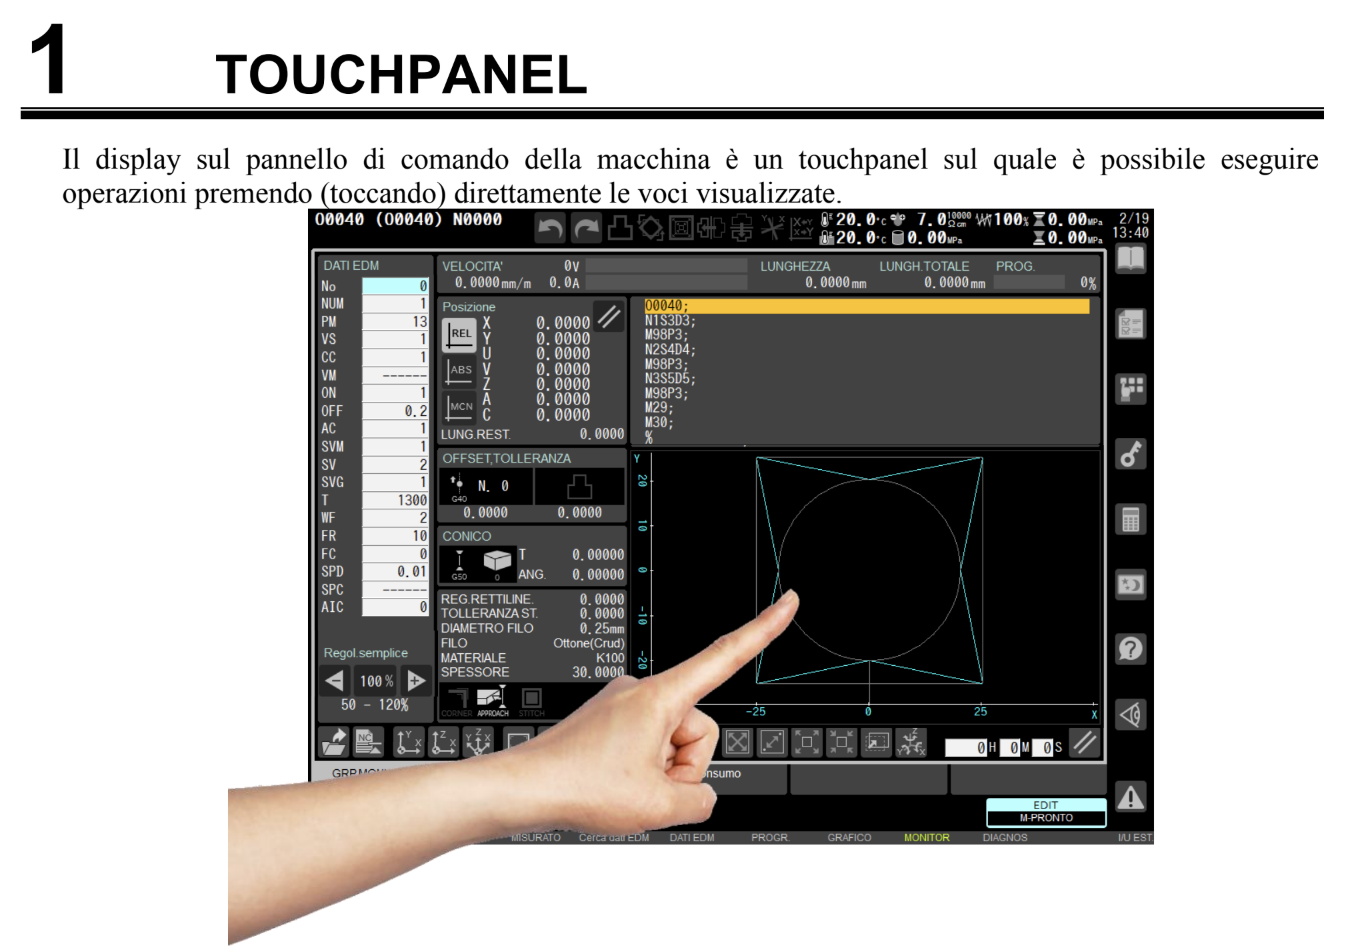
\includegraphics[width=2.5cm,height=1.7cm,keepaspectratio]{figure/asset/touch-panel-schermata-operatore.png}};
\pic[scale=0.7] at (13.25,-1.35) {documento-strutturato};
\node[schema etichetta,text width=2.8cm] at (9.8,-2.7) {\textbf{Ritaglio originale}};
\node[schema etichetta,text width=3.7cm] at (13.25,-2.7)
  {Manuale, pagina ed eventuale caption originale};
\pic[scale=0.67] at (9.4,-4.35) {frammenti};
\node[schema etichetta,text width=3.8cm] at (12.95,-4.35)
  {\textbf{Contesto selezionato}\\Al massimo 6 elementi\\e 2400 caratteri};
\draw[schema freccia] (7,-4.35) -- (8.55,-4.35);
\node[schema nota,text width=6.5cm] at (11.8,-5.45)
  {Il testo serve a disambiguare il visibile.};
\node[schema oggetto,minimum width=2.2cm,minimum height=1.8cm] (vlm) at (9.3,-7.4) {};
\pic[scale=0.8] at (9.3,-7.4) {modello};
\node[schema oggetto,minimum width=2.5cm,minimum height=1.8cm] (descrizione) at (13.1,-7.4) {};
\pic[scale=0.85] at (13.1,-7.4) {dialogo};
\draw[schema freccia] (9.3,-5.95) -- (vlm.north);
\draw[schema freccia] (vlm.east) -- (descrizione.west);
\node[schema etichetta,text width=2.2cm] at (9.3,-8.75) {\textbf{VLM}};
\node[schema etichetta,text width=4.5cm] at (13.1,-8.75)
  {\textbf{Descrizione generata}\\Da confrontare con la fonte};
\pic[scale=0.58] at (0.9,-7.95) {dialogo};
\draw[schemaOcra,line width=1.5pt,line cap=round] (0.25,-8.45) -- (1.55,-7.45);
\node[schema etichetta,anchor=west,align=left,text width=4.8cm] at (2,-8.05)
  {\textbf{Nessun riuso come fonte}\\Le descrizioni generate non entrano nel contesto delle figure successive.};
\end{tikzpicture}
\caption{Composizione degli ingressi del captioning. Le fonti testuali seguono un ordine di priorità, non vengono sommate indiscriminatamente; in assenza di fonti ammissibili, la richiesta non contiene contesto né percorso strutturale. La miniatura dai materiali FANUC forniti è illustrativa, non un risultato del captioning. La descrizione generata va confrontata con la fonte e non diventa una nuova fonte per le richieste successive.}
\label{fig:contesto-caption}
\end{figure}

Il prompt richiede sette campi: \emph{Tipo tecnico}, \emph{Oggetto}, \emph{Elementi visibili}, \emph{Relazioni/funzione}, \emph{Valori/avvertenze}, \emph{Rilevanza RAG} e \emph{Incertezze}. La descrizione deve rimanere entro 1200 caratteri e l'elenco visuale è limitato a otto elementi unici. Le istruzioni impongono di basarsi sul contenuto visibile, di usare il contesto soltanto per disambiguare nomi e sigle, e di dichiarare esplicitamente letture non possibili. Il campo \emph{Rilevanza RAG} richiede una domanda operativa breve, non una misura del recupero. Questi vincoli circoscrivono formato e lunghezza, ma il loro rispetto non prova la fedeltà alla figura. In particolare, il tetto di otto elementi può comprimere eccessivamente tavole esplose o interfacce dense, e quello di 1200 caratteri può escludere una risposta indipendentemente dalla sua qualità informativa.

La scelta finale è il risultato di iterazioni documentate, non di una ricerca di iperparametri su un insieme di test indipendente. Le prove esplorative del settembre 2026 non hanno motivato l'adozione di prompt più lunghi; V3 ha mantenuto il testo del prompt precedente e introdotto controlli aggiuntivi sulle descrizioni. Il successivo ciclo V4 ha escluso le tabelle dalle richieste al VLM, rivisto il contesto delle figure OCR e reso non bloccanti gli errori delle singole caption. Le prove V2 con Ollama \texttt{0.31.2}, le prove intermedie su \texttt{0.33.3} e il ciclo finale su \texttt{0.34.0} devono restare distinti: l'accettazione di un setup storico non si trasferisce automaticamente a quello successivo.

Prima dei controlli, il provider normalizza gli spazi e rimuove le righe vuote della risposta: il limite di lunghezza riguarda il testo normalizzato, non il corpo HTTP grezzo. La risposta viene quindi controllata per formato e lunghezza; alcuni casi richiedono inoltre revisione. Le descrizioni di schemi elettrici e quelle con determinate contraddizioni tra letture incerte e dichiarazioni di assenza di incertezza ricevono lo stato \texttt{review\_required}. La caption viene conservata, ma l'elemento è escluso dall'uso RAG previsto. Un errore di generazione o validazione produce invece \texttt{failed} per l'elemento e una motivazione di esclusione. Gli altri esiti sono \texttt{enriched} e \texttt{skipped}. Il fallimento di una singola caption non coincide necessariamente con l'interruzione dell'intera run.

La provenienza registra provider, modello, versione del prompt, parametri e versione del runtime, oltre a un hash costruito dalla richiesta e dall'asset. È quindi possibile controllare se la descrizione è ancora coerente con gli ingressi documentati. L'hash non certifica che le affermazioni generate siano vere: identifica l'ingresso, non la correttezza semantica dell'uscita.

\subsection{Serializzazione deterministica delle tabelle}

Il modulo \texttt{table\_serialization.py} applica la strategia \texttt{header\_value\_rows\_v1}. Interpreta il contenuto del campo \texttt{table\_markdown}, che può includere rappresentazioni Markdown o HTML, e produce righe testuali con associazioni intestazione--valore. Alla riga vengono aggiunti riferimenti contestuali al manuale, al percorso di capitolo, alla pagina e alla tabella. Non vengono creati chunk né embedding: si prepara una rappresentazione tabellare utilizzabile da componenti successive.

Lo stato \texttt{structured} indica che sono state ottenute righe strutturate; \texttt{fallback} conserva in un'unica riga il contenuto normalizzato quando la struttura non è interpretabile; \texttt{unavailable} indica l'assenza di contenuto tabellare testuale utilizzabile. Quest'ultimo caso può verificarsi anche quando esiste un ritaglio della tabella. La serializzazione non può recuperare valori che il parser non ha acquisito e non usa il VLM per completarli. Mantenere separati questi stati evita di equiparare una tabella trascritta con relazioni esplicite a una semplice conservazione del testo grezzo.

La Figura~\ref{fig:trattamento-visuale} mette a confronto il percorso generativo delle immagini e quello deterministico delle tabelle, mantenendo distinti i rispettivi esiti.

\begin{figure}[!htbp]
\centering
\begin{tikzpicture}[schema base]
\node[schema esterno,text width=13.7cm] at (7.5,0)
  {\textbf{Filtro geometrico comune dopo l'assemblaggio}\\$\rho<0{,}02$: esclusione dall'uso previsto, non cancellazione dell'asset};
\node[schema titolo] at (0.3,-1.3) {Immagini: interpretazione generativa};
\node[schema titolo] at (8.1,-1.3) {Tabelle: trasformazione deterministica};
\draw[schema separatore,draw=schemaGrigio!55] (7.5,-1.6) -- (7.5,-8.55);
\node[schema oggetto,minimum width=4.2cm,minimum height=2.5cm] (immagine) at (3.3,-2.85) {};
\node[inner sep=0pt] at (3.3,-2.6)
  {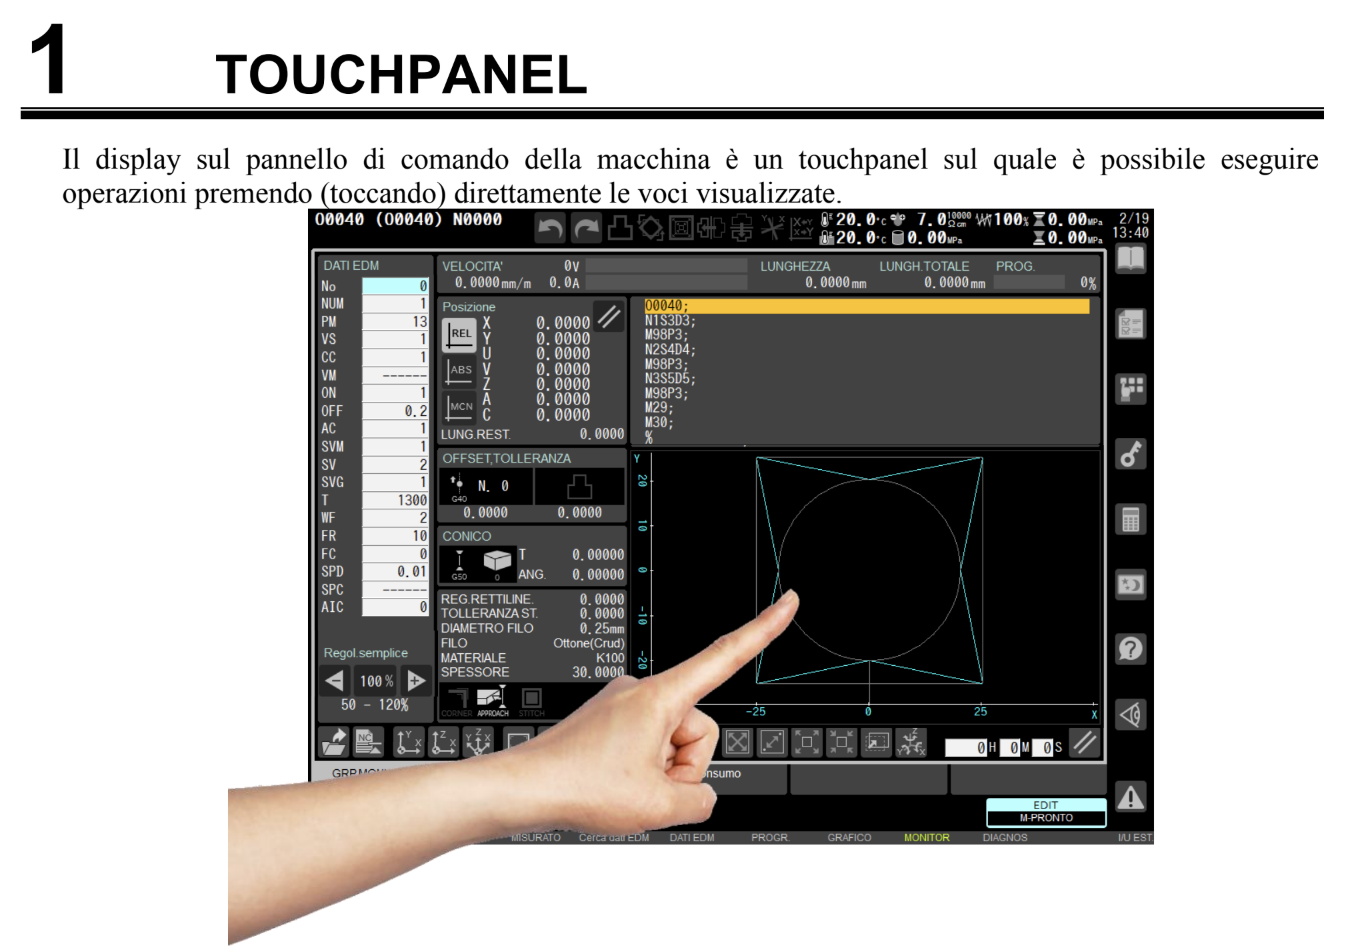
\includegraphics[width=3.7cm,height=2.15cm,keepaspectratio]{figure/asset/touch-panel-schermata-operatore.png}};
\node[schema nota,text width=6cm] at (3.3,-4.05) {Ritaglio ammissibile\\+ eventuale contesto sorgente};
\node[schema oggetto,minimum height=2.5cm] (tabella) at (11.7,-2.85) {};
\pic[scale=1.8] at (11.7,-2.6) {tabella};
\node[schema nota,text width=6cm] at (11.7,-4.05) {Contenuto testuale acquisito\\in Markdown o HTML};
\node[schema oggetto,minimum height=1.5cm] (caption) at (3.3,-5.65) {};
\pic[scale=0.72] at (2.35,-5.65) {modello};
\pic[scale=0.65] at (4.5,-5.65) {dialogo};
\draw[schema freccia] (3.1,-5.65) -- (3.73,-5.65);
\node[schema etichetta,text width=6.1cm] at (3.3,-7.55)
  {\textbf{Captioning con VLM}\\Controlli di formato e lunghezza;\\accettazione, revisione o errore.\\La fedeltà richiede verifica sulla fonte.};
\node[schema oggetto,minimum height=1.5cm] (righe) at (11.7,-5.65) {};
\foreach \ordinata/\colore in {-5.12/schemaBlu,-5.65/schemaVerde,-6.18/schemaOcra} {
  \path[schema icona,draw=\colore,fill=\colore!12] (9.5,\ordinata-0.19) rectangle (13.9,\ordinata+0.19);
  \node[font=\ttfamily\footnotesize] at (11.7,\ordinata) {intestazione: valore};
}
\node[schema etichetta,text width=6.1cm] at (11.7,-7.55)
  {\textbf{Serializzazione delle righe}\\Righe con contesto, testo di ripiego\\o contenuto non disponibile.\\Nessun valore non acquisito viene ricostruito.};
\draw[schema freccia] (3.3,-4.55) -- (caption.north);
\draw[schema freccia] (11.7,-4.55) -- (righe.north);
\end{tikzpicture}
\caption{Trattamento delle immagini e delle tabelle nel workflow corrente; le colonne non indicano esecuzione parallela. Schermata del manuale FANUC dai materiali forniti come esempio visuale, non risultato del captioning; tabella e righe sono schematiche. Le tabelle non vengono inviate al VLM e sono serializzate anche se escluse dall'uso previsto, senza annullare tale esclusione.}
\label{fig:trattamento-visuale}
\end{figure}

\section{Output, tracciabilità e controlli della pipeline}
\label{sec:output-controlli}

\subsection{Artefatti e pubblicazione atomica}

La Tabella~\ref{tab:run-bundle} distingue il documento canonico dagli asset, dai metadati e dalle evidenze di controllo conservati nel bundle.

\begin{table}[!htbp]
\centering
\caption{Artefatti del run bundle nella configurazione ordinaria.}
\label{tab:run-bundle}
\small
\begin{tabularx}{\textwidth}{@{}p{0.27\textwidth}X@{}}
\toprule
Artefatto & Contenuto \\
\midrule
\texttt{manual.json} & Documento canonico: gerarchia, elementi, riferimenti agli asset, descrizioni e tracce. \\
\texttt{toc.json} & Lista delle voci di indice con titolo, livello, pagina ed eventuale confidenza. Non è un indice RAG. \\
\texttt{run.json} & Manifest: identità e stato della run, sorgente e hash, configurazione, capacità rilevate, percorsi, tempi, avvisi ed errori. \tabularnewline
\texttt{validation.json} & Esito dei controlli, messaggi e metriche tecniche; è richiesto nei bundle finali validati o sperimentali. \\
\texttt{assets/} & Rendering e ritagli effettivamente prodotti dagli adattatori. \\
\texttt{diagnostics/} & Evidenze di detection, struttura, filtro, enrichment, runtime e promozione; ulteriori artefatti del percorso OCR. \\
\bottomrule
\end{tabularx}
\end{table}

\texttt{RunBundleWorkspace}, definito in \texttt{run\_bundle.py}, mantiene gli artefatti in una directory di staging sullo stesso filesystem della destinazione. La pubblicazione avviene tramite rinomina dopo il completamento dei controlli. Una destinazione già esistente viene rifiutata, così da non sovrascrivere una run precedente. In caso di errore prima della pubblicazione, lo staging viene rimosso: un insieme incompleto di file non viene presentato come bundle finale.

Il sorgente è identificato mediante nome, dimensione e SHA-256; l'orchestratore verifica che non cambi durante l'elaborazione. I percorsi degli artefatti devono rimanere relativi e non attraversare directory superiori. La diagnostica comune comprende \texttt{detection.json}, \texttt{structure.json}, \texttt{crop\_filter.json}, \texttt{enrichment.json}, \texttt{runtime.json} e \texttt{promotion.json}. Il manifest e la diagnostica registrano configurazioni e versioni necessarie a interpretare la run, ma la riproduzione richiede anche di conservare il PDF identificato e rendere disponibile il runtime corrispondente.

La Figura~\ref{fig:flusso-pubblicazione} segue il passaggio dallo staging al bundle finale e distingue un impedimento alla promozione da un errore che interrompe l'esecuzione. È una vista operativa complementare ai tre piani di verifica della Figura~\ref{fig:livelli-verifica}.

\begin{figure}[!htbp]
\centering
\begin{tikzpicture}[schema base]
\node[schema oggetto,minimum width=2.2cm,minimum height=1.6cm] (inizio) at (1.3,0) {};
\pic[scale=0.76] at (1.3,0) {fascicolo};
\node[schema etichetta,align=left,text width=5.8cm] at (5.85,0)
  {\textbf{Staging: file provvisori}\\Controlli preliminari e detection;\\creazione dello staging\\ed elaborazione};
\node[schema oggetto,minimum width=2.2cm,minimum height=1.6cm] (bozza) at (1.3,-2.5) {};
\pic[scale=0.76] at (1.3,-2.5) {controllo-fonte};
\node[schema etichetta,align=left,text width=5.8cm] (testobozza) at (5.85,-2.5)
  {\textbf{Verifica della bozza}\\Valutazione della promozione;\\scrittura e validazione della bozza};
\node[schema oggetto,minimum width=2.2cm,minimum height=1.6cm] (stato) at (1.3,-5) {};
\pic[scale=0.86] at (1.3,-5) {testo};
\node[schema etichetta,align=left,text width=5.8cm] at (5.85,-5)
  {\textbf{Assegnazione dello stato finale}\\Requisiti soddisfatti: \texttt{validated}\\Impedimenti: \texttt{experimental}};
\node[schema oggetto,minimum width=2.2cm,minimum height=1.6cm] (finale) at (1.3,-7.5) {};
\pic[scale=0.86] at (1.3,-7.5) {checklist};
\node[schema etichetta,align=left,text width=5.8cm] (testofinale) at (5.85,-7.5)
  {\textbf{Controlli finali}\\Manifest finale e report ricalcolato;\\controlli e integrità del sorgente};
\node[schema oggetto,minimum width=2.2cm,minimum height=1.6cm] (pubblicazione) at (1.3,-10) {};
\pic[scale=0.76] at (1.3,-10) {fascicolo};
\path[fill=schemaCartaVerde,draw=schemaVerde] (2.12,-10.42) circle (0.28);
\draw[schemaVerde,line width=1.25pt] (1.96,-10.43) -- (2.07,-10.53) -- (2.29,-10.3);
\node[schema etichetta,align=left,text width=5.8cm] at (5.85,-10)
  {\textbf{Pubblicazione mediante rinomina}\\Bundle \texttt{validated}\\o \texttt{experimental}};
\draw[schema freccia] (inizio) -- (bozza);
\draw[schema freccia] (bozza) -- node[right,schema nota] {Bozza valida} (stato);
\draw[schema freccia] (stato) -- (finale);
\draw[schema freccia] (finale) -- node[right,schema nota] {Controlli superati} (pubblicazione);
\node[schema oggetto,minimum height=1.6cm] (errore) at (12.15,-6) {};
\pic[scale=0.95] at (12.15,-6) {cartella};
\draw[schemaOcra,line width=1.7pt,line cap=round] (11.65,-6.43) -- (12.65,-5.6) (11.65,-5.6) -- (12.65,-6.43);
\node[schema etichetta,text width=4.7cm] at (12.15,-7.65)
  {\textbf{Interruzione}\\Nessun nuovo bundle finale.\\Staging rimosso, se creato.};
\draw[schema freccia] (testobozza.east) -- node[above,schema nota] {Bozza non valida} (15,-2.5) |- (errore.east);
\draw[schema freccia] (testofinale.east) -- (9.65,-7.5) |- node[pos=0.8,above,schema nota] {Errore} (errore.west);
\node[schema nota,text width=4.7cm] at (12.15,-4.2)
  {Anche altri errori fatali possono interrompere il flusso prima della rinomina.};
\node[schema nota,text width=4.7cm] at (12.15,-10)
  {Un errore locale di captioning può essere registrato senza bloccare la pubblicazione.};
\end{tikzpicture}
\caption{Pubblicazione secondo \texttt{orchestrator.py} e \texttt{run\_bundle.py}: dal fascicolo provvisorio a quello pubblicato, oppure all'interruzione. Il segno di spunta indica la pubblicazione, non necessariamente lo stato \texttt{validated}. La conformità tecnica permette di pubblicare; la politica di promozione determina lo stato. I file nello staging sono provvisori fino alla rinomina.}
\label{fig:flusso-pubblicazione}
\end{figure}

\subsection{Validazione tecnica e politica di promozione}

Il validatore in \texttt{validation.py} ricostruisce un report a partire dagli artefatti, invece di fidarsi dell'esito già salvato. Il report dichiarato deve corrispondere a quello ricalcolato; una fingerprint del bundle contribuisce a rilevare modifiche. I controlli riguardano esistenza e schema dei file, coerenza degli identificativi e del sorgente, limiti delle pagine, unicità degli ID, relazioni padre--figlio, percorsi ed esistenza degli asset, provenienza delle caption, struttura della TOC, serializzazione tabellare ed evidenze di promozione.

Un controllo specifico impone che gli elementi canonici coprano almeno il 75\% delle pagine dichiarate elaborate. Indicando con $P$ l'insieme delle pagine elaborate e con $E$ quello delle pagine contenenti almeno un elemento, il requisito è
\begin{equation}
    |E\cap P|\geq\left\lceil0{,}75|P|\right\rceil.
\end{equation}
Questa soglia è distinta da quella usata nella detection: la prima riguarda il risultato del parsing, la seconda il campione testuale di ingresso. Nessuna delle due dimostra che ogni contenuto di una pagina sia stato acquisito, né che tutte le pagine prive di elementi siano effettivamente vuote.

La validazione controlla anche il setup software rispetto alle versioni accettate nella politica implementata. Nelle due run V4 sono registrati Python \texttt{3.12.13}, \texttt{manual\_ingestion 1.0.0}, Pydantic \texttt{2.13.4}, PyMuPDF \texttt{1.28.0} e Pillow \texttt{11.3.0}; la run digitale registra inoltre Docling \texttt{2.112.0}, quella OCR le versioni Paddle indicate nella Sezione~\ref{sec:profili}. Queste identità sono riscontrabili nei manifest e nella diagnostica, ma la versione del pacchetto non identifica da sola ogni revisione dei sorgenti. Il diario riferisce una postazione M1 Max con 32 GB per lo sviluppo; gli artefatti finali non contengono un inventario hardware sufficiente a trattare le durate registrate come un benchmark prestazionale riproducibile su quella configurazione.

La promozione è definita separatamente in \texttt{promotion.py}. Per dichiarare una run \texttt{validated} non basta che il JSON sia leggibile: occorrono copertura dell'intero documento, enrichment conforme, identità coerenti delle caption, assenza di casi che richiedono revisione, assenza di avvisi impeditivi, accettazione del profilo e struttura compatibile con la politica. Per l'OCR la politica registra un identificativo di evidenza di accettazione e distingue la ricostruzione mediante indice dal ripiego sui soli titoli. Nel caso dell'indice stampato OCR, la promozione richiede la risoluzione del 100\% delle righe: la soglia dell'80\% consente alla ricostruzione di proseguire, ma non basta per dichiarare la run validata.

Occorre quindi distinguere tre piani:
\begin{description}
    \item[Conformità tecnica.] Il report assume \texttt{passed} soltanto se tutti i controlli previsti sono superati.
    \item[Stato della run.] Una run tecnicamente coerente è \texttt{experimental} se non soddisfa i requisiti di promozione; è \texttt{validated} quando li soddisfa. Un report \texttt{passed} è compatibile con uno stato \texttt{experimental} correttamente motivato.
    \item[Correttezza semantica.] La fedeltà di testi, gerarchia, ritagli e descrizioni alla fonte richiede un confronto documentale distinto. Non è dimostrata dal nome \texttt{validated}.
\end{description}

I contratti definiscono anche \texttt{incomplete}, \texttt{completed} e \texttt{failed}; il percorso ordinario usa \texttt{completed} per il manifest provvisorio e pubblica l'esito finale soltanto dopo la verifica. Un errore fatale non produce normalmente un bundle finale con stato \texttt{failed}. La CLI può invece scrivere, mediante \texttt{--write-failure-report}, un report compatto accanto alla destinazione, con il contesto dell'interruzione. È quindi necessario raccogliere anche tali esiti quando si valuta la robustezza, evitando di considerare soltanto i bundle pubblicati.

La Figura~\ref{fig:livelli-verifica} riassume la separazione tra conformità tecnica, promozione della run e fedeltà dei contenuti alla fonte. Questa distinzione orienta il metodo di valutazione descritto nel seguito.

\begin{figure}[!htbp]
\centering
\begin{tikzpicture}[schema base]
\node[schema etichetta,text width=14.5cm] at (7.5,1.35)
  {\textbf{Tre domande distinte, non una scala di avanzamento}};
\pic[scale=0.86] at (1.15,0) {checklist};
\node[schema etichetta,anchor=west,align=left,text width=4.35cm] (tecnica) at (2.35,0)
  {\textbf{Conformità tecnica}\\Gli artefatti rispettano il contratto?};
\path[schema icona,fill=white]
  (8.6,-0.82) -- (14.8,-0.82) -- (14.8,0.47) -- (14.45,0.82) -- (8.6,0.82) -- cycle;
\draw[schema icona] (14.45,0.82) -- (14.45,0.47) -- (14.8,0.47);
\node[schema etichetta,text width=5.5cm] (report) at (11.7,0)
  {\textbf{Report} \texttt{passed}\\Tutti i controlli previsti superati};
\draw[schema freccia] (tecnica.east) -- (8.55,0);
\draw[schemaGrigio!45,dash pattern=on 3pt off 4pt,line width=0.65pt] (0,-1.4) -- (15,-1.4);
\pic[scale=0.72] at (1.15,-2.8) {fascicolo};
\node[schema etichetta,anchor=west,align=left,text width=4.35cm] (politica) at (2.35,-2.8)
  {\textbf{Promozione}\\La run soddisfa la politica?};
\node[schema blocco,draw=schemaVerde,fill=schemaCartaVerde,text width=3.5cm,minimum height=0.7cm,inner sep=5pt] (validated) at (12.1,-2.25)
  {\texttt{validated}};
\node[schema esterno,text width=3.5cm,minimum height=0.7cm,inner sep=5pt] (experimental) at (12.1,-3.35)
  {\texttt{experimental}};
\draw[schemaInchiostro,line cap=round] (politica.east) -- (8.25,-2.8);
\draw[schema freccia] (8.25,-2.8) |- node[pos=0.75,above,schema nota] {Sì} (validated.west);
\draw[schema freccia] (8.25,-2.8) |- node[pos=0.75,above,schema nota] {No} (experimental.west);
\draw[schemaGrigio!45,dash pattern=on 3pt off 4pt,line width=0.65pt] (0,-4.25) -- (15,-4.25);
\pic[scale=0.62] at (0.65,-5.7) {pagina};
\pic[scale=0.7] at (1.55,-5.85) {testo};
\draw[schemaBlu,line width=1.15pt] (1.2,-5.65) circle (0.3);
\draw[schemaBlu,line width=1.8pt,line cap=round] (1.42,-5.87) -- (1.78,-6.23);
\node[schema etichetta,anchor=west,align=left,text width=4.35cm] (semantica) at (2.35,-5.7)
  {\textbf{Correttezza semantica}\\Contenuti e associazioni sono fedeli?};
\node[schema etichetta,text width=6.2cm] (fonte) at (11.7,-5.7)
  {\textbf{Confronto documentale con la fonte}\\Non deducibile dagli stati automatici};
\draw[schema freccia] (semantica.east) -- (fonte.west);
\end{tikzpicture}
\caption{Tre domande distinte, non tre tappe equivalenti. La checklist riguarda i controlli tecnici, il fascicolo lo stato della run e la lente il confronto con la fonte. Un report \texttt{passed} è compatibile con una run \texttt{experimental}; nessuno dei due stati dimostra la correttezza semantica.}
\label{fig:livelli-verifica}
\end{figure}

\section{Metodo di valutazione}
\label{sec:valutazione}

La valutazione combina verifica software, prove documentali per profilo e analisi descrittiva dell'enrichment. Non è un benchmark pubblico di parser né uno studio di efficacia del RAG. Le prove complete e le selezioni visuali rispondono a domande diverse: le prime verificano la produzione di una rappresentazione coerente su un intero input; le seconde rendono ispezionabili richieste, informazioni aggiunte ed errori del modello. I test, la matrice di accettazione e le registrazioni finali documentano questo disegno, mantenendo distinta l'evidenza direttamente verificabile da quella conservata soltanto nei report.

La Figura~\ref{fig:metodo-valutazione} organizza le sottosezioni seguenti in un fondamento trasversale e tre assi complementari. La sintesi evita di trattare come fasi consecutive attività che rispondono a domande diverse e usano evidenze differenti.

\begin{figure}[!htbp]
\centering
\begin{tikzpicture}[
  schema base,
  schema asse/.style={schema blocco,minimum width=4.65cm,minimum height=4.9cm,inner sep=8pt},
  schema unita/.style={schema blocco,fill=white,minimum width=1.5cm,minimum height=0.58cm,inner sep=3pt,font=\schemafont\footnotesize},
  schema numero/.style={circle,text=white,font=\schemafont\footnotesize\bfseries,minimum size=7mm,inner sep=0pt},
  schema corpo/.style={font=\schemafont\scriptsize,align=left,text=schemaInchiostro},
  schema rq/.style={circle,draw=schemaBlu,fill=schemaCartaBlu,font=\schemafont\footnotesize\bfseries,minimum size=8mm,inner sep=1pt}
]
\node[schema titolo] at (0,0.45) {Metodo di valutazione: un fondamento comune e tre assi di analisi};

% Fondamento trasversale: definisce che cosa viene contato e dove resta la prova.
\node[schema pannello,minimum width=15cm,minimum height=1.9cm] (fondamento) at (7.5,-0.8) {};
\node[schema numero,fill=schemaBlu] at (0.55,-0.25) {0};
\node[schema titolo] at (0.95,-0.25) {Unità di analisi e registrazioni trasversali};
\node[schema unita] (documento) at (1.25,-1.12) {Documento};
\node[schema unita] (run) at (3.05,-1.12) {Run};
\node[schema unita] (voce) at (4.85,-1.12) {Voce};
\node[schema unita] (elemento) at (6.65,-1.12) {Elemento};
\draw[schema freccia] (documento.east) -- (run.west);
\draw[schema freccia] (run.east) -- (voce.west);
\draw[schema freccia] (voce.east) -- (elemento.west);
\node[schema corpo,anchor=west] at (8.25,-1.02) {%
  \textbf{Tracce conservate}\\
  \texttt{run.json}, snapshot, eventi e asset\\
  richieste e risposte in \texttt{evidence}};

% Tre assi che raggruppano le restanti sottosezioni.
\node[schema asse,draw=schemaVerde,fill=schemaCartaVerde!45] (pipeline) at (2.35,-4.95) {};
\node[schema numero,fill=schemaVerde] at (0.55,-2.95) {1};
\node[schema etichetta,text width=3.6cm] at (2.65,-3.05) {\textbf{Pipeline e struttura}};
\draw[schema tratto,draw=schemaVerde!55] (0.35,-3.55) -- (4.35,-3.55);
\node[schema corpo,anchor=north west] at (0.65,-3.85) {%
  \textbf{Verifica software}\\
  Test e prove di accettazione\\[7pt]
  \textbf{Rappresentazione comune}\\
  Confronto tra struttura,\\
  output e fonte};

\node[schema asse,draw=schemaBlu,fill=schemaCartaBlu!55] (studio) at (7.5,-4.95) {};
\node[schema numero,fill=schemaBlu] at (5.7,-2.95) {2};
\node[schema etichetta,text width=3.6cm] at (7.8,-3.05) {\textbf{Studio V4 sull'enrichment}};
\draw[schema tratto,draw=schemaBlu!55] (5.5,-3.55) -- (9.5,-3.55);
\node[schema corpo,anchor=north west] at (5.8,-3.85) {%
  \textbf{Disegno V4}\\
  Selezione mirata e campione\\[5pt]
  \textbf{Confronto descrittivo}\\
  Baseline, output e giudizio\\[5pt]
  \textbf{Misure operative}\\
  Esclusioni e denominatori\\
  Durate registrate};

\node[schema asse,draw=schemaOcra,fill=schemaCartaGialla!55] (audit) at (12.65,-4.95) {};
\node[schema numero,fill=schemaOcra] at (10.85,-2.95) {3};
\node[schema etichetta,text width=3.6cm] at (12.95,-3.05) {\textbf{Audit e riproducibilità}};
\draw[schema tratto,draw=schemaOcra!65] (10.65,-3.55) -- (14.65,-3.55);
\node[schema corpo,anchor=north west] at (10.95,-3.85) {%
  \textbf{Catena verificata}\\
  Asset e richiesta\\
  Risposta e documento finale\\[7pt]
  \textbf{Integrità e identità}\\
  Hash, fingerprint e sorgenti\\[7pt]
  \textbf{Riproducibilità}\\
  Revisione eseguita\\
  non riproducibile integralmente};

% Il fondamento comune alimenta tutti gli assi; ciascun asse sostiene una RQ.
\coordinate (dorsale-sinistra) at (2.35,-2.08);
\coordinate (dorsale-centro) at (7.5,-2.08);
\coordinate (dorsale-destra) at (12.65,-2.08);
\draw[schema tratto,draw=schemaInchiostro,line width=0.8pt]
  (fondamento.south) -- (dorsale-centro);
\draw[schema tratto,draw=schemaInchiostro,line width=0.8pt]
  (dorsale-sinistra) -- (dorsale-destra);
\fill[schemaInchiostro] (dorsale-sinistra) circle (1.15pt);
\fill[schemaInchiostro] (dorsale-centro) circle (1.15pt);
\fill[schemaInchiostro] (dorsale-destra) circle (1.15pt);
\draw[schema freccia] (dorsale-sinistra) -- (pipeline.north);
\draw[schema freccia] (dorsale-centro) -- (studio.north);
\draw[schema freccia] (dorsale-destra) -- (audit.north);

\node[schema rq] (rqone) at (2.35,-8.1) {RQ1};
\node[schema rq] (rqtwo) at (7.5,-8.1) {RQ2};
\node[schema rq] (rqthree) at (12.65,-8.1) {RQ3};
\draw[schema freccia] (pipeline.south) -- (rqone.north);
\draw[schema freccia] (studio.south) -- (rqtwo.north);
\draw[schema freccia] (audit.south) -- (rqthree.north);
\end{tikzpicture}
\caption{Organizzazione del metodo di valutazione. Le unità e le registrazioni sono trasversali; le altre sottosezioni confluiscono in tre assi complementari, rispettivamente collegati alla rappresentazione comune, all'enrichment V4 e alla verificabilità degli artefatti.}
\label{fig:metodo-valutazione}
\end{figure}
\FloatBarrier

\subsection{Unità di analisi e registrazione delle esecuzioni}

Si distinguono quattro unità: documento, run, voce gerarchica ed elemento. Il documento identifica la fonte; la run identifica una particolare elaborazione e configurazione; la voce gerarchica consente di verificare titolo, livello, destinazione e relazione con il padre; l'elemento consente di controllare acquisizione, appartenenza, asset ed eventuali informazioni derivate. Ripetizioni o prove parziali sullo stesso PDF non devono essere conteggiate come documenti indipendenti.

Per le run V4 questi dati sono conservati in \texttt{run.json}, \texttt{validation.json} e nella directory \texttt{evidence}. Quest'ultima registra comando e argomenti effettivi, configurazione del provider, esito della CLI, eventi temporali, chiamate di enrichment e scambi HTTP. Le snapshot \texttt{manual-before.json} e \texttt{manual-after.json} delimitano la trasformazione generativa; l'inventario degli asset e gli hash consentono di collegare la richiesta al ritaglio effettivamente inviato. Il conteggio delle chiamate proviene dalle registrazioni, non dal solo numero di caption presenti nel documento finale.

Le esecuzioni senza provider e quelle su un sottoinsieme delle pagine restano identificate come diagnostiche. L'unità per descrivere l'esito della pipeline è il tentativo di esecuzione, inclusi eventuali fallimenti senza pubblicazione; l'unità per descrivere il captioning è la singola richiesta al provider. Gli esiti delle prove esplorative V3 non sono aggregati a quelli del ciclo V4: il comportamento sugli errori e il trattamento delle tabelle sono cambiati. L'archivio V4 documenta due tentativi, non il totale di tutte le prove svolte durante lo sviluppo.

\subsection{Verifica software e prove di accettazione}

La directory \texttt{tests} contiene 22 moduli di test. La loro funzione è verificare contratti e transizioni osservabili, anche con PDF sintetici, provider simulati e risposte OCR controllate; non attribuire accuratezza semantica ai motori reali. La Tabella~\ref{tab:test-metodi} riassume le aree pertinenti al metodo. La matrice storica registra una suite di 329 test superati per il rilascio allora verificato: quel conteggio non viene trasferito automaticamente allo stato dei sorgenti qui archiviati, né presentato come una nuova esecuzione della suite.

\begin{table}[!htbp]
\centering
\caption{Copertura funzionale dei test in \texttt{tesi-di-nardo/tests}, distinta dalla verifica semantica del corpus.}
\label{tab:test-metodi}
\small
\begin{tabularx}{\textwidth}{@{}>{\raggedright\arraybackslash}p{0.25\textwidth}X@{}}
\toprule
Area & Comportamenti verificati dai test presenti \\
\midrule
Detection e profili & Routing, input inutilizzabili, scelta del parser e rifiuto di override incoerenti. \tabularnewline
Struttura & Offset, indice multipagina, titoli lunghi o duplicati, limiti di pagina, ancoraggi locali e ricostruzione OCR. \tabularnewline
Asset ed enrichment & Percorsi, filtro, fonti immutabili, esclusione delle tabelle dal VLM, provenienza e risposte non conformi. \tabularnewline
Tabelle & Markdown/HTML, celle unite, intestazioni irregolari, fallback e testo assente; purezza, determinismo e idempotenza. \tabularnewline
Orchestrazione e bundle & Pubblicazione atomica, protezione dalla sovrascrittura, integrità, report, promozione e fallimenti. \tabularnewline
\bottomrule
\end{tabularx}
\end{table}

Due test rendono esplicite le scelte finali dell'enrichment: il primo usa un provider che genera un errore se chiamato su una tabella, verificando che la tabella lo salti; il secondo costruisce una pagina con sezioni relative a figure diverse e verifica che il prompt usi soltanto il testo associato alla figura bersaglio. Queste prove isolano il comportamento voluto, ma non stabiliscono quanto spesso il riconoscimento del contesto riesca sui PDF reali. Analogamente, i test della serializzazione verificano la trasformazione delle celle già acquisite, non la correttezza dell'OCR che le ha prodotte.

\subsection{Verifica della rappresentazione comune}

Per il profilo digitale ricostruito il riferimento del confronto è l'outline del PDF gemello. La matrice riporta un confronto su titoli, pagine, ordine e livelli, con una correzione esplicita dell'offset di livello alla radice. Recall e precision dei titoli descrivono copertura e sovrapproduzione rispetto a quel riferimento; la corrispondenza di pagina è distinta fra esatta ed entro una pagina di scarto. Il benchmark riguarda la gerarchia, non misura automaticamente la conservazione del testo o l'associazione delle figure ai capitoli. L'harness di confronto e le corrispondenze elementari non sono inclusi nell'archivio del progetto: i punteggi restano quindi quelli delle prove storiche, senza un nuovo calcolo.

Per l'OCR, la prova integrale documentata considera l'indice stampato a pagina 5 del WM250, lo scarto tra numerazione stampata e pagina fisica e la risoluzione delle relative voci. La matrice descrive anche l'ispezione delle pagine 26 e 33, ruotate di 180 gradi, insieme ai ritagli. Si tratta di verifiche localizzate, non di una trascrizione di riferimento completa del manuale. La run V4 sulle sole pagine 8, 10, 26 e 33 non comprende l'indice a pagina 5 e usa il fallback sui titoli OCR: il suo limite strutturale non va confuso con l'esito del percorso completo mediante indice.

La verifica semantica ha come riferimento la fonte visuale, non il solo JSON. Per gli elementi si distinguono conservazione del testo, completezza del ritaglio, associazione al capitolo e ordine di lettura. Il confronto deve essere bidirezionale: partire dall'output permette di individuare contenuti errati o duplicati, ma solo partire dalla pagina sorgente consente di rilevare omissioni. Poiché l'archivio del progetto non include i PDF integrali, il confronto sui ritagli digitali riguarda le figure conservate e lascia aperta la verifica di eventuali omissioni nelle pagine originarie. Per la selezione OCR sono invece conservati anche i rendering delle quattro pagine.

Le tabelle richiedono un confronto tra celle della fonte, rappresentazione acquisita e righe serializzate. È necessario distinguere errori già introdotti dal parser da errori di serializzazione; il ricalcolo deterministico controlla la seconda trasformazione, non la trascrizione originaria. Analogamente, per le figure bisogna separare ritagli errati, contesti errati e descrizioni errate, poiché si tratta di difetti di stadi differenti.

Le tabelle reali appartengono alle prove storiche complete e alle selezioni delle pagine 3 e 1004, non al campione visuale finale V4. Il confronto riportato nella matrice distingue struttura disponibile, fallback e contenuto testuale assente; non giustifica l'attribuzione di accuratezza cella per cella all'intero corpus. La disponibilità dei test e dei conteggi storici permette di documentare il metodo di serializzazione, senza presentare i due bundle V4, privi di elementi \texttt{table}, come una nuova prova empirica di tale componente.

\subsection{Disegno e campione dello studio finale V4}

Lo studio V4 adotta una selezione mirata e descrittiva di contenuti reali, non un campionamento casuale. Il diario del 15 settembre 2026 stabilisce un ciclo digitale con outline e uno scansionato, senza replicare le immagini digitali nel profilo ricostruito. Le pagine effettivamente elaborate e la popolazione visuale risultante sono ricostruibili dai comandi, dalle snapshot e dai report del filtro, come sintetizzato nella Tabella~\ref{tab:campione-v4}.\footnote{I comandi e gli ingressi effettivi sono conservati nei due file \path{evidence/command.json}; i conteggi sono riscontrabili in \path{bundle/diagnostics/crop_filter.json} e nelle directory \path{evidence/captions}, sotto ciascun caso in \path{tesi-di-nardo/enrichment-v4-final-20260915}.}

\begin{table}[!htbp]
\centering
\caption{Formazione del campione V4: il filtro esclude immagini prima della generazione, non in seguito a errori del VLM. Le selezioni non contengono elementi canonici di tipo tabella.}
\label{tab:campione-v4}
\small
\begin{tabularx}{\textwidth}{@{}>{\raggedright\arraybackslash}p{0.17\textwidth}Xrrr@{}}
\toprule
Caso & Pagine PDF elaborate & Immagini & \shortstack{Escluse\\dal filtro} & Chiamate \tabularnewline
\midrule
Digitale con outline & 73, 93, 98, 225, 228, 352 & 16 & 7 & 9 \\
Scansione WM250 & 8, 10, 26, 33 & 9 & 1 & 8 \\
\midrule
Totale & 10 pagine su due documenti & 25 & 8 & 17 \\
\bottomrule
\end{tabularx}
\end{table}

Il caso digitale è registrato come \path{enrichment-v4-outline-20260915}; quello scansionato come \path{enrichment-v4-scanned-20260915}. Nel digitale il campione comprende uno schema di collegamento elettrico, il touch panel, la tastiera di movimento e schermate o barre di navigazione dell'interfaccia. Nello scansionato comprende fotografie di gruppi meccanici e comandi, oltre a due tavole esplose. Queste classi sono ricavabili dai ritagli; non vengono dedotte dall'etichetta \emph{Tipo tecnico} generata dal modello, che può essere errata.

Le 17 richieste riguardano 17 asset con digest distinti. La selezione mira a rendere osservabili contenuti spaziali, sigle, comandi e relazioni fra figura e testo, senza pretese di rappresentatività statistica dei manuali. Le pagine sono fissate prima delle due esecuzioni documentate, ma provengono da un percorso di sviluppo che ha già utilizzato materiali dello stesso progetto: non costituiscono un insieme di test indipendente dalle scelte di prompt e filtro. Ogni richiesta dispone di una sola risposta nel ciclo archiviato; non sono previste repliche da cui stimare la variabilità della generazione.

\subsection{Baseline e confronto descrittivo}

La baseline è la rappresentazione acquisita prima dell'enrichment: testo della pagina, eventuale \texttt{caption\_original}, collegamenti documentali e asset. Non è una risposta di un sistema RAG alternativo. Nelle nove immagini digitali inviate al modello la caption originale è assente, ma esiste testo contestuale nelle pagine; nelle immagini OCR possono essere già presenti sigle o frammenti di testo riconosciuti. La baseline comprende quindi anche informazioni testuali sulla figura disponibili al di fuori della caption originale. La snapshot \texttt{manual-before.json} e il prompt effettivo permettono di distinguere ciò che è già disponibile da ciò che viene aggiunto dalla lettura visuale.

Il confronto descrittivo documentato nel diario affianca originale, baseline, output Qwen e giudizio breve. Nella valutazione si distinguono: aggiunte visuali supportate dalla fonte; ripetizioni di informazioni già disponibili; omissioni; dettagli o relazioni non supportati; letture errate di sigle e valori; dichiarazioni di incertezza. Non vengono introdotti punteggi di qualità aggregati né un beneficio netto presunto. Le registrazioni tecniche consentono di ricostruire i primi tre termini del confronto; le schede qualitative curate richiamate dal diario non sono comprese nell'archivio del progetto. La documentazione conservata non specifica un protocollo di annotazione indipendente con numero di revisori, accordo inter-annotatore o risoluzione dei disaccordi.

Una caption più lunga o accettata dal validatore non è, per questo, migliore. Analogamente, \texttt{review\_required} è l'esito di una regola automatica che segnala la necessità di controllo, non la prova che un revisore umano sia intervenuto. Per separare i livelli di errore, l'analisi distingue ritaglio sbagliato, contesto non pertinente e interpretazione inesatta di un ingresso corretto. Un'informazione presente nel contesto ma non visibile può spiegare l'uscita del modello senza renderla una lettura fedele della figura.

\subsection{Esclusioni, denominatori e misure operative}

I denominatori dipendono dallo stadio. Per descrivere il filtro si considerano tutte le 25 immagini acquisite; per descrivere la generazione si considerano le 17 chiamate effettive, comprese quelle la cui risposta non entra nel documento finale. Le immagini escluse prima della chiamata, quelle fallite e quelle da rivedere devono rimanere categorie separate. La conservazione degli scarti consente di valutare anche informazione utile eventualmente sottratta all'uso successivo, anziché limitarsi ai casi accettati.

Le risposte oltre il limite di lunghezza sono conservate in \texttt{caption-response.json} e nei corpi delle risposte HTTP anche quando \texttt{caption\_generated} resta vuoto nel documento. Limitare la revisione alle sole caption finali introdurrebbe quindi una selezione favorevole degli esiti. Viceversa, le caption da rivedere possono rimanere nel documento ma con \texttt{include\_in\_rag=false}, che ne mantiene esplicita l'esclusione dall'uso previsto.

Gli eventi e i file \texttt{call.json} distinguono durata della CLI, durata dell'enrichment e durata delle richieste al provider. Un tempo totale include anche acquisizione, rendering, controlli e registrazione degli artefatti; non può essere attribuito integralmente al modello. Le durate disponibili descrivono due esecuzioni strumentate, con diverso numero di pagine e parser: non supportano confronti di velocità fra motori né stime di throughput generalizzabili. Gli esiti operativi e gli esempi di contenuto sono destinati al Capitolo~\ref{cap:risultati}, mantenendo separati metodo e risultati.

\subsection{Audit degli artefatti e limiti di riproducibilità}
\label{sec:audit-metodi}

L'audit dei materiali V4 verifica la catena \emph{asset--richiesta--risposta--documento}. Per ciascuna chiamata sono confrontati il digest del ritaglio, quello dell'immagine codificata nel corpo HTTP e il prompt salvato. Per le caption dotate di provenance si ricostruisce l'hash dall'identificativo dell'elemento, dal tipo, dal prompt e dai byte dell'asset. Si controllano inoltre gli inventari delle immagini e la corrispondenza fra snapshot dopo l'enrichment e documento finale. Poiché i due campioni non contengono tabelle, questa corrispondenza non è una prova della serializzazione tabellare.

La fingerprint del bundle viene ricalcolata su nomi relativi e contenuto di tutti i file, escludendo \texttt{validation.json}, che conserva il valore atteso. In entrambi i casi coincide con quella archiviata. I report salvati dichiarano 30 controlli superati, mentre i manifest riportano \texttt{experimental}. Questa combinazione è coerente con il significato degli stati: il ciclo è parziale e conserva limitazioni dell'enrichment, oltre al fallback strutturale nel caso OCR. Il ricalcolo verifica l'integrità del bundle rispetto all'impronta registrata; in questo controllo non vengono rieseguiti il validatore completo o l'ingestion.

Un secondo controllo riguarda \texttt{source-hashes.json}. Per ciascuna run sono registrati 34 sorgenti del pacchetto: 32 corrispondono byte per byte ai file conservati nell'archivio del progetto, mentre \texttt{enrichment.py} e \texttt{orchestrator.py} hanno digest diversi. L'inventario cita inoltre lo script sperimentale \texttt{final\_run.py}, il protocollo e \texttt{pyproject.toml}, assenti dall'archivio.\footnote{Inventari conservati in \path{tesi-di-nardo/enrichment-v4-final-20260915/outline/evidence/source-hashes.json} e nel corrispondente caso \texttt{scanned}; il prefisso storico \texttt{src/} è ricondotto al pacchetto \texttt{manual\_ingestion} qui archiviato.} Nella descrizione si distinguono quindi la revisione eseguita, il cui comportamento è documentato dagli artefatti della run, e l'implementazione corrente, descritta attraverso il codice e i test. La differenza tra i sorgenti limita la riproduzione esatta finché non è disponibile la revisione corrispondente, pur lasciando verificabile l'integrità dei bundle conservati.

Per ripetere integralmente lo studio occorrono i PDF identificati dagli hash, i sorgenti della revisione eseguita, lo script di strumentazione e i runtime registrati. La matrice segnala inoltre che le dipendenze transitive Python non sono congelate per hash. L'archiviazione di parametri, input e risposte permette dunque un audit sostanziale del ciclo conservato, ma non va confusa con una riproducibilità completa già dimostrata in un ambiente indipendente.

La Tabella~\ref{tab:rq-evidenze} collega le domande di ricerca alle evidenze disponibili e ai loro limiti.

\begin{table}[!htbp]
\centering
\caption{Domande di ricerca e livelli di evidenza. Le fonti storiche e gli artefatti direttamente ispezionabili mantengono ruoli distinti.}
\label{tab:rq-evidenze}
\small
\begin{tabularx}{\textwidth}{@{}p{0.12\textwidth}XX@{}}
\toprule
Domanda & Evidenze utilizzate & Distinzione da mantenere \\
\midrule
RQ1 & Matrice dei tre profili, test strutturali, TOC e documenti V4. & Prove complete storiche, selezioni finali e correttezza semantica delle associazioni. \tabularnewline
RQ2 & Asset, baseline e 17 richieste/risposte V4; prove storiche e test tabellari. & Aggiunte, omissioni ed errori; generazione e serializzazione; limiti dell'analisi qualitativa. \tabularnewline
RQ3 & Manifest, provenienza, report, fingerprint e registrazioni delle chiamate. & Integrità dei bundle, promozione, identità dei sorgenti e validazione semantica. \tabularnewline
\bottomrule
\end{tabularx}
\end{table}

La validità delle conclusioni resta circoscritta ai due manuali di base, alle condizioni di ingresso e alle selezioni effettivamente documentate. Un bundle strutturato e verificabile può costituire un ingresso per un sistema RAG. Gli eventuali effetti su retrieval, generazione, sicurezza operativa e carico di lavoro richiederebbero una valutazione downstream distinta, esterna ai controlli documentali svolti in questo studio.
\chapter{Risultati e discussione}
\label{cap:risultati}

Il capitolo presenta gli esiti della pipeline distinguendo le prove storiche riportate nella matrice di accettazione dagli artefatti conservati del ciclo V4. Le prime documentano la copertura integrale dei tre profili; sui secondi si basa l'analisi di due esecuzioni selettive, dei loro elementi e delle 17 richieste di captioning. Come introdotto nel Capitolo~\ref{cap:metodi}, la copertura dei manuali completi e l'accettazione delle versioni precedenti restano riferite alle prove storiche, mentre i campioni finali descrivono il nuovo setup.

Per valutare la qualità della rappresentazione, si confrontano puntualmente i ritagli, i testi acquisiti e le risposte conservate. Questa analisi è distinta dalle schede qualitative richiamate nel diario, assenti dall'archivio del progetto, e resta circoscritta agli esempi discussi, senza un'annotazione indipendente dell'intero corpus. Gli esempi rendono verificabili aggiunte informative, errori e limiti dei controlli; la valutazione resta descrittiva, senza un punteggio generale di qualità.

\section{Esiti della pipeline integrata per profilo}
\label{sec:risultati-struttura}

\subsection{Copertura integrale documentata}

La matrice di accettazione riporta la produzione di una rappresentazione gerarchica per ciascuno dei tre profili. La Tabella~\ref{tab:risultati-storici} sintetizza le prove complete dello schema 1.0, mantenendole separate dai risultati successivi dello schema 1.1.\footnote{\raggedright \path{tesi-di-nardo/docs/acceptance-matrix.md}, sezione ``Evidenza storica per profilo --- schema 1.0''. Per il digitale con outline la run è \path{case1-full-no-enrich-20260712c}; per quello ricostruito \path{case2-full-no-enrich-20260712b}; il caso OCR è documentato mediante esecuzione reale e replay delle risposte dei worker. I relativi bundle integrali non sono inclusi nell'archivio del progetto.}

\begin{table}[!htbp]
\centering
\caption{Esiti integrali dello schema 1.0 dalla matrice storica, non da nuove esecuzioni. Le prove senza enrichment, incluso il replay OCR, superano i 29 controlli dello schema ma non il gate dell'enrichment.}
\label{tab:risultati-storici}
\small
\begin{tabularx}{\textwidth}{@{}>{\raggedright\arraybackslash}Xrrrr@{}}
\toprule
Profilo & \shortstack{Pagine\\elaborate/totali} & Capitoli & Elementi & Asset \tabularnewline
\midrule
Digitale con outline & 1112/1112 & 963 & 14.047 & 2355 \\
Digitale ricostruito & 1112/1112 & 958 & 14.047 & 2355 \\
Scansione OCR & 34/34 & 15 & 350 & 65 \\
\bottomrule
\end{tabularx}
\end{table}

I due PDF digitali producono lo stesso numero di elementi e asset, ma non la stessa TOC. Questo è coerente con l'uso dello stesso parser dei contenuti e di due strategie strutturali diverse sul medesimo manuale di base. I conteggi indicano che il cambiamento del percorso strutturale ha lasciato invariata la consistenza quantitativa dell'acquisizione riportata; l'identità semantica degli elementi e la correttezza delle associazioni richiedono invece un confronto dei contenuti.

Per il profilo ricostruito la matrice registra 958 voci contro i 963 segnalibri della variante originale. Riporta inoltre un confronto su titoli, pagine, ordine e livelli; tuttavia, l'assenza dell'harness e delle corrispondenze elementari non permette di ricalcolarlo. Anche i riepiloghi dei titoli corrispondenti e di quelli mancanti o extra richiederebbero il dettaglio delle regole di abbinamento per essere riconciliati. Le differenze non vengono quindi trasformate qui in una nuova stima di precision o recall.

Nel caso scansionato, la prova completa documenta un indice individuato a pagina 5, uno scarto di numerazione pari a una pagina e 15 riferimenti risolti su 15. La matrice riferisce anche l'ispezione dei ritagli delle pagine 26 e 33, acquisite con orientamento a 180 gradi. Questi risultati sostengono l'accettazione del percorso sul WM250 considerato, non su qualunque scansione o impaginazione.

\subsection{Esiti delle esecuzioni del ciclo V4}

Le due run V4 del 15 settembre 2026 terminano con codice di uscita zero e pubblicano un bundle. Entrambi i manifest dichiarano \texttt{experimental}, mentre entrambi i report salvati riportano \texttt{passed} con 30 controlli superati. La Tabella~\ref{tab:risultati-v4} riassume la rappresentazione ottenuta.\footnote{Dati ricavati da \path{bundle/run.json}, \path{bundle/manual.json}, \path{bundle/validation.json} e \path{evidence/outcome.json} nei casi \texttt{outline} e \texttt{scanned} di \path{tesi-di-nardo/enrichment-v4-final-20260915}.}

\begin{table}[!htbp]
\centering
\caption{Bundle selettivi V4, entrambi sperimentali. I capitoli non rientrano negli elementi: l'outline digitale copre l'intero PDF, la struttura OCR le sole pagine selezionate. Le caption conservate includono quelle da rivedere.}
\label{tab:risultati-v4}
\small
\begin{tabularx}{\textwidth}{@{}Xrr@{}}
\toprule
Indicatore & Digitale con outline & Scansione OCR \\
\midrule
Pagine elaborate / totali & 6/1112 & 4/34 \\
Pagine con elementi / elaborate & 6/6 & 4/4 \tabularnewline
Capitoli e voci TOC disponibili & 963 & 10 \tabularnewline
Elementi canonici & 70 & 47 \\
Elementi di testo & 39 & 24 \\
Elementi titolo & 15 & 14 \\
Immagini & 16 & 9 \\
Tabelle & 0 & 0 \\
Caption conservate nel documento & 8 & 5 \\
Controlli superati / previsti & 30/30 & 30/30 \tabularnewline
\bottomrule
\end{tabularx}
\end{table}

Nel digitale la presenza di 963 capitoli non significa che tutte le sezioni siano state elaborate: l'outline è acquisito dall'intero PDF, mentre il contenuto è limitato alle sei pagine richieste. Nello scansionato la struttura deriva invece dalle sole quattro pagine selezionate. Poiché l'indice stampato a pagina 5 non è incluso, viene attivato il fallback sui titoli OCR, che produce dieci capitoli. La differenza rispetto alle quindici voci della prova completa è quindi legata anche alla selezione delle pagine e non prova, da sola, un peggioramento del motore.

Le due esecuzioni mostrano la convergenza di parser e strutture differenti sullo stesso contratto \texttt{ManualDocument}. Gli artefatti prodotti confermano la coerenza dei file; la completezza semantica dell'intero manuale resta fuori dall'obiettivo di queste due run.

\subsection{Durate registrate}

Le registrazioni distinguono la durata dell'esecuzione complessiva da quella dell'enrichment. Nel caso digitale sono documentati circa 77,48 secondi per la CLI e 64,79 secondi per l'enrichment; nel caso OCR circa 480,47 e 58,74 secondi, rispettivamente. I valori provengono da \texttt{outcome.json} e dal \texttt{call.json} dello stadio di enrichment, non dalla differenza approssimata tra orari visualizzati.

Il tempo esterno all'enrichment comprende operazioni diverse, tra cui preparazione, parsing, rendering e controlli. Il maggiore tempo totale della selezione OCR non può essere attribuito al captioning, né trasformato in una graduatoria di velocità fra parser: cambiano documento, numero di pagine e lavoro svolto. Si tratta di due osservazioni operative senza repliche, non di misure medie di throughput.

La Figura~\ref{fig:durate-v4} separa visivamente l'enrichment dal resto del tempo CLI, mantenendo una scala comune e indicando i diversi carichi delle due selezioni.

\begin{figure}[!htbp]
\centering
\begin{tikzpicture}[schema base]
\foreach \secondi in {0,100,200,300,400,500} {
  \draw[draw=schemaGrigio!20,line width=0.4pt] ({3.4+0.021*\secondi},0) -- ({3.4+0.021*\secondi},-3.8);
  \node[schema nota] at ({3.4+0.021*\secondi},-4.15) {\secondi};
}
\node[schema etichetta,text width=2.8cm] at (1.55,-0.85) {\textbf{Digitale}\newline 6 pagine\newline 9 richieste};
\node[schema etichetta,text width=2.8cm] at (1.55,-2.8) {\textbf{Scansione}\newline 4 pagine\newline 8 richieste};
\path[draw=schemaBlu,fill=schemaCartaBlu] (3.4,-1.19) rectangle (4.760505,-0.51);
\path[draw=schemaGrigio,fill=schemaGrigio!18] (4.760505,-1.19) rectangle (5.027090,-0.51);
\node[schema nota,anchor=west] at (5.3,-0.85) {77,48 s};
\path[draw=schemaBlu,fill=schemaCartaBlu] (3.4,-3.14) rectangle (4.633537,-2.46);
\path[draw=schemaGrigio,fill=schemaGrigio!18] (4.633537,-3.14) rectangle (13.489805,-2.46);
\node[schema nota,anchor=south east] at (13.489805,-2.35) {480,47 s};
\draw[draw=schemaGrigio,line width=0.7pt] (3.4,-3.8) -- (13.9,-3.8);
\node[schema etichetta] at (8.65,-4.75) {Durata CLI (secondi)};
\path[draw=schemaBlu,fill=schemaCartaBlu] (0.3,-5.6) rectangle +(0.4,0.3);
\node[schema nota,anchor=west] at (0.85,-5.45) {Enrichment: 64,79 / 58,74 s};
\path[draw=schemaGrigio,fill=schemaGrigio!18] (7.6,-5.6) rectangle +(0.4,0.3);
\node[schema nota,anchor=west] at (8.15,-5.45) {Resto: 12,69 / 421,73 s};
\end{tikzpicture}
\caption{Durate delle due run V4, da \texttt{outcome.json} e dal \texttt{call.json} dell'enrichment. In legenda: digitale / scansione. Il resto è calcolato per differenza e non misura il solo OCR. Documenti e carichi diversi, senza repliche: il grafico non confronta la velocità dei parser.}
\label{fig:durate-v4}
\end{figure}

\section{Qualità della rappresentazione comune}
\label{sec:risultati-asset}

\subsection{Gerarchia coerente e associazioni non equivalenti}

I report V4 non segnalano identificativi duplicati o incoerenze dei riferimenti padre--figlio. Ciò non esclude associazioni documentali semanticamente troppo deboli. Un caso concreto compare nella pagina 10 del WM250: le tre immagini della pagina sono collocate nel capitolo \enquote{8. Cross Slide Lock}, mentre la prima è richiamata dai paragrafi relativi ai comandi A, B e C della Figura 11 e la seconda dai selettori D ed E della Figura 12.

Per \texttt{paddle-image-0010-0001}, il prompt effettivamente salvato usa i titoli \enquote{Emergency Button ON/OFF Switch}, \enquote{Change-over Switch} e \enquote{Variable Speed Control Switch}. Per \texttt{paddle-image-0010-0002} usa invece \enquote{Feed Direction Selector} e \enquote{Feed Rate Selector}. Il recupero del contesto tramite richiamo alla figura seleziona dunque sezioni più pertinenti rispetto al padre canonico.\footnote{Confronto tra \path{scanned/bundle/manual.json} e le richieste \path{scanned/evidence/captions/0004/call.json} e \path{scanned/evidence/captions/0005/call.json}, sotto l'archivio V4. I testi associati sono conservati anche nella snapshot precedente all'enrichment.}

Questo risultato mostra sia un recupero utile sia un limite: il contesto della richiesta viene corretto localmente, ma il riferimento gerarchico dell'immagine non viene aggiornato. Un utilizzatore del solo albero documentale riceverebbe ancora l'associazione al capitolo finale della pagina. Non si può quindi considerare risolto il problema dell'appartenenza solo perché il prompt usa informazioni pertinenti.

La Figura~\ref{fig:gerarchia-contesto-wm250} affianca il ritaglio originale alle due associazioni documentali, rendendo esplicito che il recupero del contesto non corregge automaticamente l'albero.

\begin{figure}[htbp]
\centering
\begin{tikzpicture}[schema base]
\node[schema titolo] at (0,0.3) {Stessa immagine, due associazioni documentali diverse};
\path[schema pannello] (0,-0.2) rectangle (5,-6.65);
\node[schema etichetta,text width=4.6cm] at (2.5,-0.7) {\textbf{WM250, pagina 10}\newline Figura 11 del manuale};
\node[inner sep=0] at (2.5,-3.4)
  {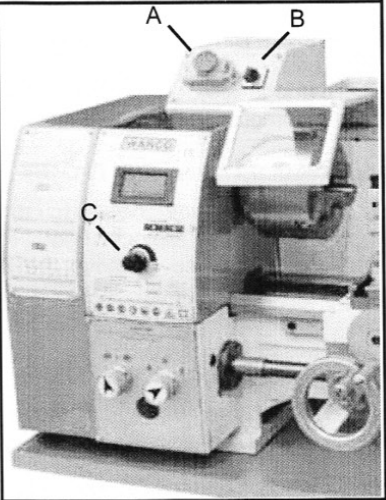
\includegraphics[width=3.1cm]{figure/asset/v4/paddle-image-0010-0001.png}};
\node[schema nota,text width=4.4cm] at (2.5,-6)
  {Asset originale};
\node[schema esterno,text width=7.7cm,minimum height=1.8cm] (padre) at (10.6,-1.45)
  {\textbf{Padre salvato in manual.json}\\\enquote{8. Cross Slide Lock}\\Associazione canonica non aggiornata};
\node[schema blocco,text width=7.7cm,minimum height=2.9cm] (contesto) at (10.6,-5)
  {\textbf{Contesto nella richiesta 0004}\\[4pt]
  A -- Emergency Button ON/OFF Switch\\
  B -- Change-over Switch\\
  C -- Variable Speed Control Switch\\[4pt]
  Sezioni che richiamano la Figura 11};
\draw[schema freccia,draw=schemaOcra] (5,-1.45) -- (padre.west);
\draw[schema freccia,draw=schemaBlu] (5,-5) -- (contesto.west);
\node[schema nota,text width=14.3cm] at (7.5,-7.45)
  {Il contesto della richiesta è più pertinente, ma il capitolo padre non viene corretto.};
\end{tikzpicture}
\caption{Due associazioni per \texttt{paddle-image-0010-0001}, da \texttt{manual.json} e dalla richiesta OCR \texttt{0004}. I richiami contestuali non sono nuovi capitoli. La discrepanza è ispezionabile anche se la caption viene esclusa per lunghezza.}
\label{fig:gerarchia-contesto-wm250}
\end{figure}

Anche le tavole delle pagine 26 e 33 rimangono sotto lo stesso capitolo, conseguenza della struttura parziale ottenuta senza l'indice. Nelle rispettive richieste capitolo e contesto locale sono però dichiarati non disponibili: il modello non riceve come argomento il titolo di una sezione lontana e non pertinente. La precauzione riduce un possibile condizionamento della descrizione, senza ricostruire la struttura mancante.

\subsection{Asset conservati ed effetti del filtro}

Tutte le 25 immagini dei due campioni conservano un riferimento a un asset presente nel bundle. Il confronto fra snapshot prima e dopo l'enrichment non evidenzia modifiche al testo acquisito, ai percorsi delle immagini o alla struttura dei capitoli: le differenze riguardano caption, provenance e campi di traccia associati alle esclusioni. Questa separazione permette di riesaminare l'estrazione senza confonderla con il contenuto generato.

Il filtro geometrico esclude sette immagini digitali e una scansionata. Sei delle sette esclusioni digitali appartengono alla pagina 98, dove il parser conserva sia la tastiera complessiva sia ritagli più piccoli; la settima è a pagina 352. Gli elementi esclusi non vengono eliminati. Il filtro evita così chiamate ripetute su frammenti di una stessa figura, ma non ricompone né deduplica la rappresentazione canonica.

Il caso scansionato rende evidente il costo della regola. Il ritaglio \texttt{paddle-image-0008-0003} occupa circa l'1,76\% della pagina e viene escluso perché inferiore al 2\%. Come mostra la Figura~\ref{fig:crop-escluso-wm250}, contiene tuttavia due manopole e simboli di comando riconoscibili: il filtro geometrico esclude quindi anche un asset con informazione tecnica. Non è stata generata una caption per questo asset e non è possibile attribuirgli un esito del VLM.

\begin{figure}[htbp]
\centering
\begin{tikzpicture}[schema base]
\node[schema titolo] at (0,0.3) {Dimensione del ritaglio e informazione visibile};
\node[schema etichetta] at (3.25,-0.6) {\textbf{Ingombro sulla pagina 8}};
\path[draw=schemaGrigio,fill=schemaGrigio!4] (0,-1.15) rectangle (6.5,-6.025);
\node[schema nota,text width=5.5cm] at (3.25,-2.15)
  {Pagina: $2600\times1950$\\Sistema di coordinate del bundle};
\path[draw=schemaOcra,fill=schemaCartaGialla,line width=1.2pt]
  ({1433/400},{-1.15-1052/400}) rectangle ({1761/400},{-1.15-1324/400});
\draw[schemaGrigio,line width=0.65pt]
  ({1433/400},-3.5) -- ({1761/400},-3.5);
\foreach \ascissa in {1433,1761} {
  \draw[schemaGrigio,line width=0.65pt] ({\ascissa/400},-3.42) -- ({\ascissa/400},-3.58);
}
\node[schema nota,font=\schemafont\footnotesize] at ({1597/400},-3.18) {328 px};
\draw[schemaGrigio,line width=0.65pt]
  (3.3,{-1.15-1052/400}) -- (3.3,{-1.15-1324/400});
\foreach \ordinata in {1052,1324} {
  \draw[schemaGrigio,line width=0.65pt] (3.22,{-1.15-\ordinata/400}) -- (3.38,{-1.15-\ordinata/400});
}
\node[schema nota,font=\schemafont\footnotesize,anchor=east] at (3.08,{-1.15-1188/400}) {272 px};
\node[schema nota,text width=5.7cm] at (3.25,-5.35)
  {Solo l'ingombro è rappresentato:\\non è il rendering della pagina.};
\node[schema etichetta] at (11.5,-0.6) {\textbf{Lo stesso ritaglio, ingrandito}};
\node[inner sep=0] (crop) at (11.5,-3.45)
  {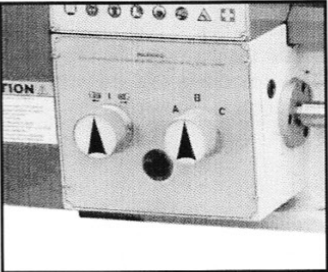
\includegraphics[width=4.6cm]{figure/asset/v4/paddle-image-0008-0003.png}};
\draw[schemaOcra,line width=1pt,line cap=round,line join=round]
  ([xshift=-3pt,yshift=-9pt]crop.north west) -- ([xshift=-3pt,yshift=3pt]crop.north west) -- ([xshift=9pt,yshift=3pt]crop.north west)
  ([xshift=-9pt,yshift=3pt]crop.north east) -- ([xshift=3pt,yshift=3pt]crop.north east) -- ([xshift=3pt,yshift=-9pt]crop.north east)
  ([xshift=-3pt,yshift=9pt]crop.south west) -- ([xshift=-3pt,yshift=-3pt]crop.south west) -- ([xshift=9pt,yshift=-3pt]crop.south west)
  ([xshift=-9pt,yshift=-3pt]crop.south east) -- ([xshift=3pt,yshift=-3pt]crop.south east) -- ([xshift=3pt,yshift=9pt]crop.south east);
\draw[schemaOcra,line width=1.1pt] (7.4,-2.65) circle (0.28);
\draw[schemaOcra,line width=1.8pt,line cap=round] (7.6,-2.85) -- (7.92,-3.17);
\draw[schema freccia,draw=schemaOcra] ({1761/400},{-1.15-1188/400}) -- (7.4,{-1.15-1188/400}) |- (crop.west);
\node[schema nota] at (11.5,-5.85) {Ritaglio: $328\times272$ pixel};
\node[schema blocco,text width=6.2cm,minimum height=1.9cm] at (3.5,-7.5)
  {\textbf{Regola geometrica}\\$\rho=\dfrac{328\cdot272}{2600\cdot1950}\simeq1{,}76\%$\\Inferiore alla soglia del $2\%$};
\node[schema esterno,text width=6.2cm,minimum height=1.9cm] at (11.5,-7.5)
  {\textbf{Conseguenza osservata}\\Nessuna chiamata al VLM\\Asset conservato, escluso dall'uso\\Comandi e simboli restano visibili};
\end{tikzpicture}
\caption{Filtro geometrico su \texttt{paddle-image-0008-0003}: a sinistra la posizione registrata in \texttt{manual.json}, a destra il ritaglio originale. L'immagine è esclusa prima della generazione, non per un errore del modello.}
\label{fig:crop-escluso-wm250}
\end{figure}

Il caso mostra il costo informativo della riduzione delle chiamate e l'utilità della conservazione degli scarti per valutarlo. L'effetto complessivo di un'eventuale eliminazione della soglia resta da verificare: la regola funziona come politica operativa, non come classificatore semantico validato.

\subsection{Tabelle: risultati storici e limite del campione finale}

Per lo schema 1.1 la matrice di accettazione riporta, in ciascuno dei due PDF digitali completi, 267 tabelle: 263 con serializzazione \texttt{structured}, quattro \texttt{unavailable} e nessuna in fallback, per 2341 righe serializzate. Le quattro indisponibilità corrispondono agli stessi elementi delle due varianti del manuale, per i quali Docling non aveva prodotto testo tabellare. Il ritaglio rimane disponibile, ma la serializzazione non ricostruisce celle assenti nell'estrazione.

Nel WM250 completo la matrice documenta dieci tabelle, nove strutturate e una indisponibile, per 289 righe. L'indisponibilità riguarda la pagina 32. Le selezioni digitali delle pagine 3 e 1004 documentano inoltre due tabelle strutturate e sei righe, inclusa la tabella degli allarmi EX1100--EX1104. Questi dati provengono dalle prove storiche, non dai due bundle V4.\footnote{\path{tesi-di-nardo/docs/acceptance-matrix.md}, sezione ``Chiusura dello schema 1.1'' e tabella dei run con prefisso \texttt{case1-schema11}, \texttt{case2-schema11} e \texttt{case3-schema11}.}

La distinzione fra output strutturato e testo indisponibile è un risultato utile della rappresentazione: il consumatore non riceve tutti i casi come se fossero tabelle complete. Non è invece dimostrata l'accuratezza di ogni cella o relazione intestazione--valore. Le caption tabellari riportate nelle vecchie selezioni appartengono al setup storico; nel workflow finale le tabelle sono serializzate senza essere inviate al VLM. Poiché le selezioni V4 contengono zero elementi \texttt{table}, non forniscono una nuova misura empirica di qualità tabellare.

\section{Esiti dell'arricchimento multimodale}
\label{sec:risultati-enrichment}

\subsection{Bilancio delle richieste e delle caption}

Le 17 chiamate finali si distribuiscono in otto esiti \texttt{enriched}, cinque \texttt{review\_required} e quattro \texttt{failed}. Le otto immagini saltate prima della chiamata non appartengono a questo denominatore. La Tabella~\ref{tab:esiti-caption} conserva la distinzione tra filtraggio, generazione e ammissibilità finale.

\begin{table}[!htbp]
\centering
\caption{Bilancio V4 da \texttt{diagnostics/enrichment.json} e \texttt{manual.json}. I gruppi descrivono stadi diversi e non vanno sommati tra loro. Tutti i 25 asset restano conservati; l'ammissibilità non misura l'accuratezza semantica.}
\label{tab:esiti-caption}
\small
\begin{tabularx}{\textwidth}{@{}Xrrr@{}}
\toprule
Fase e conteggio & Digitale & Scansione & Totale \tabularnewline
\midrule
\multicolumn{4}{@{}l}{\textbf{Acquisizione e filtro: 25 immagini}} \tabularnewline
Immagini acquisite & 16 & 9 & 25 \\
Escluse dal filtro prima della chiamata & 7 & 1 & 8 \tabularnewline
Richieste al provider & 9 & 8 & 17 \\
\midrule
\multicolumn{4}{@{}l}{\textbf{Generazione: 17 richieste, tre esiti disgiunti}} \tabularnewline
\texttt{enriched}: ammissibile secondo la politica & 7 & 1 & 8 \tabularnewline
\texttt{review\_required}: da rivedere & 1 & 4 & 5 \tabularnewline
\texttt{failed}: risposta fuori contratto & 1 & 3 & 4 \tabularnewline
\midrule
\multicolumn{4}{@{}l}{\textbf{Conservazione nel documento finale}} \tabularnewline
Caption presenti (ammissibili + da rivedere) & 8 & 5 & 13 \tabularnewline
Di cui con inclusione prevista attiva & 7 & 1 & 8 \tabularnewline
\bottomrule
\end{tabularx}
\end{table}

Il rapporto otto su diciassette descrive le richieste che producono una caption ammissibile secondo la politica implementata. Non è una misura di accuratezza. Delle tredici caption presenti, cinque sono conservate per la revisione ma escluse dall'inclusione prevista; le altre otto sono ammissibili per l'uso successivo secondo la politica.

\subsection{Aggiunte supportate e informazioni già disponibili}

Nell'immagine digitale di pagina 73, \texttt{docling-image-0073-0001}, la caption nomina le fasi U, V e W con le sigle L1, L2 e L3, il riferimento QF1 e la terra di protezione PE. Queste etichette sono visibili nel ritaglio. L'output converte quindi dettagli grafici in testo esplicito, pur essendo marcato per revisione a causa della natura elettrica del contenuto.

Il guadagno informativo non coincide con l'intera descrizione: il testo di contesto già menziona cavo, interruttore QF1 e avvertenza di spegnimento. La presenza di tali informazioni nella caption non è una scoperta visuale. Il contributo osservabile è più circoscritto e riguarda la trascrizione e l'organizzazione di etichette che il contesto fornito non enumerava nello stesso modo. Il caso mostra che una descrizione esclusa per ragioni prudenziali può contenere informazioni supportate; lo stato tecnico non è un giudizio globale sul suo contenuto.

Nella seconda immagine OCR di pagina 10, \texttt{paddle-image-0010-0002}, la caption identifica i selettori D ed E e collega la figura all'avanzamento del carrello. Tuttavia, il prompt contiene già i paragrafi \enquote{Feed Direction Selector} e \enquote{Feed Rate Selector}. Parte della descrizione riformula pertanto la baseline testuale. Il confronto non consente di attribuire al solo canale visuale la comprensione della funzione dei comandi, né dimostra un miglioramento del loro recupero mediante ricerca.

\subsection{Errori presenti anche nelle caption accettate}

Un controesempio diretto alla coincidenza fra formato e correttezza è fornito dall'immagine \texttt{docling-image-0225-0010}. La risposta descrive una barra con \enquote{10 pulsanti quadrati neri}; nel ritaglio sono visibili dodici pulsanti. La stessa risposta coglie correttamente l'evidenziazione del primo mediante un cerchio rosa, ma il conteggio è errato. La caption, lunga 486 caratteri, riceve \texttt{enriched} e l'immagine mantiene l'inclusione prevista attiva.

La Figura~\ref{fig:errore-caption-menu} permette di confrontare il conteggio visibile con l'affermazione generata e con lo stato assegnato.

\begin{figure}[htbp]
\centering
\begin{tikzpicture}[schema base]
\node[schema titolo] at (0,0.3) {Conteggio visibile e conteggio generato};
\node[schema nota,anchor=west] at (0,-0.35) {Asset digitale originale -- pagina 225, chiamata 0004};
\node[anchor=north west,inner sep=0] at (0.3,-0.9)
  {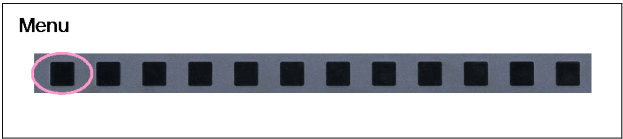
\includegraphics[width=14.4cm]{figure/asset/v4/docling-image-0225-0010.png}};
\foreach \numero/\pixel in {1/62,2/108,3/154,4/200,5/246,6/292,7/338,8/384,9/430,10/476,11/522,12/568} {
  \draw[schema icona,draw=schemaBlu!70,line width=0.5pt]
    ({0.3+14.4*\pixel/623},-4.6) -- ({0.3+14.4*\pixel/623},{-0.9-14.4*92/623});
  \node[font=\schemafont\footnotesize,text=schemaBlu] at ({0.3+14.4*\pixel/623},-4.95) {\numero};
}
\node[schema nota,text width=14cm] at (7.5,-5.55)
  {Numerazione editoriale aggiunta per rendere controllabile il conteggio: 12 pulsanti.};
\node[schema blocco,text width=6.2cm,minimum height=2cm] at (3.5,-7.35)
  {\textbf{Che cosa afferma la caption}\\[4pt]
  \enquote{10 pulsanti quadrati neri}\\[4pt]
  Il primo è descritto correttamente\\come cerchiato in rosa.};
\node[schema esterno,text width=6.2cm,minimum height=2cm] at (11.5,-7.35)
  {\textbf{Che cosa attestano i controlli}\\[4pt]
  Stato: \texttt{enriched}\\Inclusione prevista: attiva\\Formato accettato, conteggio non verificato};
\end{tikzpicture}
\caption{La caption di \texttt{docling-image-0225-0010} conta dieci pulsanti, ma nell'immagine sono dodici: il controllo di formato non rileva l'errore. Numeri e linee sono aggiunti per il confronto; il cerchio rosa è nell'originale.}
\label{fig:errore-caption-menu}
\end{figure}

La descrizione della schermata digitale di pagina 228, \texttt{docling-image-0228-0013}, introduce invece l'espressione \enquote{posizionamento robotico}. La fonte contestuale riguarda le coordinate e i punti utente della macchina ROBOCUT e non giustifica tale qualificazione. La risposta viene esclusa per lunghezza, non perché il controllo abbia riconosciuto l'interpretazione non supportata. Il motivo tecnico del fallimento e il problema semantico osservato devono quindi essere annotati separatamente.

Questi esempi non permettono di stimare il tasso di errore dell'intero campione. Consentono però di escludere una conclusione più forte ma ingiustificata: nessuno degli stati automatici garantisce che tutti i dettagli della caption siano fedeli. Un testo formalmente corretto può includere errori insieme a osservazioni esatte.

\subsection{Omissioni e comportamento dei controlli di revisione}

Per la tavola esplosa OCR di pagina 26, \texttt{paddle-image-0026-0001}, la risposta si concentra su categorie generiche quali ingranaggi, cuscinetti e trasmissione. Non riproduce le associazioni fra i numerosi riferimenti numerati e le parti; una descrizione così sintetica non sostituisce la tavola quando occorre identificare un componente specifico. Il limite di otto elementi nel prompt è compatibile con questa compressione, ma una sola esecuzione non consente di attribuirgli causalmente tutte le omissioni.

La caption classifica l'immagine come \enquote{schema/diagramma} e menziona un \enquote{motore elettrico}. La diagnostica richiede revisione per schema elettrico. Il comportamento è coerente con la regola lessicale implementata, che cerca termini elettrici nei campi descrittivi di un diagramma; non dimostra però che la tavola sia uno schema di cablaggio. L'asset è una rappresentazione esplosa di un gruppo meccanico. Il caso mostra come un controllo prudenziale possa intercettare un'espressione della risposta senza classificare semanticamente il documento sorgente.

Gli altri tre casi OCR da rivedere sono \texttt{paddle-image-0008-0004}, \texttt{paddle-image-0010-0003} e \texttt{paddle-image-0033-0001}. Il motivo salvato è una contraddizione tra la dichiarazione di assenza di incertezze e una lettura indicata come non possibile. Il controllo opera su formulazioni linguistiche: non verifica autonomamente se il dettaglio sia illeggibile, assente o semplicemente non pertinente. La segnalazione è quindi un invito alla revisione e può essere conservativa; non equivale a una valutazione umana già svolta.

Nel complesso, il ciclo V4 evidenzia aggiunte supportate, ripetizioni della baseline, omissioni e interpretazioni errate. Non fornisce una misura di beneficio netto dell'enrichment. Tale conclusione non nega che alcune caption siano informative: distingue l'esistenza di contributi utili dalla dimostrazione di un miglioramento complessivo e trasferibile.

\section{Esiti dei controlli, fallimenti e tracciabilità}
\label{sec:errori}

\subsection{Fallimenti delle caption senza perdita del bundle}

Tutti i quattro esiti \texttt{failed} delle richieste V4 sono associati al superamento del limite di 1200 caratteri. Le risposte restano conservate nelle evidenze del provider, ma non vengono pubblicate come caption generate nel documento. Le lunghezze riguardano il testo normalizzato, non i token o i byte HTTP. Le chiamate escluse sono D07 (1207 caratteri; eccedenza 7), S01 (1370; eccedenza 170), S02 (1360; eccedenza 160) e S04 (1210; eccedenza 10): le sigle identificano le registrazioni digitali e OCR usate nel grafico.

La Figura~\ref{fig:lunghezze-caption-v4} colloca le quattro esclusioni rispetto alle altre tredici risposte e alla soglia del contratto. Include anche le risposte non pubblicate come caption, evitando di rappresentare soltanto gli esiti conservati nel documento.

\begin{figure}[!htbp]
\centering
\begin{tikzpicture}[schema base,schema nota/.append style={font=\schemafont\footnotesize}]
\node[schema titolo] at (0,0.7) {Lunghezza delle risposte e stato assegnato};
\foreach \valore in {0,300,600,900,1200,1500} {
  \draw[draw=schemaGrigio!20,line width=0.4pt] ({3.4+0.007*\valore},-0.9) -- ({3.4+0.007*\valore},-10.65);
  \node[schema nota] at ({3.4+0.007*\valore},-11) {\valore};
}
\draw[draw=schemaOcra,dash pattern=on 4pt off 3pt,line width=1pt] (11.8,-0.65) -- (11.8,-10.65);
\node[schema nota,text=schemaOcra] at (11.8,0) {Limite: 1200};
\node[schema titolo] at (0,-1) {Digitale: 9 risposte};
\node[schema titolo] at (0,-6) {Scansione: 8 risposte};
\node[schema etichetta,anchor=east] at (3.1,-1.800) {D01 -- p. 73};
\draw[draw=schemaOcra!45,line width=0.8pt] (3.4,-1.800) -- (8.2510,-1.800);
\path[draw=schemaOcra,fill=schemaOcra!25] (8.1760,-1.875) rectangle +(0.15,0.15);
\node[schema nota,anchor=west] at (8.3810,-1.800) {693};
\node[schema etichetta,anchor=east] at (3.1,-2.260) {D02 -- p. 93};
\draw[draw=schemaVerde!45,line width=0.8pt] (3.4,-2.260) -- (9.9310,-2.260);
\fill[schemaVerde] (9.9310,-2.260) circle (0.075);
\node[schema nota,anchor=west] at (10.0610,-2.260) {933};
\node[schema etichetta,anchor=east] at (3.1,-2.720) {D03 -- p. 98};
\draw[draw=schemaVerde!45,line width=0.8pt] (3.4,-2.720) -- (8.6220,-2.720);
\fill[schemaVerde] (8.6220,-2.720) circle (0.075);
\node[schema nota,anchor=west] at (8.7520,-2.720) {746};
\node[schema etichetta,anchor=east] at (3.1,-3.180) {D04* -- p. 225};
\draw[draw=schemaVerde!45,line width=0.8pt] (3.4,-3.180) -- (6.8020,-3.180);
\fill[schemaVerde] (6.8020,-3.180) circle (0.075);
\node[schema nota,anchor=west] at (6.9320,-3.180) {486};
\node[schema etichetta,anchor=east] at (3.1,-3.640) {D05 -- p. 225};
\draw[draw=schemaVerde!45,line width=0.8pt] (3.4,-3.640) -- (9.8960,-3.640);
\fill[schemaVerde] (9.8960,-3.640) circle (0.075);
\node[schema nota,anchor=west] at (10.0260,-3.640) {928};
\node[schema etichetta,anchor=east] at (3.1,-4.100) {D06 -- p. 228};
\draw[draw=schemaVerde!45,line width=0.8pt] (3.4,-4.100) -- (8.7690,-4.100);
\fill[schemaVerde] (8.7690,-4.100) circle (0.075);
\node[schema nota,anchor=west] at (8.8990,-4.100) {767};
\node[schema etichetta,anchor=east] at (3.1,-4.560) {D07 -- p. 228};
\draw[draw=schemaGrigio!45,line width=0.8pt] (3.4,-4.560) -- (11.8490,-4.560);
\draw[draw=schemaGrigio,line width=1.2pt] (11.7740,-4.635) -- ++(0.15,0.15) (11.7740,-4.485) -- ++(0.15,-0.15);
\node[schema nota,anchor=west] at (11.9790,-4.560) {1207};
\node[schema etichetta,anchor=east] at (3.1,-5.020) {D08 -- p. 352};
\draw[draw=schemaVerde!45,line width=0.8pt] (3.4,-5.020) -- (9.8890,-5.020);
\fill[schemaVerde] (9.8890,-5.020) circle (0.075);
\node[schema nota,anchor=west] at (10.0190,-5.020) {927};
\node[schema etichetta,anchor=east] at (3.1,-5.480) {D09 -- p. 352};
\draw[draw=schemaVerde!45,line width=0.8pt] (3.4,-5.480) -- (10.2040,-5.480);
\fill[schemaVerde] (10.2040,-5.480) circle (0.075);
\node[schema nota,anchor=west] at (10.3340,-5.480) {972};
\node[schema etichetta,anchor=east] at (3.1,-6.800) {S01 -- p. 8};
\draw[draw=schemaGrigio!45,line width=0.8pt] (3.4,-6.800) -- (12.9900,-6.800);
\draw[draw=schemaGrigio,line width=1.2pt] (12.9150,-6.875) -- ++(0.15,0.15) (12.9150,-6.725) -- ++(0.15,-0.15);
\node[schema nota,anchor=west] at (13.1200,-6.800) {1370};
\node[schema etichetta,anchor=east] at (3.1,-7.260) {S02 -- p. 8};
\draw[draw=schemaGrigio!45,line width=0.8pt] (3.4,-7.260) -- (12.9200,-7.260);
\draw[draw=schemaGrigio,line width=1.2pt] (12.8450,-7.335) -- ++(0.15,0.15) (12.8450,-7.185) -- ++(0.15,-0.15);
\node[schema nota,anchor=west] at (13.0500,-7.260) {1360};
\node[schema etichetta,anchor=east] at (3.1,-7.720) {S03 -- p. 8};
\draw[draw=schemaOcra!45,line width=0.8pt] (3.4,-7.720) -- (10.4210,-7.720);
\path[draw=schemaOcra,fill=schemaOcra!25] (10.3460,-7.795) rectangle +(0.15,0.15);
\node[schema nota,anchor=west] at (10.5510,-7.720) {1003};
\node[schema etichetta,anchor=east] at (3.1,-8.180) {S04 -- p. 10};
\draw[draw=schemaGrigio!45,line width=0.8pt] (3.4,-8.180) -- (11.8700,-8.180);
\draw[draw=schemaGrigio,line width=1.2pt] (11.7950,-8.255) -- ++(0.15,0.15) (11.7950,-8.105) -- ++(0.15,-0.15);
\node[schema nota,anchor=west] at (12.0000,-8.180) {1210};
\node[schema etichetta,anchor=east] at (3.1,-8.640) {S05 -- p. 10};
\draw[draw=schemaVerde!45,line width=0.8pt] (3.4,-8.640) -- (8.4120,-8.640);
\fill[schemaVerde] (8.4120,-8.640) circle (0.075);
\node[schema nota,anchor=west] at (8.5420,-8.640) {716};
\node[schema etichetta,anchor=east] at (3.1,-9.100) {S06 -- p. 10};
\draw[draw=schemaOcra!45,line width=0.8pt] (3.4,-9.100) -- (11.0790,-9.100);
\path[draw=schemaOcra,fill=schemaOcra!25] (11.0040,-9.175) rectangle +(0.15,0.15);
\node[schema nota,anchor=east,fill=white,inner sep=1.5pt] at (10.9490,-9.100) {1097};
\node[schema etichetta,anchor=east] at (3.1,-9.560) {S07 -- p. 26};
\draw[draw=schemaOcra!45,line width=0.8pt] (3.4,-9.560) -- (7.5860,-9.560);
\path[draw=schemaOcra,fill=schemaOcra!25] (7.5110,-9.635) rectangle +(0.15,0.15);
\node[schema nota,anchor=west] at (7.7160,-9.560) {598};
\node[schema etichetta,anchor=east] at (3.1,-10.020) {S08 -- p. 33};
\draw[draw=schemaOcra!45,line width=0.8pt] (3.4,-10.020) -- (8.5170,-10.020);
\path[draw=schemaOcra,fill=schemaOcra!25] (8.4420,-10.095) rectangle +(0.15,0.15);
\node[schema nota,anchor=west] at (8.6470,-10.020) {731};
\draw[draw=schemaGrigio,line width=0.7pt] (3.4,-10.65) -- (13.9,-10.65);
\node[schema etichetta] at (8.65,-11.65) {Caratteri del testo normalizzato, non token};
\fill[schemaVerde] (0.6,-12.5) circle (0.075);
\node[schema nota,anchor=west] at (0.85,-12.5) {\texttt{enriched}};
\path[draw=schemaOcra,fill=schemaOcra!25] (5,-12.575) rectangle +(0.15,0.15);
\node[schema nota,anchor=west] at (5.3,-12.5) {\texttt{review\_required}};
\draw[draw=schemaGrigio,line width=1.2pt] (11,-12.575) -- ++(0.15,0.15) (11,-12.425) -- ++(0.15,-0.15);
\node[schema nota,anchor=west] at (11.3,-12.5) {\texttt{failed}};
\node[schema nota,text width=14.4cm] at (7.5,-13.55)
  {D/S: digitale/scansione; numero della chiamata; p.: pagina fisica del PDF.\\
  * D04 contiene il conteggio errato dei pulsanti, pur essendo sotto soglia.};
\end{tikzpicture}
\caption{Lunghezza delle 17 risposte V4, dai \protect\path{caption-response.json}, incluse le quattro escluse per lunghezza. Le otto immagini filtrate prima della generazione non compaiono. Il caso D04 è illustrato nella Figura~\ref{fig:errore-caption-menu}.}
\label{fig:lunghezze-caption-v4}
\end{figure}

Le eccedenze di sette e dieci caratteri rendono evidente la natura rigida del contratto: l'esclusione non è proporzionale alla qualità del contenuto. Non ne consegue che sia corretto troncare automaticamente le risposte o aumentare la soglia sulla base di questi soli esempi. Entrambe le modifiche cambierebbero il trattamento dell'output e richiederebbero nuove verifiche, in particolare per non perdere il campo delle incertezze.

Diversamente dall'esito V3 descritto nel diario, nel quale le caption fuori contratto avevano impedito la pubblicazione, le due run V4 mantengono gli altri risultati e pubblicano bundle sperimentali. La documentazione V3 è evidenza storica, non un'esecuzione qui ripetuta; la continuità V4 è invece osservabile negli artefatti. Il miglioramento sostenuto dai dati riguarda la gestione del fallimento locale, non un aumento dimostrato dell'accuratezza delle descrizioni.

\FloatBarrier
\subsection{Validazione e gate di promozione}

I report salvati superano tutti i 30 controlli dello schema 1.1. Le ragioni che impediscono lo stato \texttt{validated} sono leggibili separatamente nella diagnostica di promozione, riportata nella Tabella~\ref{tab:gate-v4}.

\begin{table}[!htbp]
\centering
\caption{Gate di promozione da \texttt{diagnostics/promotion.json}. ``No'' indica un requisito non soddisfatto, non necessariamente incoerenza tecnica. Il requisito sull'enrichment considera anche gli errori delle singole richieste.}
\label{tab:gate-v4}
\small
\begin{tabularx}{\textwidth}{@{}Xcc@{}}
\toprule
Requisito di promozione & Digitale & Scansione \tabularnewline
\midrule
Documento elaborato integralmente\newline{\footnotesize\texttt{document.full}} & No & No \tabularnewline
Enrichment configurato e senza errori\newline{\footnotesize\texttt{enrichment.configured}} & No & No \tabularnewline
Identità delle caption coerente\newline{\footnotesize\texttt{captions.identity}} & Sì & Sì \tabularnewline
Nessuna caption da rivedere\newline{\footnotesize\texttt{enrichment.review\_free}} & No & No \tabularnewline
Nessun avviso ostativo\newline{\footnotesize\texttt{warnings.nonconsequential}} & Sì & No \tabularnewline
Profilo accettato\newline{\footnotesize\texttt{profile.accepted}} & Sì & Sì \tabularnewline
Strategia strutturale accettata\newline{\footnotesize\texttt{structure.accepted}} & Sì & No \tabularnewline
\bottomrule
\end{tabularx}
\end{table}

Per entrambi i casi pesano la selezione parziale, i fallimenti del captioning e gli elementi da rivedere. Nel digitale gli avvisi su due corrispondenze normalizzate dei titoli non impediscono il superamento del gate sugli avvisi. Nel caso scansionato incidono anche i limiti della struttura parziale e il fallback. Il profilo OCR risulta accettato tramite l'evidenza storica registrata, ma questa accettazione non basta a promuovere una run che ne utilizza un percorso strutturale meno affidabile.

La combinazione fra report passato e stato sperimentale non è contraddittoria. Il report conferma che lo stato e gli artefatti rispettano il contratto e la politica; non afferma che tutti i gate di promozione siano superati. L'errore di conteggio della Figura~\ref{fig:errore-caption-menu} mostra inoltre che neppure il superamento dei controlli della singola caption coincide con la correttezza semantica.

\subsection{Integrità degli artefatti e identificazione della revisione}

L'audit descritto nella Sezione~\ref{sec:audit-metodi} conferma la corrispondenza delle fingerprint dei due bundle con i valori salvati. I digest iniziano rispettivamente con \texttt{395963bbb6ba} e \texttt{b8827d3573df}; i valori completi rimangono nei report. Risultano coerenti anche gli hash degli asset inviati, i prompt salvati e le risposte HTTP rispetto al testo normalizzato conservato nelle evidenze. Le tredici caption presenti nel documento hanno un hash di ingresso ricostruibile dagli asset e dalle richieste.

Questa catena rende controllabili anche gli esiti esclusi: è possibile distinguere un asset mai inviato, una risposta generata ma fuori contratto e una caption conservata soltanto per revisione. I contatori del report possono essere confrontati con le chiamate individuali. L'uguaglianza fra snapshot dopo l'enrichment e documento finale, in questi campioni privi di tabelle, conferma inoltre che il contenuto generativo valutato è quello effettivamente pubblicato.

Resta una limitazione dell'identità software: 32 dei 34 sorgenti registrati per ciascuna run corrispondono ai file conservati nell'archivio del progetto, mentre \texttt{enrichment.py} e \texttt{orchestrator.py} hanno hash diversi. Mancano anche lo script di strumentazione e alcuni materiali del protocollo. L'audit conferma dunque l'integrità dei bundle rispetto alle loro impronte; per la riproduzione esatta delle run occorre invece recuperare la revisione eseguita e i materiali mancanti. La verifica si limita agli artefatti conservati, senza rieseguire la suite di test o la validazione completa del corpus.

\section{Discussione, limiti e trasferibilità}
\label{sec:limiti}

\subsection{Contributo dell'integrazione}

Il risultato principale è l'organizzazione di percorsi eterogenei in un workflow con contratto comune e stati espliciti. Le prove complete documentate e i bundle selettivi mostrano che struttura, testo, asset, descrizioni e tracce possono essere rappresentati senza imporre ai consumatori il formato nativo di ciascun parser. Il valore dell'integrazione risiede anche nel rendere visibili i limiti degli stadi: una tabella può essere indisponibile, una caption può fallire e una run può restare sperimentale senza essere confusa con un output corrotto.

La convergenza formale non risolve ogni problema documentale. Il caso OCR di pagina 10 dimostra che un riferimento padre valido può essere semanticamente inadeguato. La selezione di un contesto migliore per il prompt è una mitigazione locale, non una correzione dell'intero modello gerarchico. La qualità va quindi verificata anche nelle relazioni, non soltanto nella presenza degli elementi.

\subsection{Compromessi dell'enrichment e dei controlli}

Gli esempi non sostengono né l'accettazione indiscriminata delle descrizioni né il loro rifiuto complessivo. Nel medesimo ciclo si osservano trascrizioni visuali supportate, informazioni già presenti nel contesto, conteggi errati e descrizioni troppo generiche. I controlli intercettano vincoli di formato e segnali linguistici, ma possono lasciare passare errori semantici o inviare a revisione casi che richiedono un'interpretazione più fine della fonte.

Anche le esclusioni hanno un costo. Il ritaglio WM250 sotto soglia contiene comandi riconoscibili; alcune risposte vengono scartate per un'eccedenza minima di lunghezza; le descrizioni elettriche restano escluse pur potendo contenere etichette corrette. La trasparenza di questi esiti consente di valutare il compromesso scelto fra copertura e prudenza, la cui ottimalità resta da verificare.

La separazione finale fra immagini al VLM e tabelle serializzate riduce le occasioni di riscrittura generativa dei dati tabellari. Non rende però automaticamente corrette le celle acquisite. La fedeltà del parser e quella della trasformazione successiva restano due problemi distinti, da valutare con riferimenti appropriati.

\subsection{Validità e generalizzazione}

Il corpus comprende due manuali di base e tre condizioni di ingresso; le due varianti digitali non sono indipendenti. La selezione di 17 immagini deriva dal percorso di sviluppo della pipeline, non da un campione esterno o casuale. Lo studio non comprende repliche delle generazioni o un'annotazione indipendente completa; inoltre, i PDF integrali sono assenti dall'archivio del progetto. Questi limiti impediscono di stimare generalizzazione, variabilità o tassi semantici globali con un significato statistico fondato.

Il confronto tra digitale e scansione è inoltre confuso da differenze di documento, lingua, layout e struttura disponibile. Il maggiore numero di esclusioni successive alla generazione nel caso OCR non isola l'effetto del parser o della qualità dell'immagine. Analogamente, le metriche storiche della TOC e i conteggi delle tabelle non sostituiscono l'analisi diretta delle corrispondenze o delle celle.

Infine, non sono stati misurati retrieval, qualità delle risposte dell'assistente o prestazioni degli operatori dopo l'introduzione di questa pipeline. La presenza di testo visuale aggiuntivo è una condizione che può essere sfruttata a valle, non una prova di efficacia. Le conclusioni sostenute dal lavoro riguardano l'integrazione dell'ingestion, l'ispezionabilità degli esiti e i limiti emersi nella rappresentazione e nell'enrichment.
\chapter{Conclusioni}
\label{cap:conclusioni}

\section{Sintesi del contributo}

La tesi affronta la preparazione dei manuali tecnici prima del retrieval, distinguendo tale problema dalla costruzione dell'assistente industriale completo. Il contributo è una pipeline integrata che seleziona automaticamente una strategia di acquisizione, organizza i contenuti in una rappresentazione gerarchica comune e conserva elementi, asset e provenienza in un bundle verificabile. La CLI ne costituisce l'interfaccia operativa; i contratti, la diagnostica e la pubblicazione atomica ne rendono espliciti gli esiti.

Le evidenze combinano prove storiche documentate per tre profili e due esecuzioni selettive finali direttamente ispezionabili. I tre file di ingresso corrispondono a due manuali di base: una coppia digitale con e senza outline e un manuale scansionato distinto. Il ciclo V4 mostra l'elaborazione di 17 immagini mediante il modello locale, mantenendo separata la serializzazione deterministica delle tabelle. I bundle vengono pubblicati come sperimentali e conservano sia i risultati utilizzabili secondo la politica sia le motivazioni delle esclusioni.

La valutazione ha messo in luce limiti semantici anche in una rappresentazione formalmente coerente: un'associazione gerarchica OCR non pertinente, una caption accettata con un conteggio errato e un ritaglio informativo escluso per dimensione. Allo stesso tempo, la separazione fra fonte, descrizione e decisione rende questi limiti ricostruibili. Il contributo sostenuto dalle evidenze è quindi l'integrazione di una preparazione documentale ispezionabile, non una garanzia di accuratezza automatica né un miglioramento dimostrato del sistema RAG downstream.

\section{Risposte alle domande di ricerca}

\subsection{RQ1 --- Ingestion integrata}

\emph{Come ricondurre manuali PDF eterogenei, attraverso strategie di acquisizione differenti, a una rappresentazione gerarchica comune, e quali limiti emergono nella conservazione dei contenuti e dei loro collegamenti?}

La soluzione sviluppata separa il recupero dei contenuti e della struttura dalle trasformazioni condivise. L'outline incorporato, la ricostruzione dall'indice stampato e l'acquisizione OCR alimentano lo stesso assemblatore e lo stesso contratto \texttt{ManualDocument}. Le prove storiche riportate nella Sezione~\ref{sec:risultati-struttura} documentano la copertura dei tre profili, mentre i bundle V4 rendono direttamente osservabile la convergenza di due percorsi su artefatti omogenei.

Il limite principale emerso è la differenza fra coerenza delle relazioni e correttezza della loro interpretazione. Nella selezione OCR più figure rimangono associate all'ultima sezione della pagina, anche quando il contesto della richiesta viene ricondotto alla figura corretta. La conservazione degli asset permette di verificarlo, ma non lo risolve. La risposta a RQ1 è pertanto positiva quanto alla realizzazione del contratto comune e circoscritta quanto alla fedeltà: non è dimostrata la conservazione completa di ogni contenuto o relazione su famiglie di manuali diverse da quelle studiate.

\subsection{RQ2 --- Arricchimento}

\emph{Quali informazioni aggiuntive, omissioni ed errori introduce l'arricchimento multimodale locale rispetto ai contenuti già disponibili dall'estrazione?}

Il captioning può rendere esplicite etichette visuali, disposizioni e riferimenti altrimenti confinati nel ritaglio. L'esempio delle fasi e della terra di protezione mostra aggiunte supportate, mentre altri passaggi delle descrizioni ripetono informazioni già presenti nel contesto. Nel ciclo finale coesistono inoltre errori di conteggio, qualificazioni non supportate e sintesi che non preservano tutte le relazioni delle tavole tecniche, come documentato nella Sezione~\ref{sec:risultati-enrichment}.

Otto delle 17 richieste ricevono lo stato \texttt{enriched}, cinque richiedono revisione e quattro falliscono il contratto di lunghezza. Questi sono esiti tecnici, non punteggi di accuratezza: la caption che indica dieci pulsanti anziché dodici rientra fra quelle accettate. Per le tabelle il workflow finale evita la generazione e conserva una serializzazione delle informazioni acquisite; i due campioni V4 non ne misurano nuovamente la qualità.

Non è quindi dimostrato un beneficio netto dell'enrichment. È invece documentata la necessità di distinguere aggiunte reali, riformulazioni della baseline, omissioni ed errori, includendo nella valutazione le risposte escluse. Una maggiore quantità di testo non può essere assunta come miglioramento della rappresentazione o della consultazione del manuale.

\subsection{RQ3 --- Verificabilità}

\emph{In che modo provenienza e controlli consentono di verificare gli esiti della pipeline e di distinguerne la conformità tecnica dalla correttezza semantica?}

Manifest, hash degli ingressi, snapshot, registrazioni delle richieste e diagnostica consentono di ricostruire quale asset è stato elaborato, con quale contesto, quale risposta è stata prodotta e perché essa sia stata inclusa, esclusa o destinata a revisione. La Sezione~\ref{sec:errori} mostra che un report con controlli superati può accompagnare correttamente un bundle sperimentale: la conformità riguarda anche la dichiarazione veritiera dei limiti, non soltanto il successo del percorso ordinario.

La verifica delle fingerprint e delle richieste sostiene l'integrità dei materiali conservati. Il confronto con il contenuto visuale resta però necessario per accertare le affermazioni delle caption e la pertinenza dei collegamenti documentali. Inoltre, la mancata corrispondenza di due sorgenti agli hash registrati e l'assenza di parte dei materiali limitano la riproduzione esatta. La risposta a RQ3 è dunque che la provenienza rende gli esiti controllabili e le anomalie localizzabili, ma non sostituisce né la verifica semantica né la disponibilità completa dell'ambiente sperimentale.

\section{Sviluppi futuri}

\subsection{Consolidamento della pipeline documentale}

La prima priorità è completare il pacchetto di riproducibilità: PDF identificati dagli hash, revisione esatta dei sorgenti, script di strumentazione, protocollo e schede qualitative. La conservazione delle dipendenze e delle caratteristiche del runtime dovrebbe permettere di ripetere le esecuzioni nelle condizioni documentate, andando oltre la verifica d'integrità dei bundle conservati. Questa attività precede l'estensione del corpus, perché rende confrontabili le prove successive.

Sul piano strutturale, il caso OCR suggerisce di collegare le figure alle sezioni che le richiamano anche nel documento canonico, non soltanto nel prompt. La correzione dovrebbe gestire riferimenti multipli e ambigui senza imporre sempre un unico padre semantico. È inoltre necessario verificare esplicitamente i documenti parziali e i confini fra sezioni sulla stessa pagina, evitando che un titolo locale venga esteso a tavole successive prive di intestazione.

Per gli asset e l'enrichment, le priorità derivano dai fallimenti osservati: riesaminare il filtro geometrico su figure piccole ma informative; distinguere meglio testo assente e testo illeggibile; verificare numeri e sigle contro la fonte; valutare controlli di revisione meno dipendenti da sole parole chiave. Le soglie di lunghezza e il limite di otto elementi richiedono una valutazione su materiali separati da quelli usati per modificarli. Allungare il prompt o ammettere tutte le caption non costituirebbe, di per sé, una soluzione ai problemi semantici.

La verifica dovrebbe estendersi a nuovi manuali, con criteri di annotazione espliciti, revisione indipendente e conservazione dei disaccordi. Repliche delle generazioni permetterebbero di distinguere errori ricorrenti e variabilità delle singole risposte. Per le tabelle occorre affiancare ai test della serializzazione il confronto tra celle, intestazioni e fonte, separando gli errori del parser da quelli introdotti dalle trasformazioni successive.

\subsection{Integrazione e valutazione downstream}

L'integrazione con il sistema RAG del progetto quadro costituisce una fase distinta. Un confronto controllato dovrebbe mantenere uguali corpus, chunking, modello di embedding e procedura di retrieval, variando il contributo delle caption o della rappresentazione tabellare. Le domande di prova dovrebbero includere richieste per cui figura, posizione di un comando o relazione fra celle siano effettivamente necessarie, senza limitarsi a quesiti già risolvibili dal testo circostante.

Solo dopo aver verificato il recupero e le risposte dell'assistente sarebbe possibile valutare l'effetto sull'attività degli operatori. Uno studio human-in-the-loop richiederebbe un protocollo specifico, compiti comparabili e misure di prestazione ed esperienza d'uso; non sarebbe sostituibile con i conteggi dei bundle o delle caption. Le misure del progetto quadro richiamate nell'Introduzione non sono risultati della pipeline qui studiata.

La Figura~\ref{fig:confronto-rag-futuro} traduce questa direzione in uno schema di confronto: la variazione documentale viene isolata prima di estendere la valutazione al lavoro degli operatori.

\begin{figure}[!htbp]
\centering
\begin{tikzpicture}[schema base]
\node[schema esterno,text width=13.7cm] at (7.5,0)
  {\textbf{Proposta di confronto: non eseguita nella tesi}\\Stessi corpus, domande, chunking, embedding, retrieval e generatore};
\node[schema etichetta] at (3.3,-1.35) {\textbf{A. Baseline}};
\node[schema etichetta] at (11.7,-1.35) {\textbf{B. Variante arricchita}};
\node[schema oggetto,minimum width=6cm,minimum height=3.1cm] (baseline) at (3.3,-2.7) {};
\node[schema oggetto,minimum width=6cm,minimum height=3.1cm] (variante) at (11.7,-2.7) {};
\pic[scale=0.72] at (2.1,-2.55) {documento-strutturato};
\pic[scale=0.72] at (10.5,-2.55) {documento-strutturato};
\pic[scale=0.62] at (4.9,-2.55) {dialogo};
\draw[schemaGrigio,line width=1.5pt,line cap=round] (4.18,-3.1) -- (5.62,-2);
\pic[scale=0.62] at (13.3,-2.55) {dialogo};
\node[font=\schemafont\Large,text=schemaViola] at (11.95,-2.55) {$+$};
\node[schema etichetta,text width=6cm] at (3.3,-3.8)
  {Testo acquisito e collegamenti\\\textbf{senza caption generate}};
\node[schema etichetta,text width=6cm] at (11.7,-3.8)
  {Stessa base documentale\\\textbf{con caption generate}};
\node[schema oggetto,minimum width=13cm,minimum height=1.5cm] (confronto) at (7.5,-5.75) {};
\pic[scale=0.68] at (2.1,-5.75) {domanda};
\node[schema etichetta,text width=10.5cm,text=schemaVerde] at (8.7,-5.75)
  {\textbf{Confronto sulle stesse domande}\\Inclusi quesiti che richiedono informazione visuale};
\draw[schema freccia] (baseline.south) -- (3.3,-4.45) -| ([xshift=-2cm]confronto.north);
\draw[schema freccia] (variante.south) -- (11.7,-4.45) -| ([xshift=2cm]confronto.north);
\node[schema oggetto,minimum height=1.4cm] (evidenze) at (3.3,-7.8) {};
\pic[scale=0.68] at (3.3,-7.8) {ricerca};
\node[schema oggetto,minimum height=1.4cm] (risposte) at (11.7,-7.8) {};
\pic[scale=0.68] at (11.7,-7.8) {dialogo};
\draw[schema freccia] (confronto.south) -- (7.5,-6.7) -| (evidenze.north);
\draw[schema freccia] (7.5,-6.7) -| (risposte.north);
\node[schema nota,text width=2.8cm] at (7.5,-7.8) {Valutazioni\\separate};
\node[schema etichetta,text width=5.5cm] at (3.3,-8.9) {\textbf{Evidenze recuperate}};
\node[schema etichetta,text width=5.5cm] at (11.7,-8.9) {\textbf{Risposte generate}};
\end{tikzpicture}
\caption{Disegno futuro per isolare il contributo delle caption al sistema RAG. Le due pagine rappresentano la stessa base documentale; il fumetto barrato indica l'assenza di caption generate nella baseline, non l'assenza di risposte del sistema. Le condizioni differiscono soltanto per l'arricchimento documentale e richiedono valutazioni separate di evidenze e risposte. Non sono mostrati risultati né effetti sulle prestazioni degli operatori.}
\label{fig:confronto-rag-futuro}
\end{figure}

In conclusione, il lavoro fornisce una base documentale comune e strumenti per controllarne le trasformazioni. Il passo successivo non è assumere che l'informazione generata sia affidabile, ma verificare dove essa aggiunga contenuto corretto e dove introduca errori. È questa distinzione fra disponibilità, tracciabilità e fedeltà a delimitare il contributo della tesi e a orientarne gli sviluppi.
\chapter*{Nota sull'utilizzo dei modelli di linguaggio}
\addcontentsline{toc}{chapter}{Nota sull'utilizzo dei modelli di linguaggio}

Nel corso del lavoro ho utilizzato OpenAI Codex, tramite l'estensione per Visual Studio Code, e Claude Code di Anthropic come assistenti nelle attività di sviluppo software. Li ho impiegati soprattutto per mettere in discussione le mie scelte progettuali, confrontare soluzioni alternative, individuare criticità, orientare la ricerca di documentazione tecnica da approfondire, analizzare errori e supportare la preparazione dei test. Li ho usati inoltre per controllare la coerenza tra codice, test, documentazione e artefatti sperimentali. Il loro contributo è stato particolarmente utile nei refactoring più estesi, resi necessari dalla progressiva comprensione del problema e dalla conseguente revisione dell'architettura della pipeline.

Nella scrittura della tesi ho utilizzato gli stessi strumenti come revisori critici, chiedendo loro di individuare passaggi poco chiari, incoerenze tra metodo, risultati e conclusioni, affermazioni non sufficientemente sostenute e possibili punti deboli dell'argomentazione. Li ho inoltre usati come supporto per l'organizzazione del documento, la revisione linguistica e la gestione dei sorgenti \LaTeX{}. I suggerimenti ricevuti sono stati valutati e rielaborati sulla base del codice, degli artefatti sperimentali e delle fonti consultate.

Considerata l'ampiezza delle attività affrontate tra maggio e settembre 2026, ritengo che questi strumenti abbiano avuto un ruolo importante nel rendere sostenibile il lavoro entro il tempo disponibile. Senza il loro contributo, sarebbe stato difficilmente realistico raggiungere nello stesso periodo un livello analogo di sviluppo, sperimentazione, revisione e documentazione. La scelta di intraprendere questa tesi è nata anche dal desiderio di mettermi alla prova nell'uso consapevole di tecnologie emergenti e di sperimentarne direttamente potenzialità e limiti.

L'impiego del modello multimodale locale \texttt{qwen3.5:4b} tramite Ollama per la generazione delle descrizioni delle immagini costituisce invece parte del metodo sperimentale della tesi. Configurazione, attività svolta, controlli ed esiti sono descritti nel Capitolo~\ref{cap:metodi} e discussi nel Capitolo~\ref{cap:risultati}.
\chapter*{Codice sorgente}
\addcontentsline{toc}{chapter}{Codice sorgente}

Il codice sviluppato nell'ambito della tesi è disponibile pubblicamente su GitHub:

\begin{center}
\href{https://github.com/CometaSensitiva/industrial-manual-ingestion}
{\texttt{github.com/CometaSensitiva/industrial-manual-ingestion}}
\end{center}

\printbibliography[heading=bibintoc,title={Bibliografia}]
\ifringraziamenti
\input{capitoli/07-ringraziamenti}
\fi
\end{document}
